\chapter{QCD Multijet Background: The Rebalance and Smear Method}
\label{chap:qcd}

The third and final background of the \mttwo analysis arises from mis-measured
jets in QCD multijet events (and, to a much lesser degree, in events with 
hadronically-decaying top quarks or vector bosons). 
This background is greatly suppressed by the
\mttwo and \dphimet cuts and hence is the smallest of the three backgrounds. 
However, it is also the most difficult to model and estimate since it depends
strongly on the peculiarities of the CMS detector and its imperfect response to jets.

QCD Monte Carlo cannot be relied upon to model this correctly (and statistics are too poor
anyway, due to the high cross section and low acceptance), so a data-driven technique is required.
This iteration of the analysis employs a new ``Rebalance and Smear'' method 
to estimate the multijet background. We briefly describe the old method and reasons 
for switching, then explain in detail the new technique.

\section{The \texorpdfstring{$\Delta\phi$}{\unichar{"0394}\unichar{"03C6}}-ratio method}

Previous iterations of this analysis \cite{CMS:mt22016,CMS:mt22015} 
used the ``$\Delta\phi$-ratio'' method to estimate QCD background.
The method utilizes the variable $\dpmin \equiv \dphimet$ defined in
Sec.~\ref{sec:objvardefs}. Events with a badly measured jet tend to have
small \dpmin, as a single mis-measured jet drives the \vMet. Consequently,
inverting the $\dpmin>0.3$ requirement in the signal regions gives a 
control region enriched in QCD multijet events.

The $\Delta\phi$-ratio method estimates multijet contribution to the 
signal region by scaling events in this low-\dpmin control region
by a transfer factor $r_\phi(\mttwo) = N(\dpmin > 0.3) / N(\dpmin < 0.3)$.
Note that the numerator is ``signal region-like'' (\vMet far from any jets),
while the denominator is ``background-like'' (\vMet close to a jet).
From simulation, the functional form of this ratio as a function of \mttwo
is found to be well-described by a power law,
\be
r_\phi(\mttwo) = \frac{N(\dpmin > 0.3)}{N(\dpmin < 0.3)} = a\cdot\mttwo^b,
\ee
for sufficiently high \mttwo. Below $\mttwo\approx60$\GeV, the power law
form breaks down as the dominant source of \vMet is not from jet mis-measurement
(e.g. energy from pileup may contribute more significantly).

This ratio is measured in data in a low-\mttwo sideband, 
with an upper bound of $\mttwo=100$\GeV.
Above this, the contribution from electroweak processes (\ttjets and V+jets)
is too high relative to QCD to allow an accurate measurement. The lower bound
is 60\GeV for $\Ht<1200$\GeV, and 70\GeV for $\Ht\geq1200$\GeV. Data for the measurement
is taken from pure-\Ht triggers (prescaled for $\Ht<1200$\GeV). The fit is done inclusively
in \njets and \nbtags, and in the same \Ht bins as the main analysis. Fig.~\ref{fig:rphi}
shows example fits for 2017 data in the medium and high \Ht regions.

\begin{figure}
  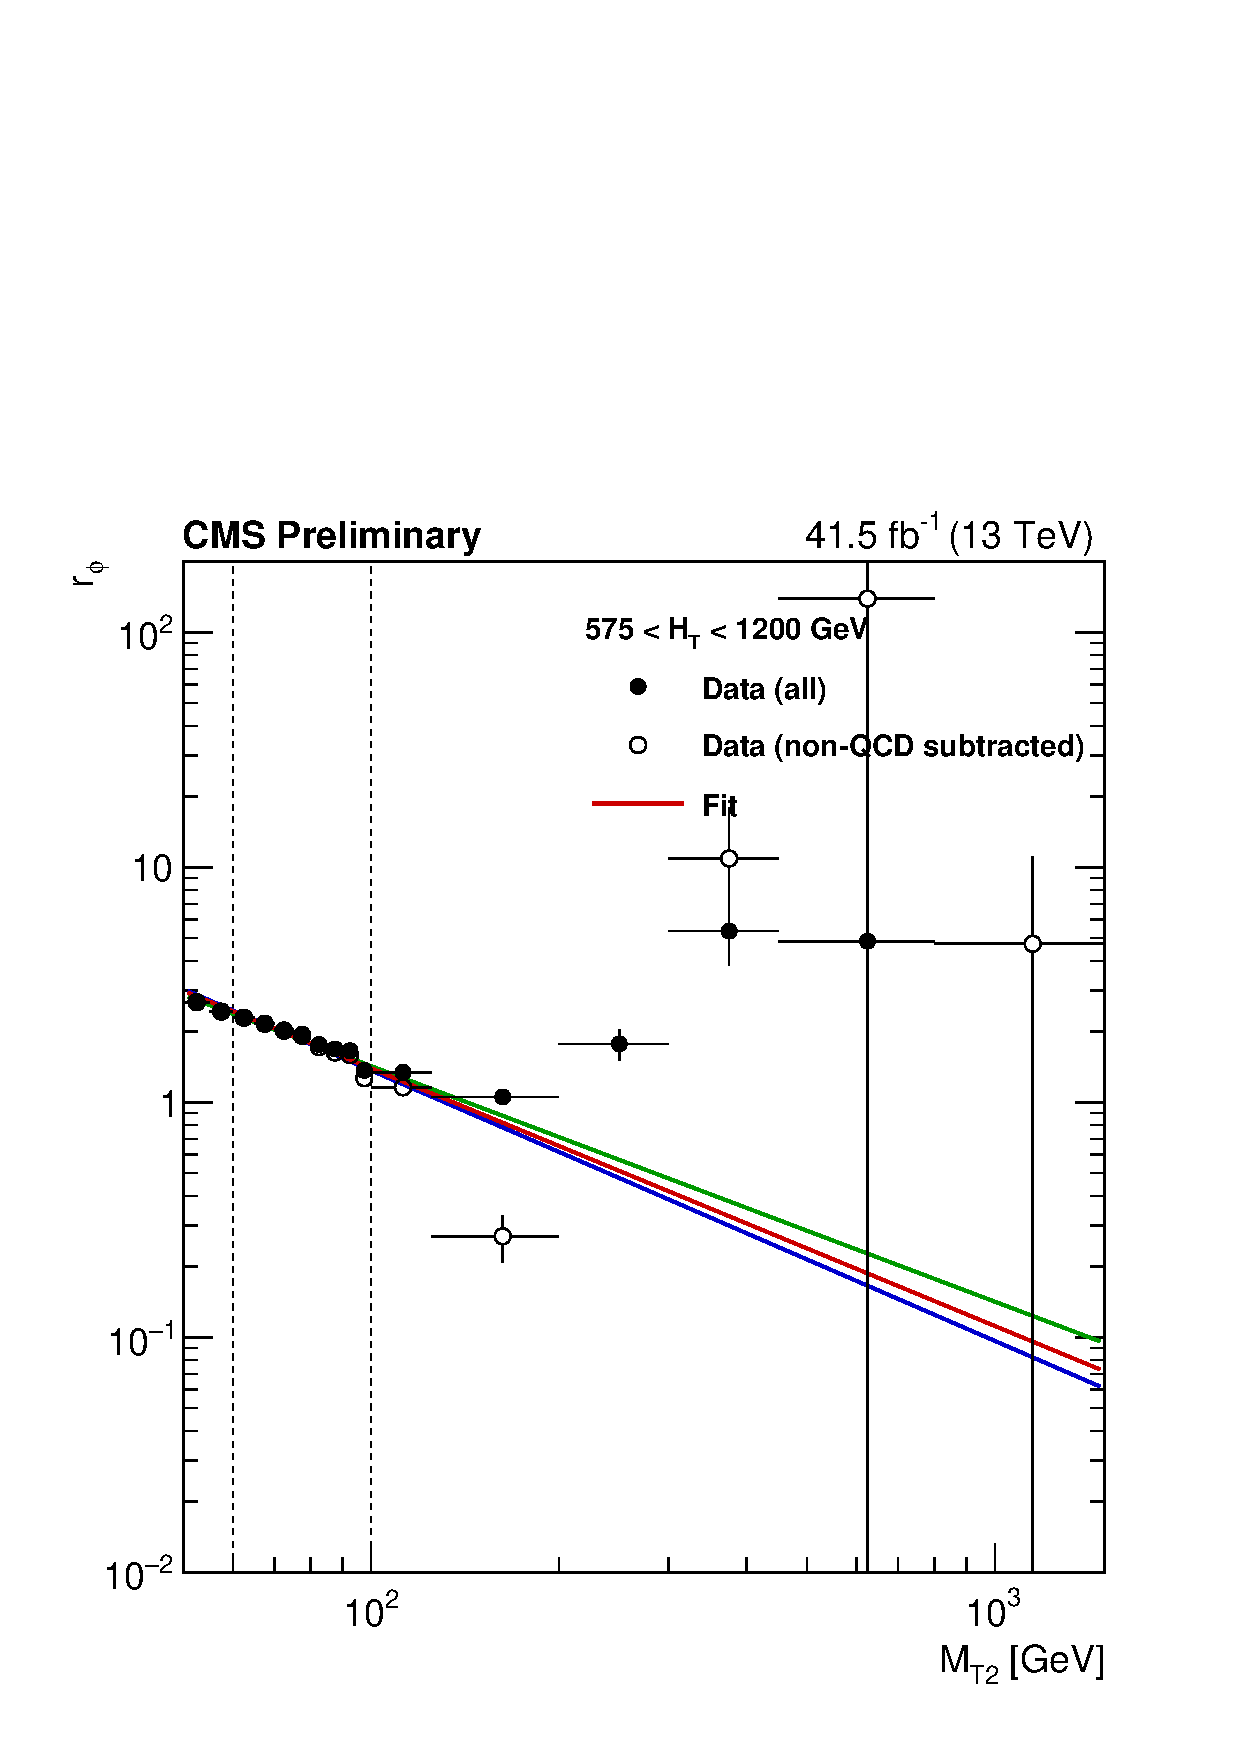
\includegraphics[width=0.48\linewidth]{figs/qcd/rphi_data_ht575to1200.pdf}
  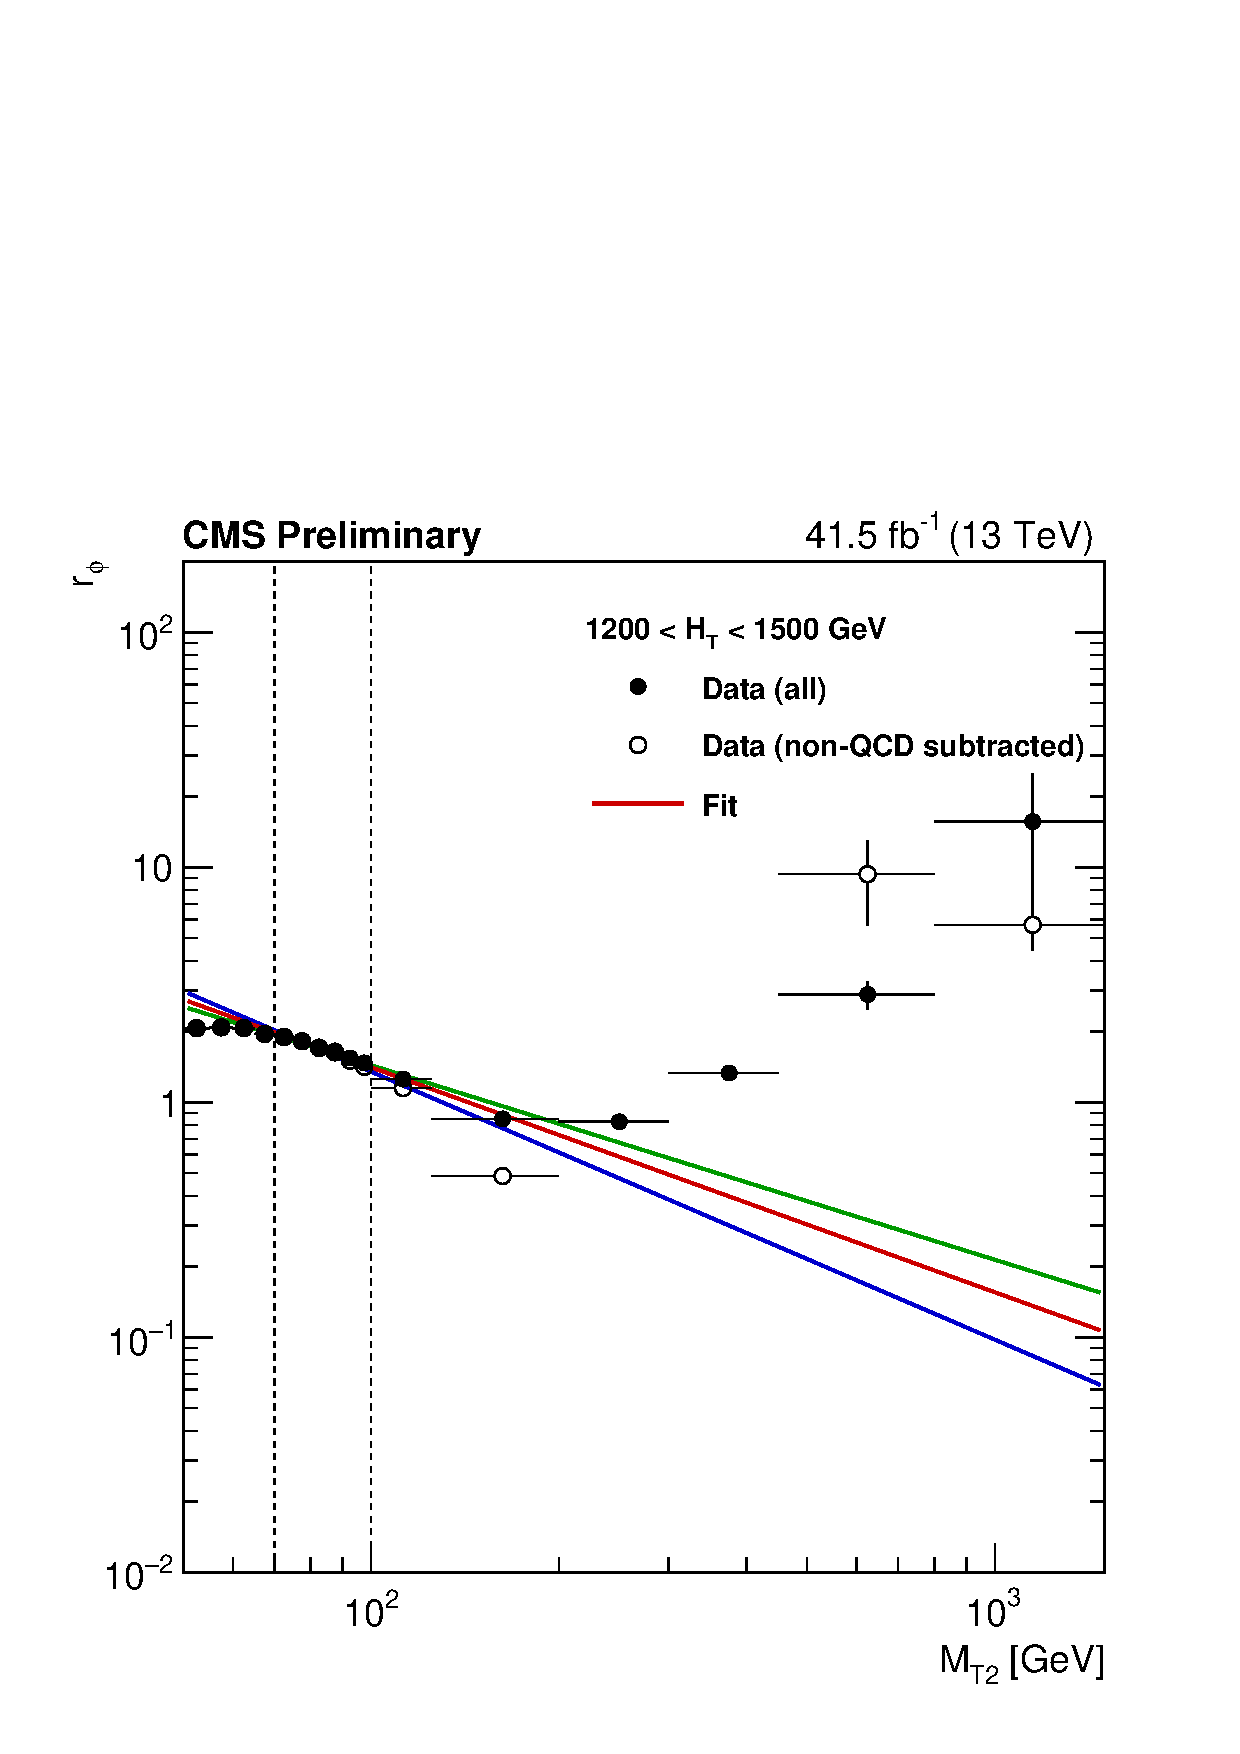
\includegraphics[width=0.48\linewidth]{figs/qcd/rphi_data_ht1200to1500.pdf}
  \caption{Example measurements of $r_\phi(\mttwo)$ in 2017 data, 
    for the medium and high \Ht regions. Black points are straight from data;
    white points have contribution from electroweak MC subtracted off from 
    both the numerator and denominator. Vertical dashed lines show the fit region.
    The red line is the central fit; the green and blue lines show the variations
    from extending the fit window one bin on the low or high edge, respectively.}
  \label{fig:rphi}
\end{figure}

\begin{figure}
  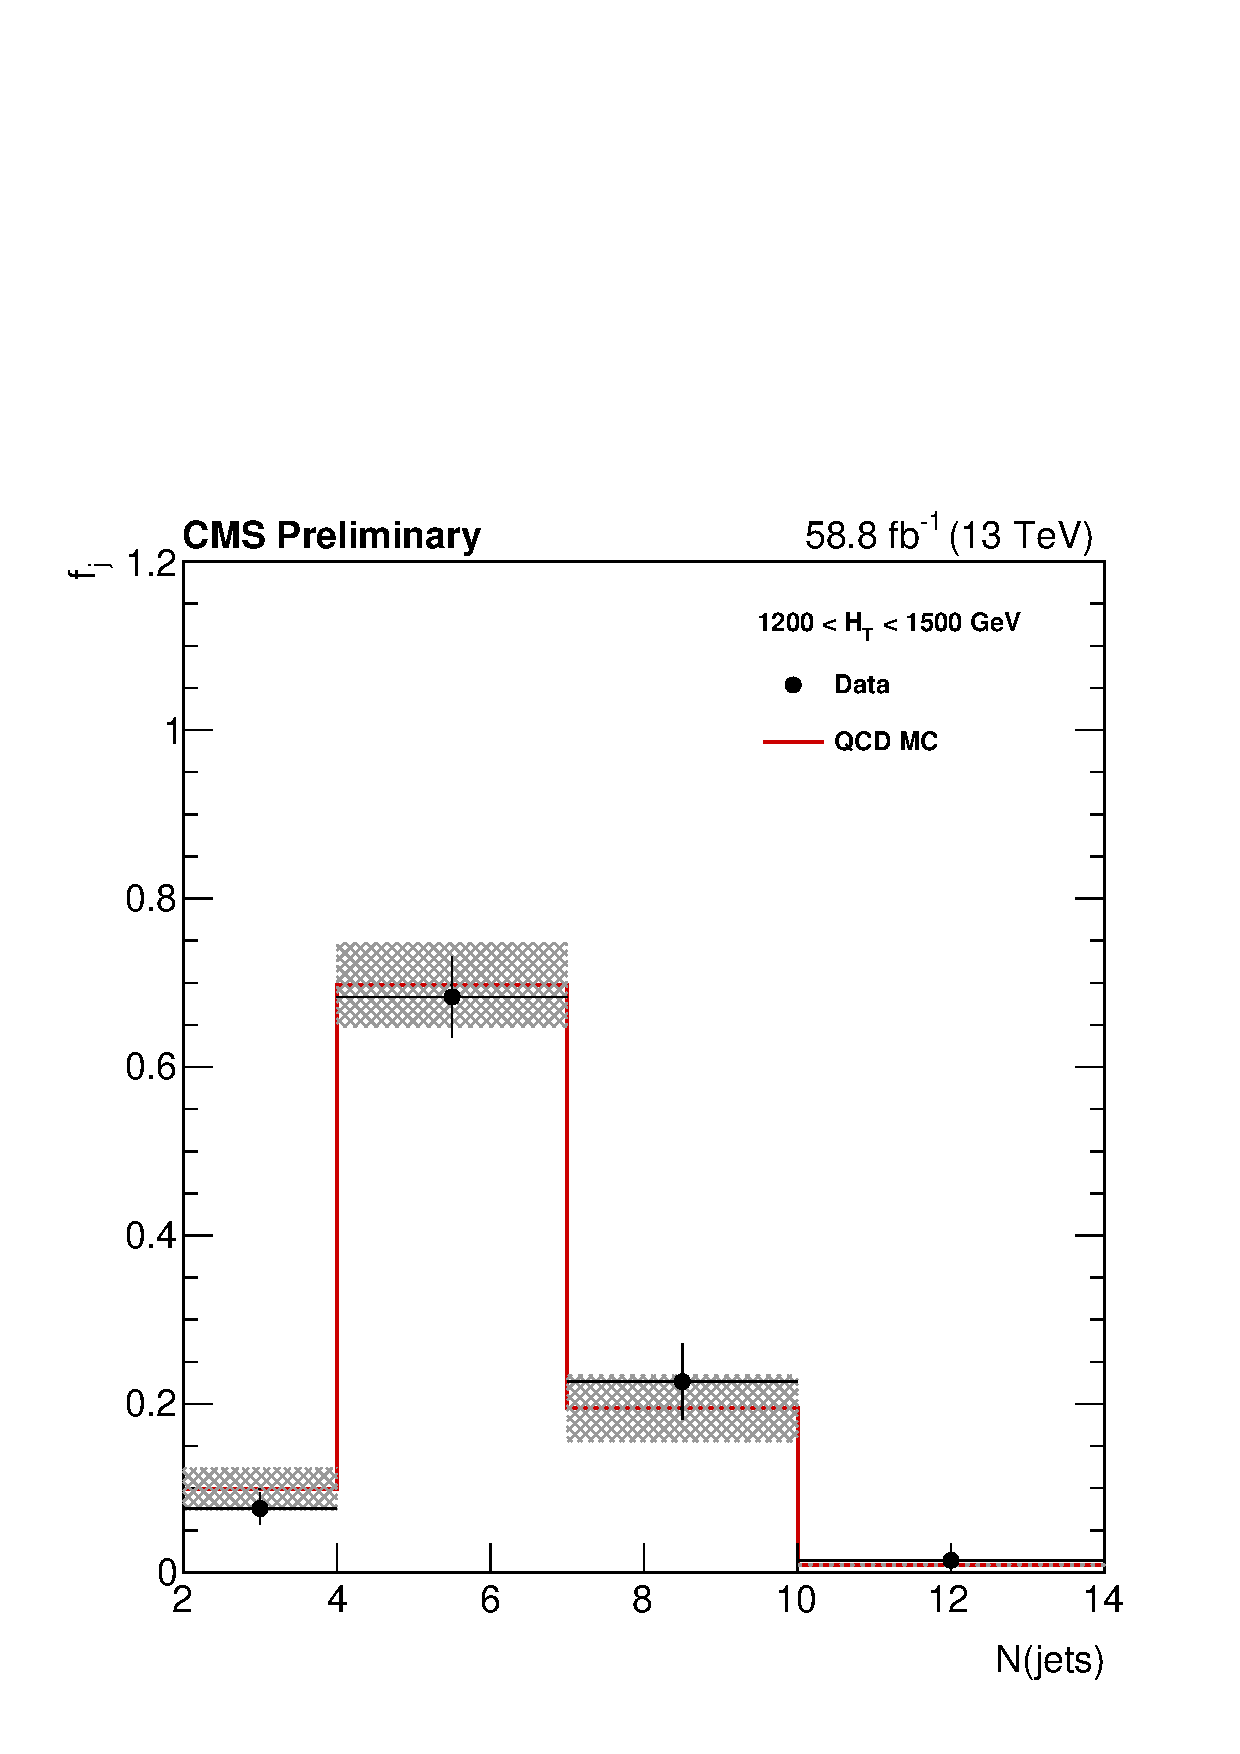
\includegraphics[width=0.48\linewidth]{figs/qcd/fj_ht1200to1500.pdf}
  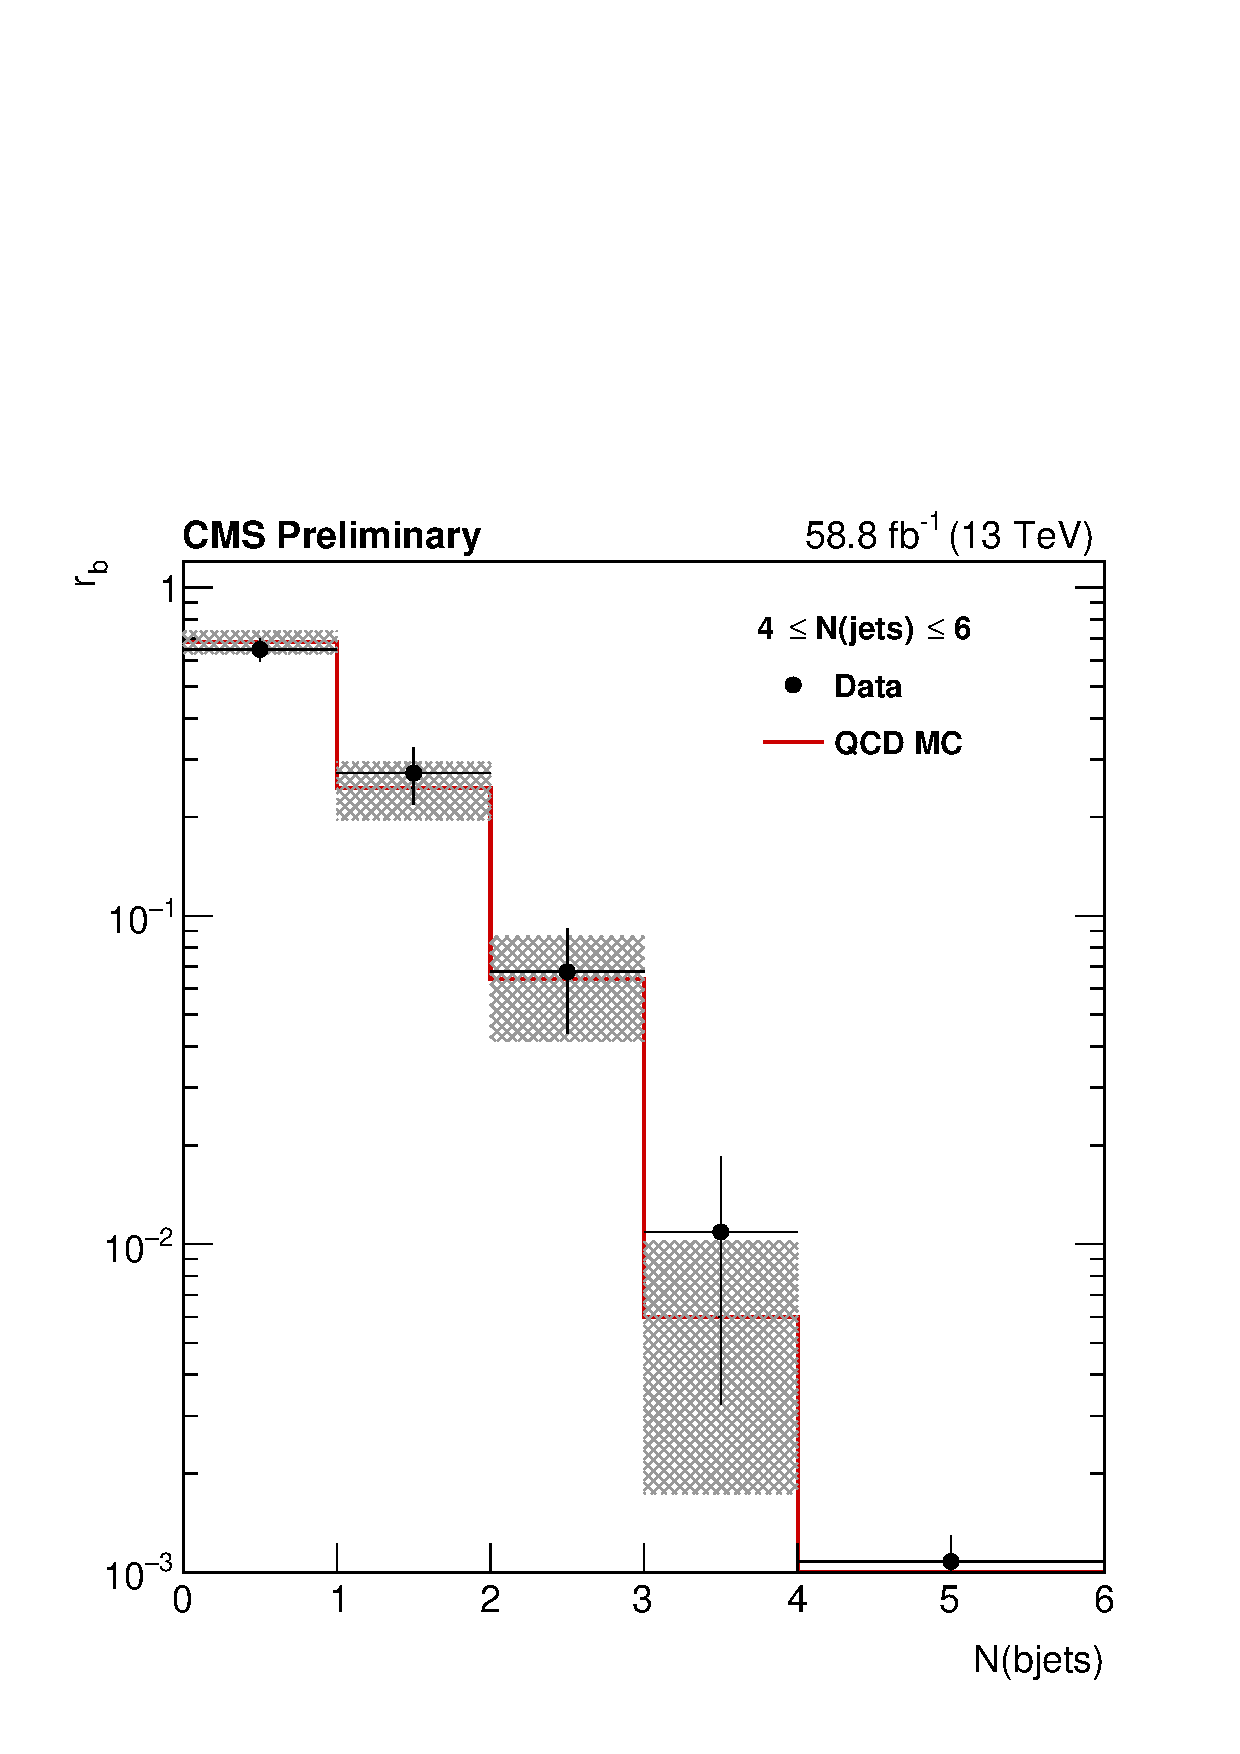
\includegraphics[width=0.48\linewidth]{figs/qcd/rb_j4to6.pdf}
  \caption{Transfer factors $f_j$ (left) and $r_b$ (right) measured in 2018 data. $f_j$
    is shown for $1200\leq\Ht<1500$\GeV, and $r_b$ is shown for $4\leq\njets\leq6$.
    Data agrees with simulation within the uncertainties.
}
  \label{fig:fjrb}
\end{figure}

Each event in the low-\dpmin control region (integrated across \njets and \nbtags)
 is weighted by $r_\phi(\mttwo)$ to get its contribution to the signal region.
It remains to distribute events among the \njets and \nbtags bins. This is done through
transfer factors $f_j$ and $r_b$. The first, $f_j$ is the fraction of events falling into a particular
\njets bin, and the second, $r_b$, is the fraction of events in a given \njets bin falling into a particular
\nbtags bin. It is found through simulation that both $f_j$ and $r_b$ 
are invariant with respect to $\mttwo$, and $r_b$ is invariant with respect to \Ht.
It is further found that the shapes are equivalent at $\dpmin < 0.3$ and $\dpmin >0.3$.
These facts allow us to measure $f_j$ and $r_b$ in a QCD-enriched control region ($\dpmin<0.3$,
$100 < \mttwo < 200$\GeV), $f_j$ in bins of \Ht and $r_b$ in bins of \njets.
Example measurements of $f_j$ and $r_b$ in 2018 data are shown in Fig.~\ref{fig:fjrb}.

Once all three of $r_\phi$, $f_j$, and $r_b$ are measured, we can get a final
signal region estimate as
\be
N_\mrm{SR}(\Ht,\njets,\nbtags,\mttwo) = \left(\sum_{\dpmin<0.3} r_\phi(\mttwo) \right) \cdot f_j(\Ht) \cdot r_b(\njets),
\ee
where the sum is taken over all events in a given \Ht region, inclusively in \njets and \nbtags.

\section{Overview of Rebalance and Smear}

While the $\Delta\phi$-ratio method has been used as the primary multijet estimation technique
in the past, there are a number of motivations to look for a better, more robust method.
Most importantly, the $\Delta\phi$-ratio method relies on a fairly severe extrapolation 
($r_\phi$ is measured in $60 < \mttwo < 100$\GeV, and is used to predict signal region 
yields at $\mttwo>200$\GeV), with no way to explicitly check its validity in the 
region of interest. Moreover, the power law fit function itself is empirically derived
from simulation, with no underlying theoretical motivation that would give one confidence
in its applicability.

An alternate method that is used as the primary multijet estimation technique in this 
iteration of the analysis is known as Rebalance and Smear (\rs).
The method consists of two distinct steps. The first, ``rebalancing'', seeks to adjust
the \pt of jets in multijet events such that the resulting \ptmiss is approximately zero,
with the aim of reproducing the true hard-scatter event which has no \ptmiss.
This is performed through a likelihood maximization, accounting for jet energy resolution.
The output of the rebalancing is an inclusive sample of multijet events with approximately
zero \ptmiss that are used as a seed for the second step, the ``smearing''. In this step, the
\pt values of the rebalanced jets are smeared according to jet response functions, in order
to model the instrumental effects that lead to nonzero \ptmiss. The smearing step is repeated many
times for each rebalanced event, which allows the accumulation of events in the tails
of kinematic distributions such as \ptmiss and \mttwo and for a more precise estimate 
of the multijet background in the signal regions.

Both the rebalancing and smearing steps make use of ``jet response templates'', which are distributions
of the ratio of reconstructed jet \pt to generator-level jet \pt. The templates are derived from simulation
in bins of jet \pt and $\eta$, separately for b-tagged and non-b-tagged jets. Details on the derivation
of the templates are given in Sec.~\ref{sec:jrt}.

For \rs in data, events from pure-\Ht triggers are used. Events with $\Ht<1200\GeV$ come
from prescaled triggers, and get weighted by the corresponding event-level prescale value in the final
prediction.

In addition to the trigger selections, events must contain at least one good vertex, two jets
with $\pt>10\GeV$, and pass the standard event cleaning filters in order to be used in the \rs.
No other selections are applied.

\subsection{Rebalancing}
The rebalancing procedure adjusts the \pt of jets in an event with the aim of reproducing the true
hard-scatter event which has no \ptmiss. Note that only the magnitude of the jet \pt is modified,
while the jet direction remains unchanged.

Of all jets in the event, a jet qualifies for use in the rebalancing and smearing procedure if it has $\pt>10$\GeV,
and if it is not identified as a jet from pileup in the case that $\pt<100$\GeV.
All other jets are left unchanged but are still used in the calculation of \vMet and other jet-related quantities.
An event with $n$ qualifying jets is rebalanced by varying the $p_\text{T}^\text{reb}$ of each jet to maximize the likelihood function
\be
\label{eq:rebalance_likelihood}
L = \prod_{i=1}^n \text{P} ( \ptireco | \ptireb ) 
   \times G\left( \frac{p_{\text{T},\text{reb,x}}^\text{miss}}{\sigma_\text{T}^{\text{soft}}}\right) 
   \times G\left( \frac{p_{\text{T},\text{reb,y}}^\text{miss}}{\sigma_\text{T}^{\text{soft}}}\right),
\ee
where
\be
\label{eq:G_def}
G(x) \equiv e^{-x^2/2}
\end{equation}
and
\begin{equation}
\label{eq:reb_met_def}
\vSS{p}{\mrm{T,reb}}{\mrm{miss}} \equiv \vSS{p}{\mrm{T}}{\mrm{miss}} - \sum_{i=1}^n \left( \vSS{p}{\mrm{T},i}{\mrm{reb}} - \vSS{p}{\mrm{T},i}{\mrm{reco}} \right).
\end{equation}

The term $\text{P} ( \ptireco | \ptireb )$ in Eq.~\ref{eq:rebalance_likelihood} is the probability for a jet with $\pt$ of
\ptireb to be assigned a $\pt$ of \ptireco after reconstruction.
This probability is taken directly from the jet response templates.
The two $G(x)$ terms in Eq.~\ref{eq:rebalance_likelihood} enforce an approximate balancing condition.
The $\vSS{p}{\mrm{T,reb}}{\mrm{miss}}$ terms in Eq.~\ref{eq:rebalance_likelihood} represent the missing transverse momentum after rebalancing, and are obtained
by simply propagating to \vMet the changes in jet \pt from rebalancing.
For the balancing of the $x$ and $y$ components of the missing transverse momentum,
we use $\sigma_\text{T}^{\text{soft}}=20$\GeV, which is
approximately the width of the distributions of the $x$ and $y$ components of \vMet
in minimum bias events. This parameter represents the inherent missing energy due to low-\pt jets, unclustered energy, and jets from pileup that cannot be eliminated by rebalancing.
A systematic uncertainty is assessed to cover for the effects of the variation of $\sigma_\text{T}^\text{soft}$.

In practice, the likelihood maximization is done by minimizing $-\log L$ using \textsc{minuit} \cite{minuit} via \textsc{root}.
The minimization is done by finding the $n$ parameters $c_1,\dots,c_n$ such that
$\ptireb\equiv\frac{1}{c_i}\ptireco$ minimize $-\log L$. To calculate
$P(\ptireco|\ptireb)$ we look at the response template for jets with $\pt=\frac{1}{c_i}\ptireco$
and $\eta=\eta_i$ and find the probability of $c_i$. The rebalanced event will have jets with \pt
scaled by their corresponding $\frac{1}{c_i}$.

\subsection{Smearing}

Once a sample of rebalanced events has been obtained the next step is to smear the jets in these events many times. 
Each rebalanced event is smeared ($100 \times\mrm{prescale}$) times for data, or just 100 times for MC.
The number of smears is capped at 5000, and a corresponding extra weight is applied to events where $100 \times\mrm{prescale}>5000$.
For each smearing, the \pt of each jet in the rebalanced event is scaled by a random factor drawn from the corresponding jet response template. If an event
contains jets that were not considered in the rebalancing procedure (i.e. they have $\pt<10$\GeV, or have $\pt<100$\GeV and fail the pileup jet ID) 
then those jets remain in the event without any smearing. 

After the smearing has been done, all jet-related quantities (\Ht, \ptmiss, \mttwo, \dpmin, etc.) 
are recalculated and analysis selections are applied. Histograms are filled for each smeared event that passes the analysis
selections with a weight of $1/N_\mrm{smears}$. The \rs predictions for kinematic distributions and event yields are taken from these histograms.
For the purposes of calculating statistical uncertainty, multiple smears of the same input event are taken as fully correlated when filling histograms. For example, if an event
is smeared 100 times, and 3 of those smeared events populate a given histogram bin, then that bin is filled once with a weight of 3/100, rather than three separate
times with a weight of 1/100.

\section{Performance in Monte Carlo}

Figures \ref{Fig:rs_mc_ht_met_highht}--\ref{Fig:rs_mc_deltaphi_highht} show kinematic distributions from QCD Monte Carlo
and \rs based on the same QCD Monte Carlo after a loose selection of $\Ht > 1200$\GeV, $\ptmiss > 30$\GeV, and $\mttwo > 50$\GeV.
Figures \ref{Fig:rs_mc_ht_met_lowht}--\ref{Fig:rs_mc_deltaphi_lowht} show the same distributions but with $450 < \Ht < 1200$\GeV.
The \rs method models the shapes of these distributions quite well. There is an overall normalization difference of $\mathcal{O}$(few percent)
introduced by the \ptmiss and \mttwo cuts due to differences in modeling of very low \ptmiss events.

Figure \ref{Fig:rs_mc_comp_sr_ratio} shows Monte Carlo closure in the topological regions after the baseline selection.
Statistics are quite low in the straight MC, but yields agree reasonably well where comparison is possible.

\begin{figure}[htbp]
  \begin{center}
    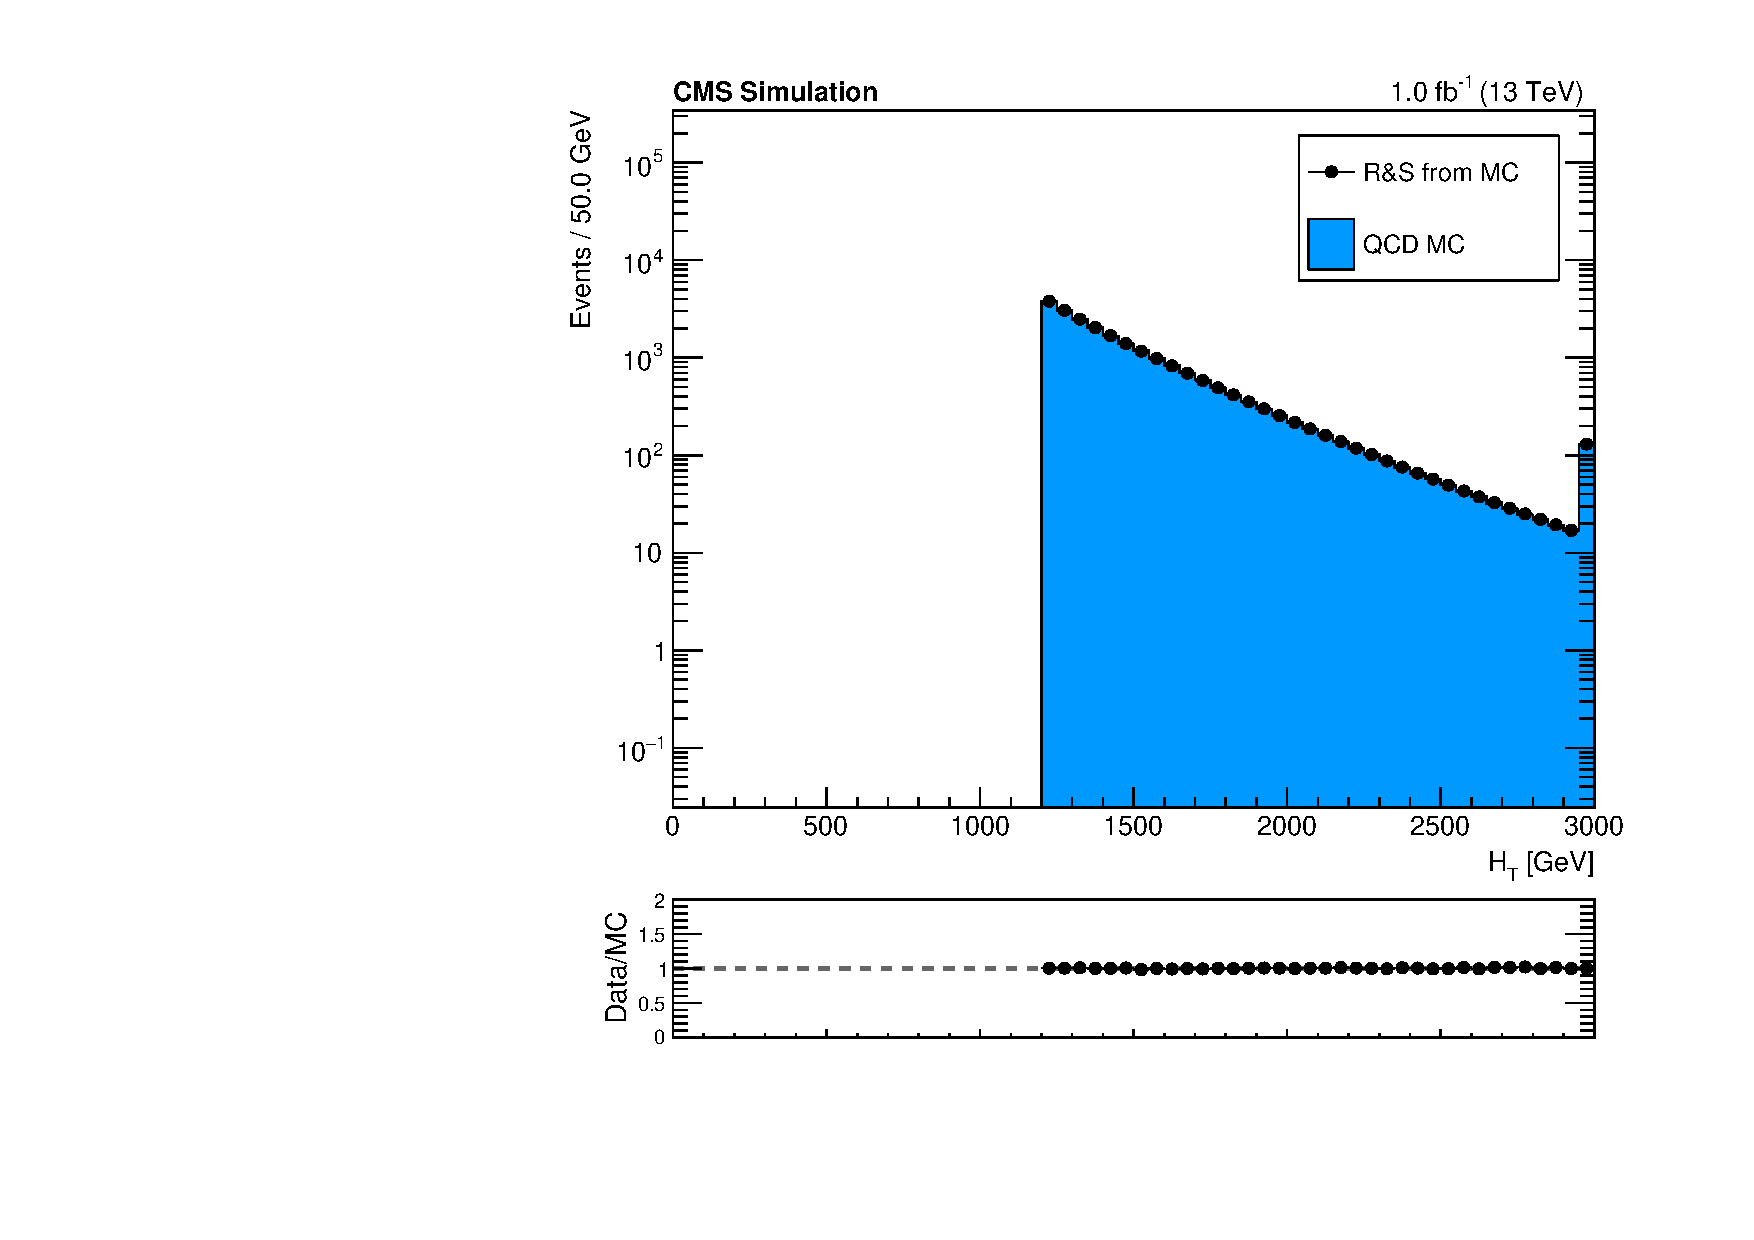
\includegraphics[width=0.46\textwidth]{figs/qcd/rs_mc/highht_ht.pdf}
    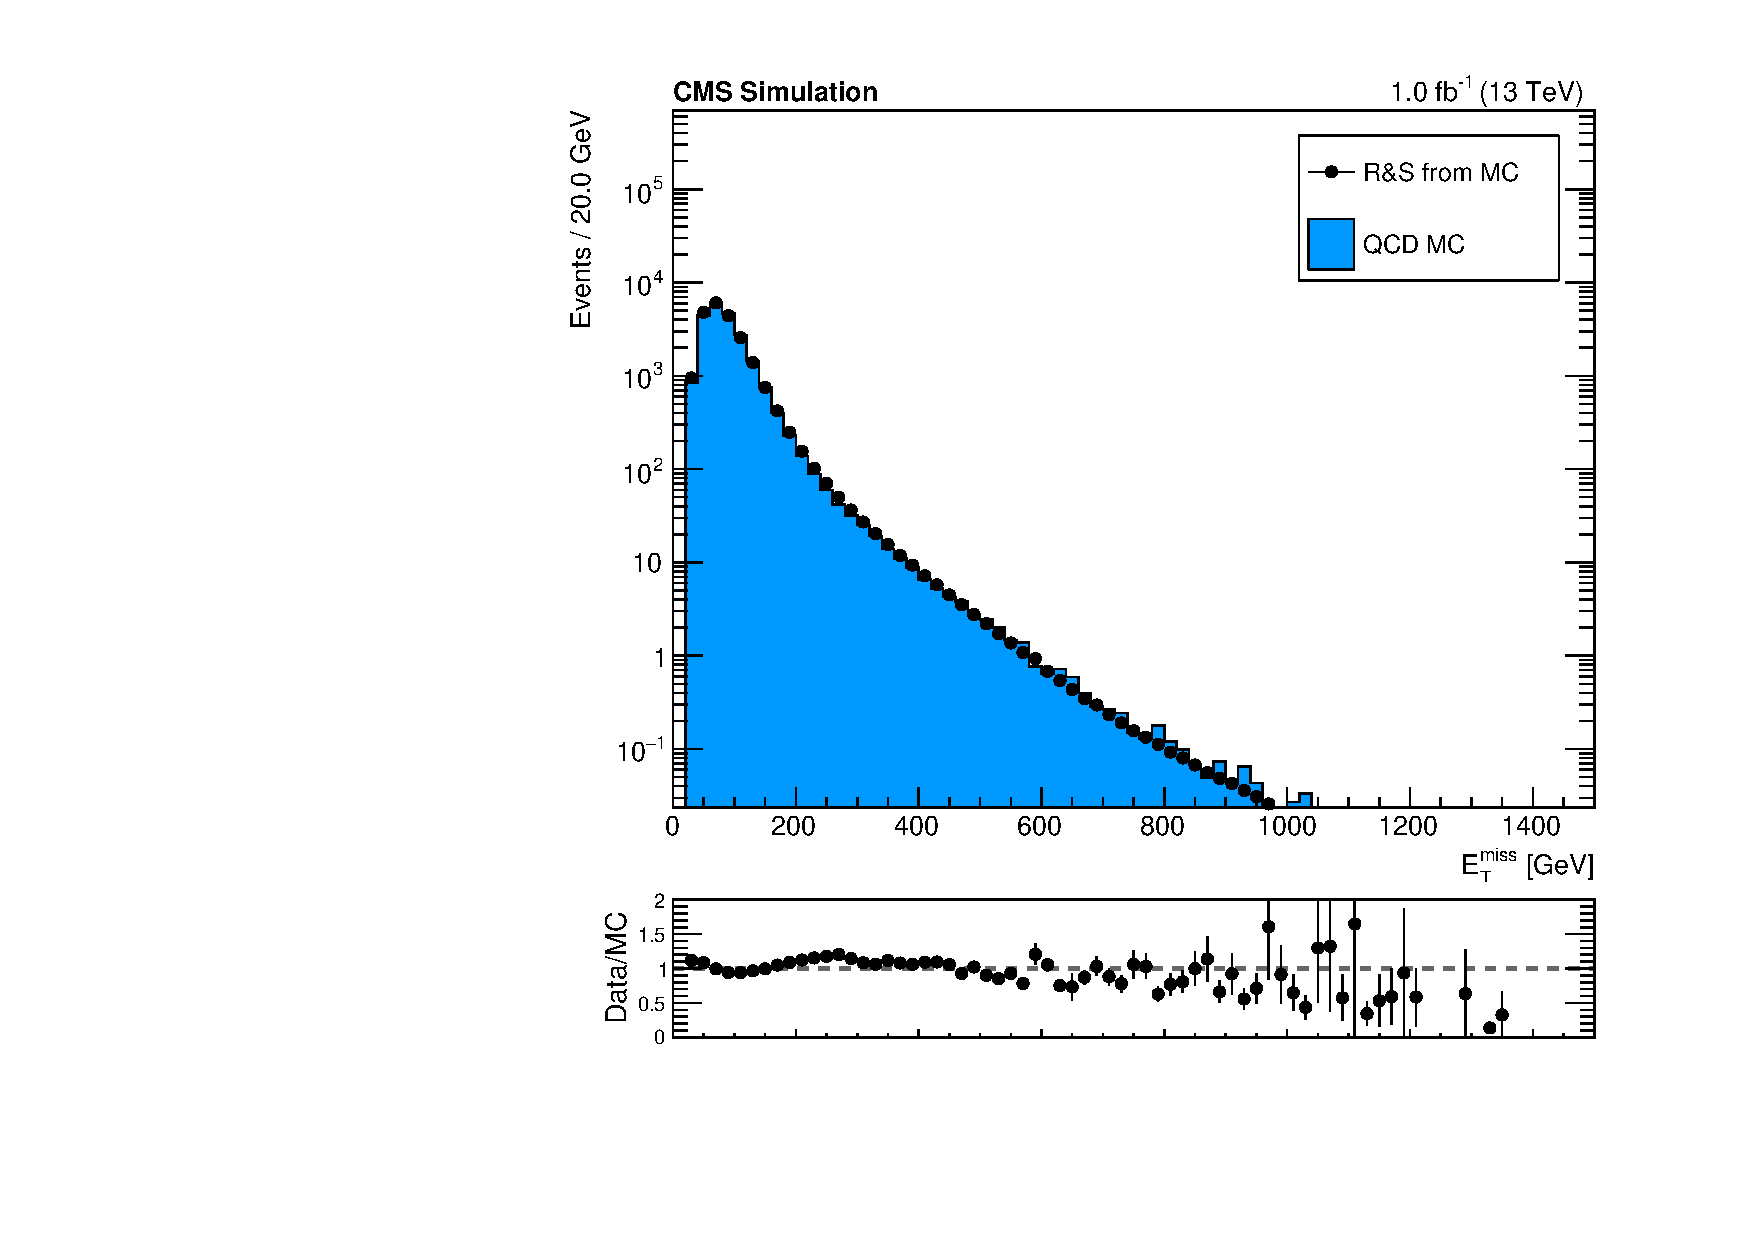
\includegraphics[width=0.46\textwidth]{figs/qcd/rs_mc/highht_met.pdf} \\
    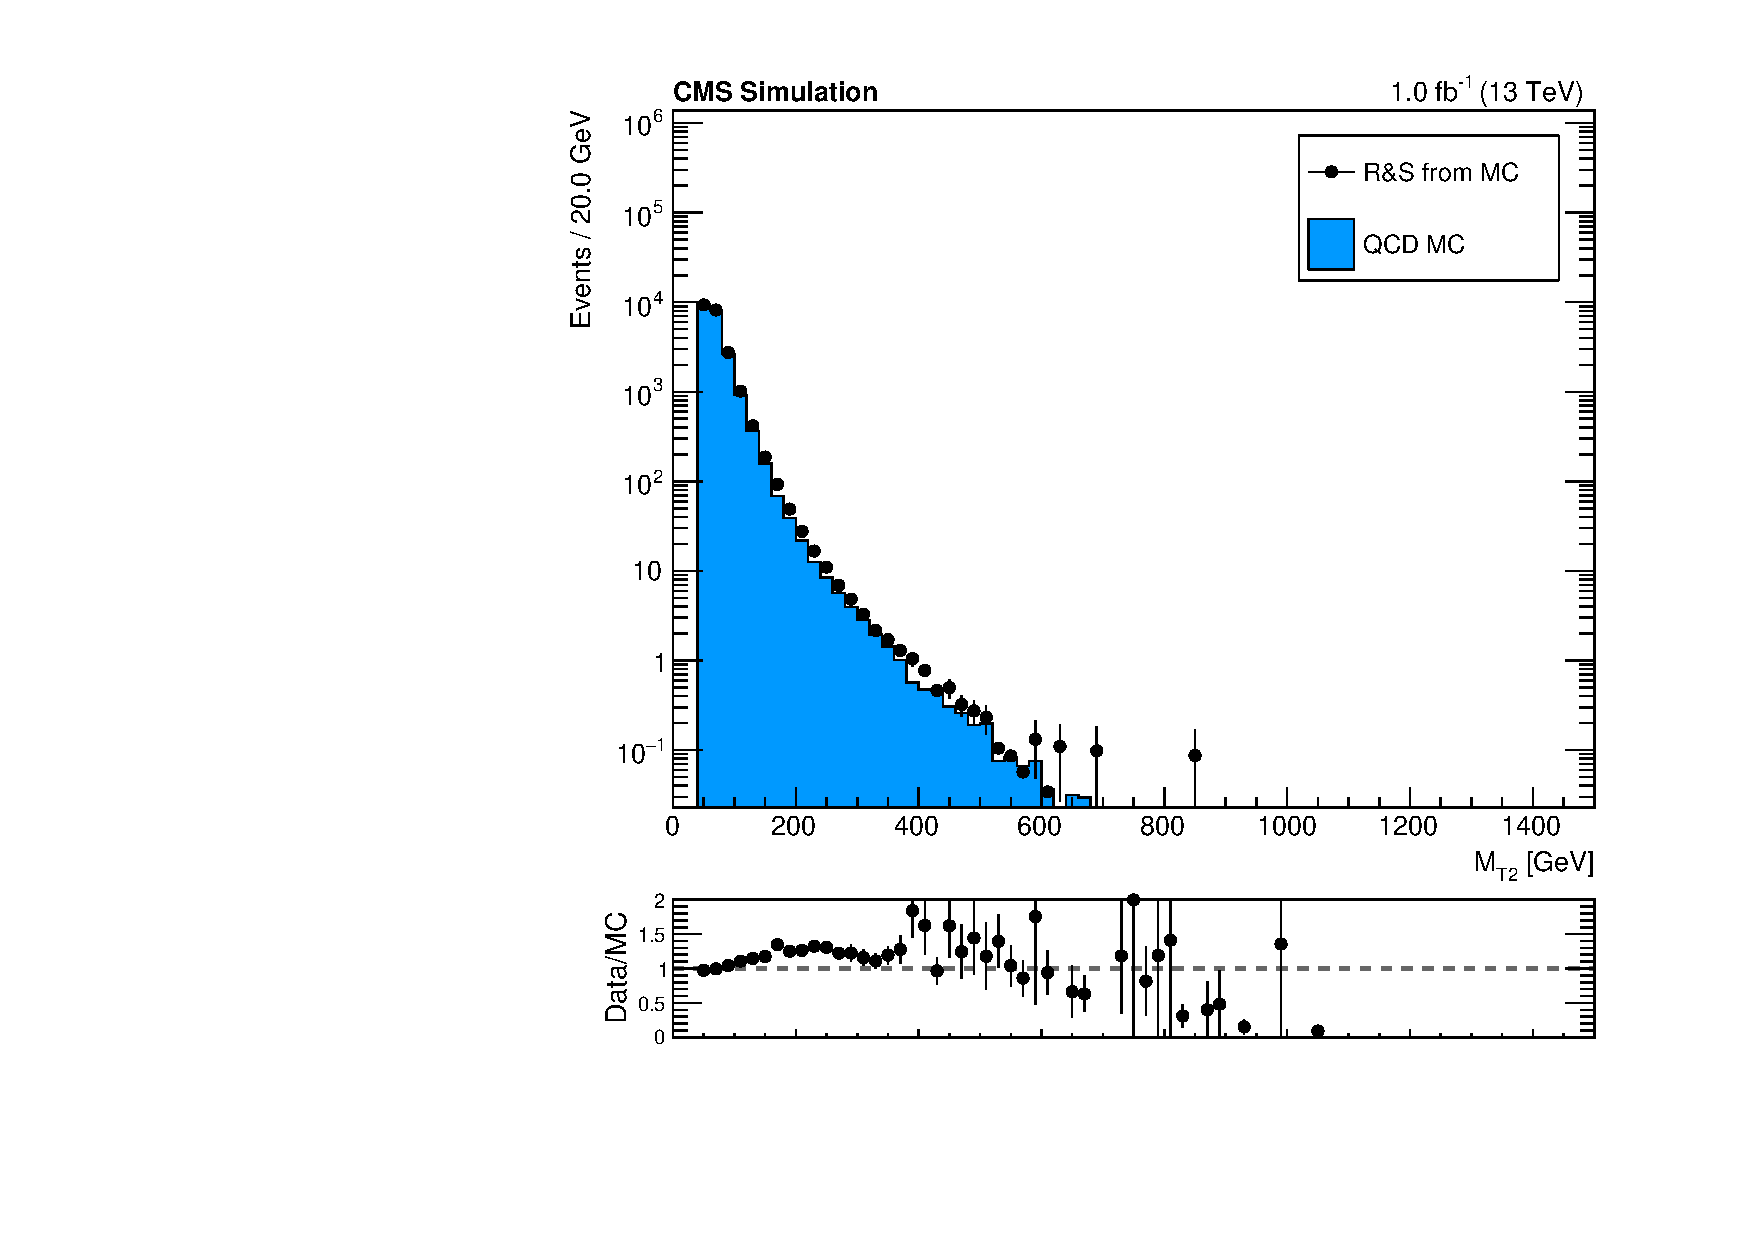
\includegraphics[width=0.46\textwidth]{figs/qcd/rs_mc/highht_mt2.pdf}
    \caption{\Ht, \ptmiss, and \mttwo distributions for Monte Carlo and \rs based on MC. The selection is $\Ht > 1200$\GeV, $\ptmiss > 30$\GeV and $\mttwo > 50$\GeV.
            }
    \label{Fig:rs_mc_ht_met_highht}
  \end{center}
\end{figure}

\begin{figure}[htbp]
  \begin{center}
    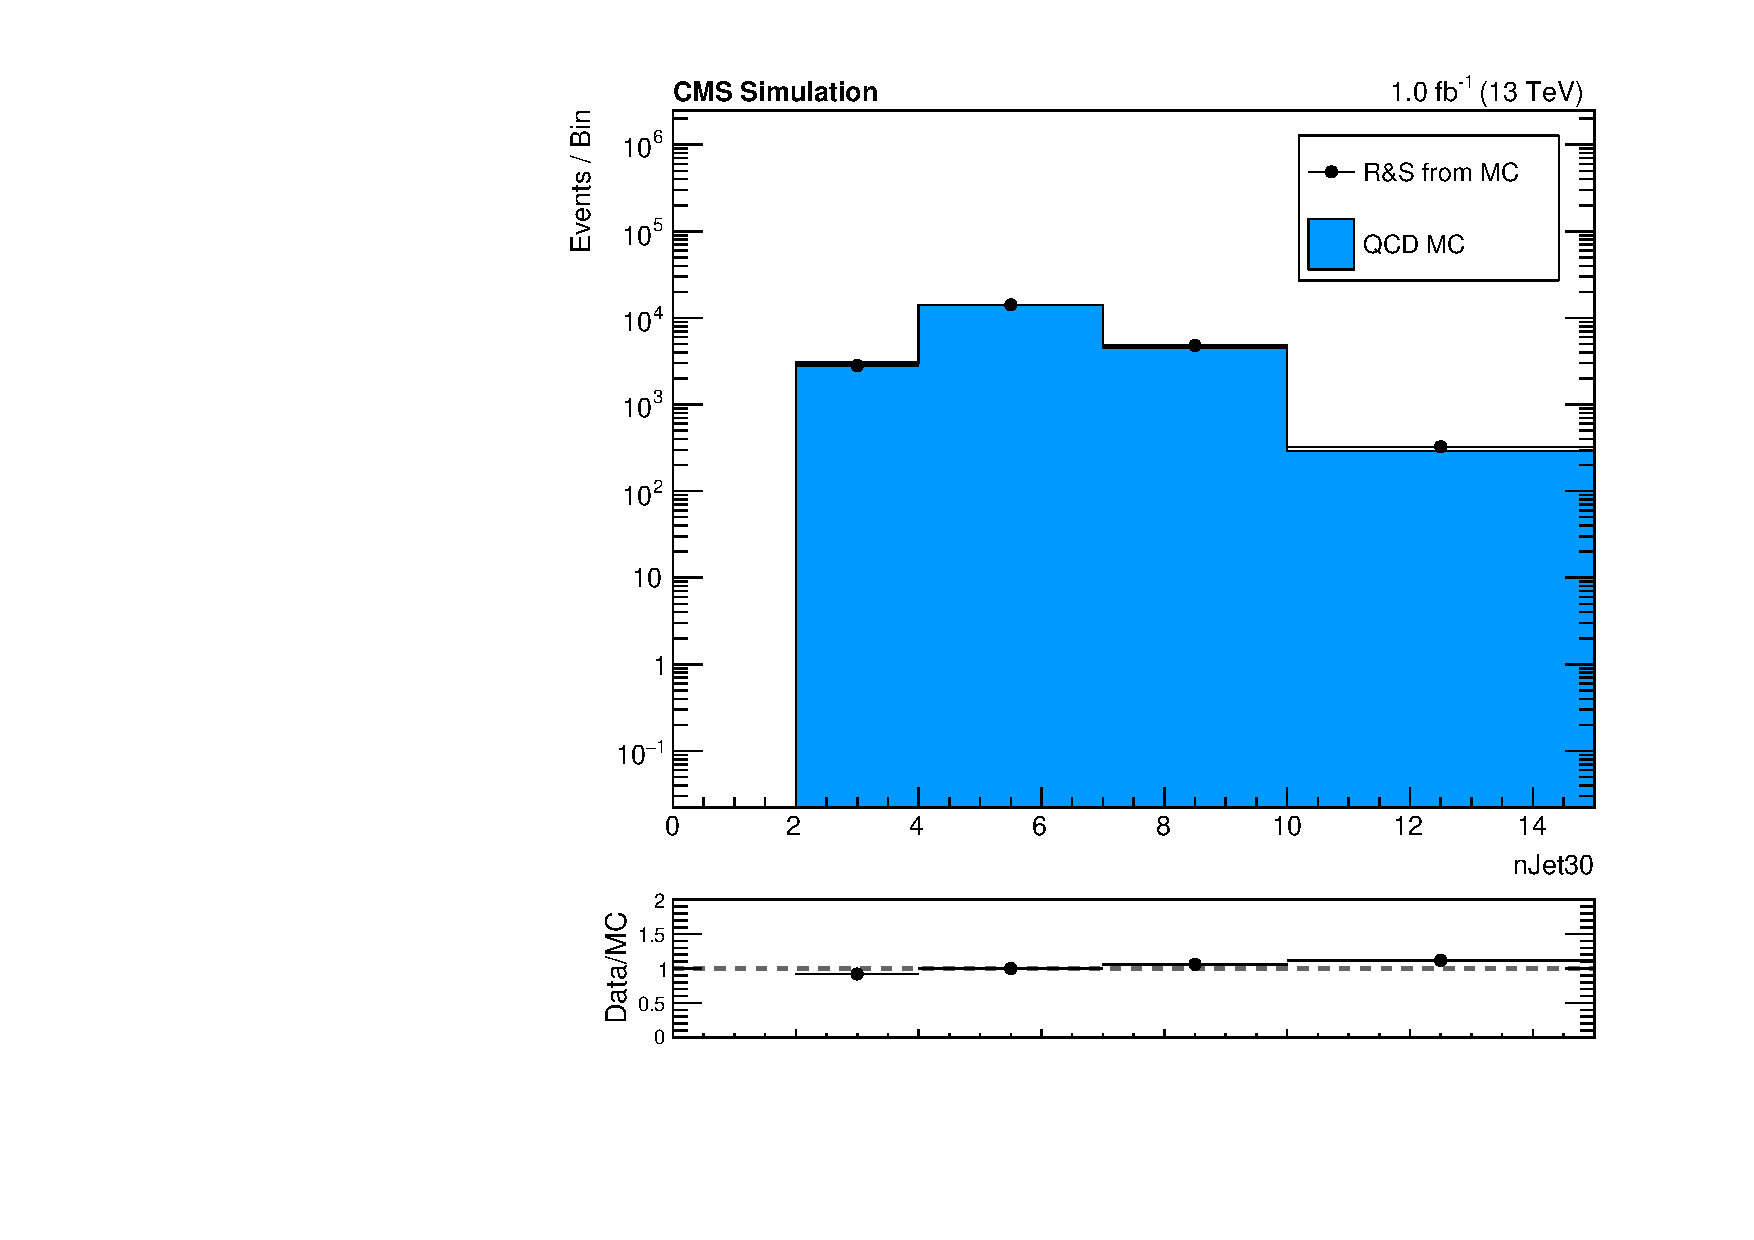
\includegraphics[width=0.46\textwidth]{figs/qcd/rs_mc/highht_nJet30.pdf}
    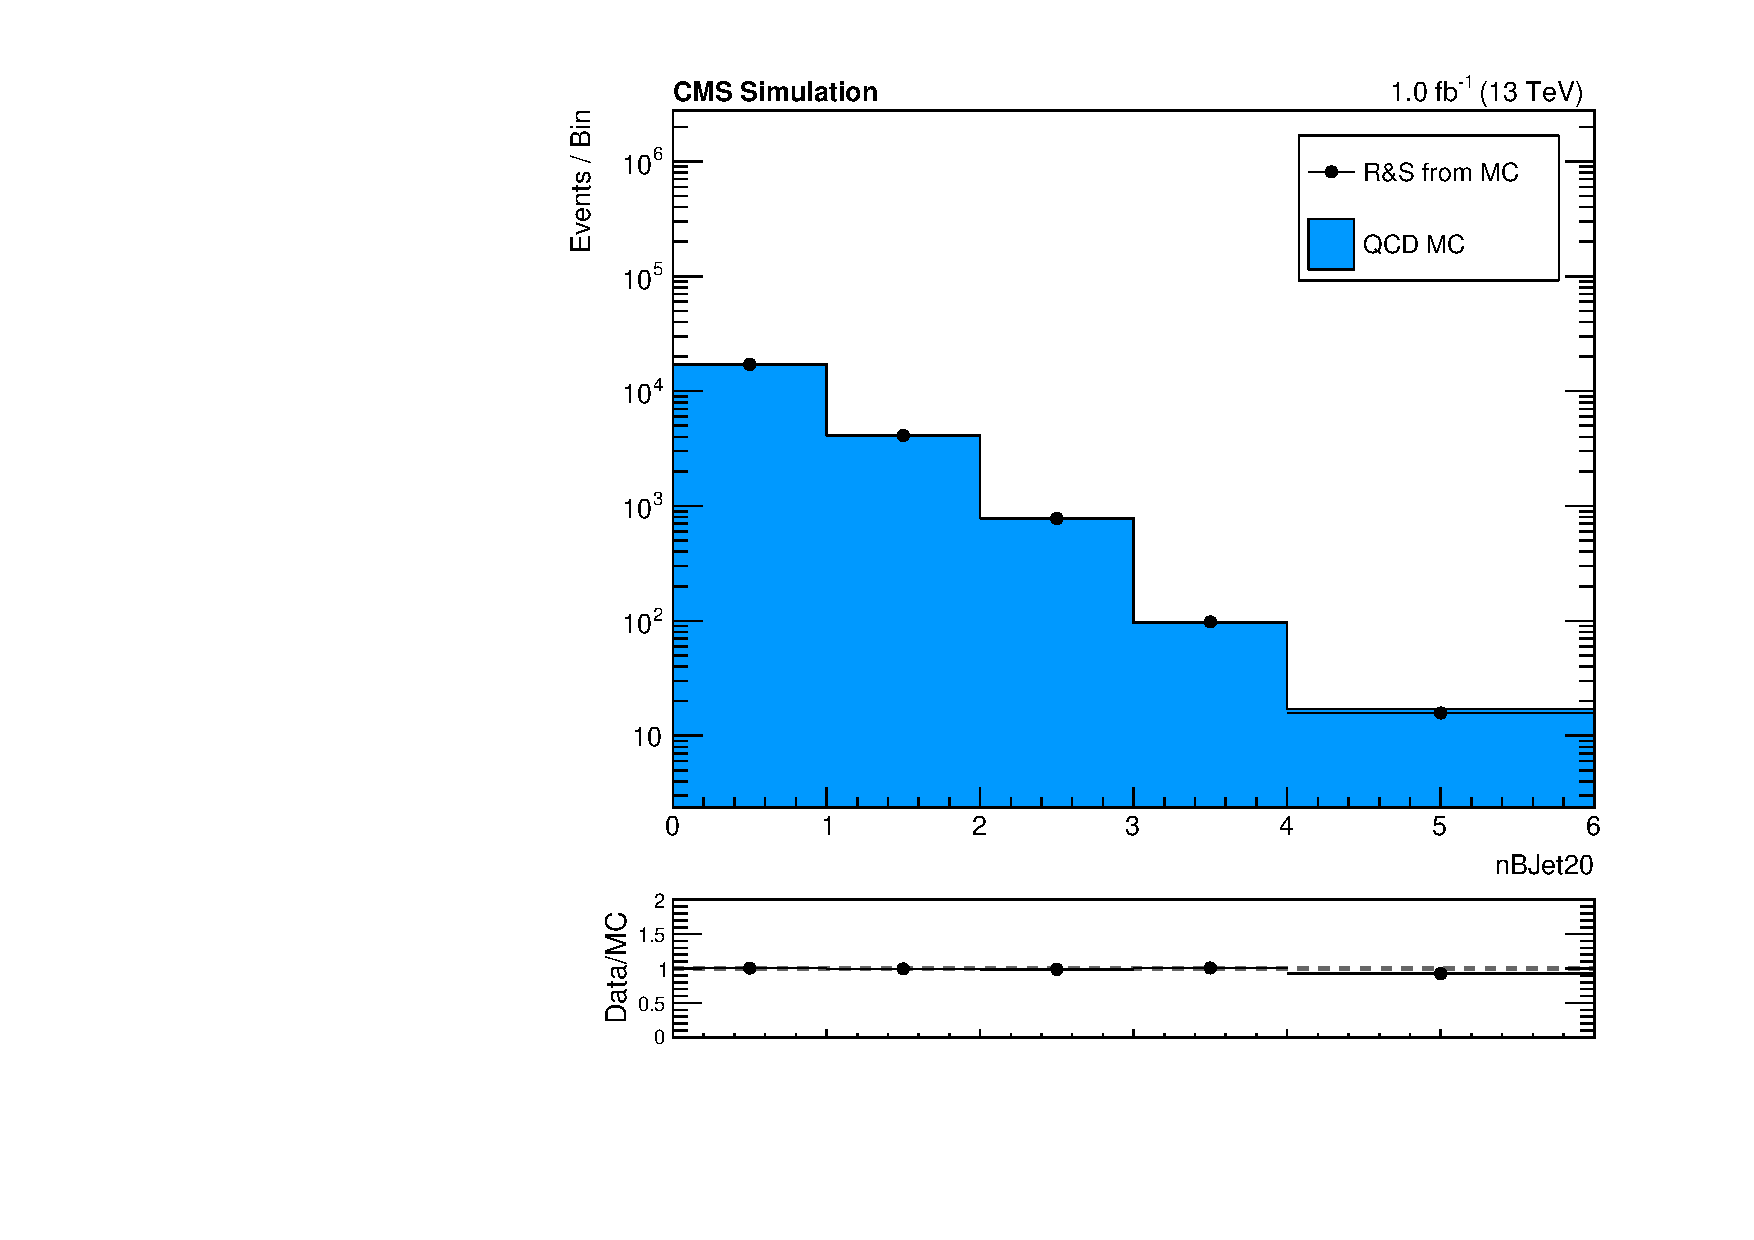
\includegraphics[width=0.46\textwidth]{figs/qcd/rs_mc/highht_nBJet20.pdf} \\
    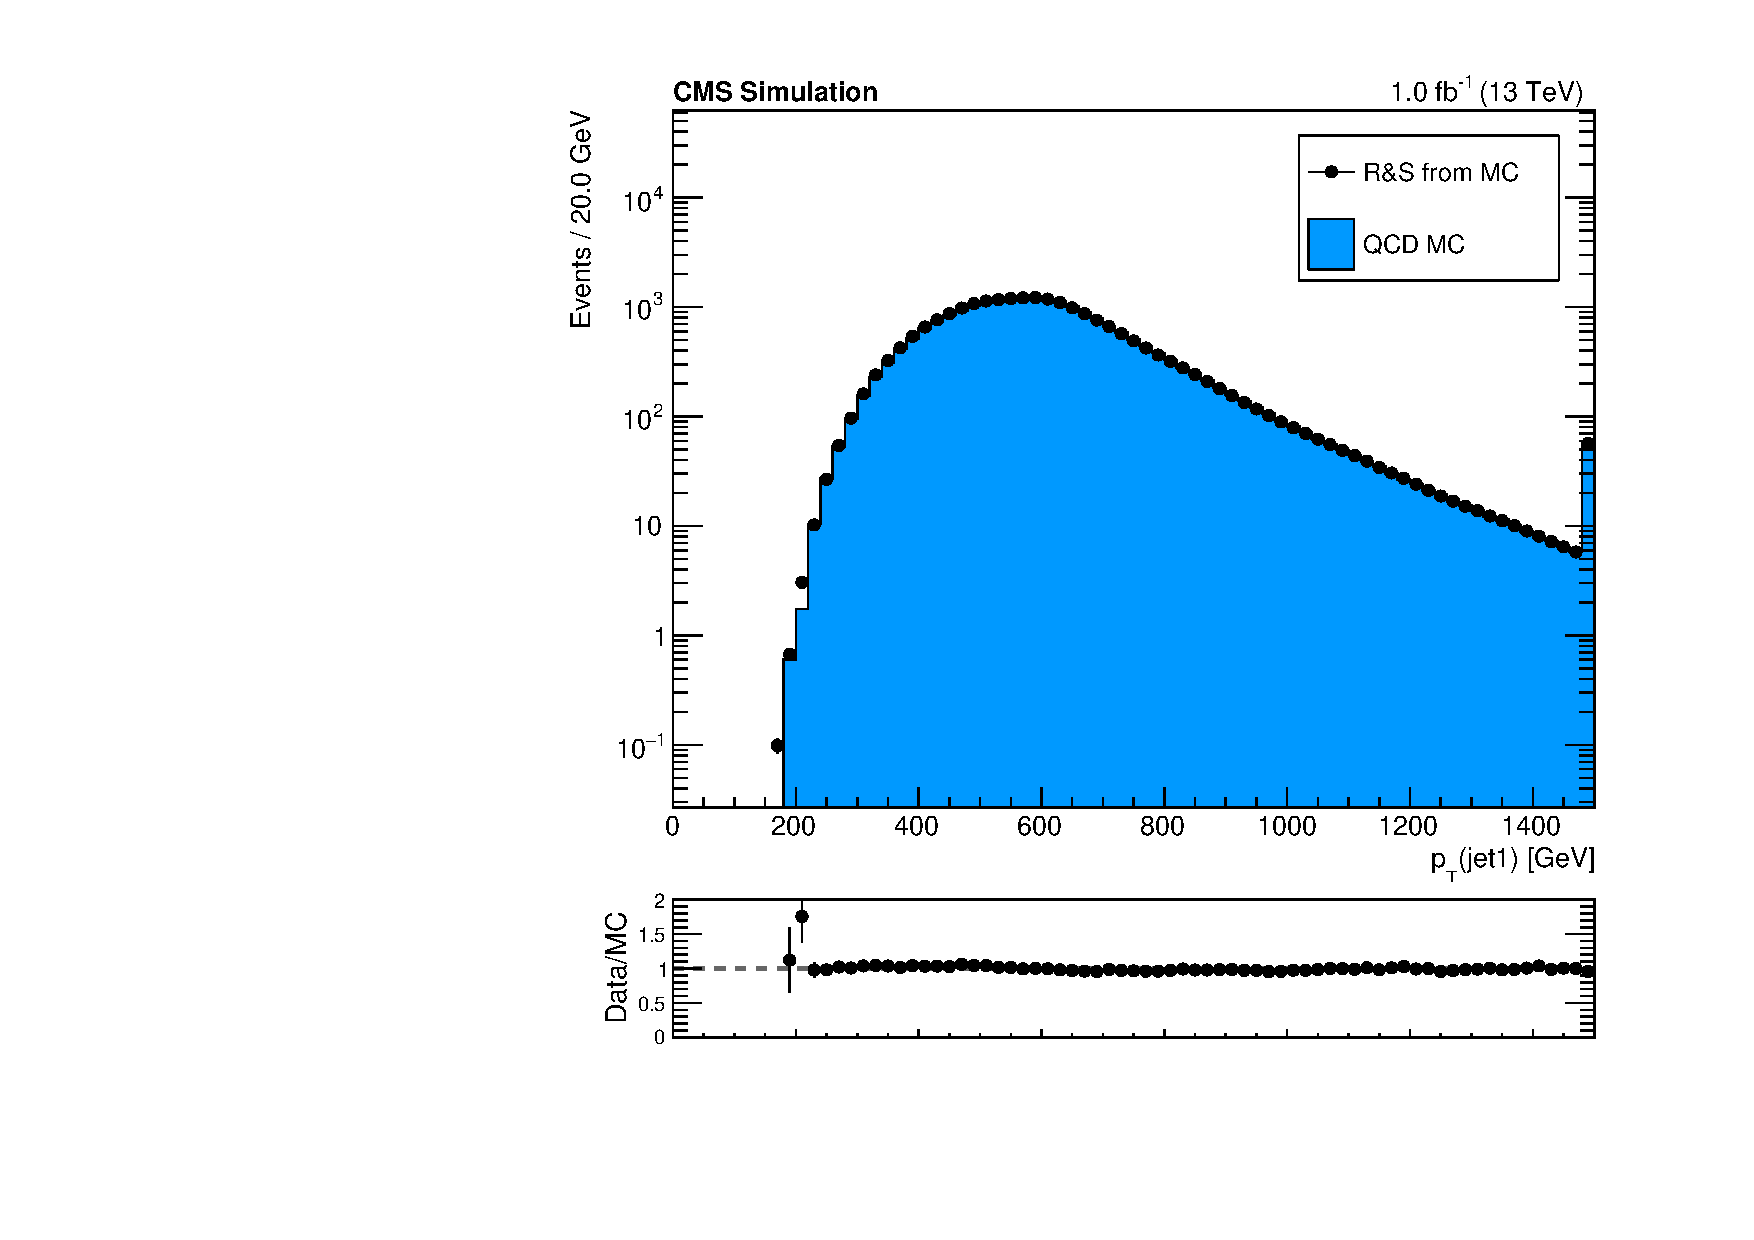
\includegraphics[width=0.46\textwidth]{figs/qcd/rs_mc/highht_J0pt.pdf}
    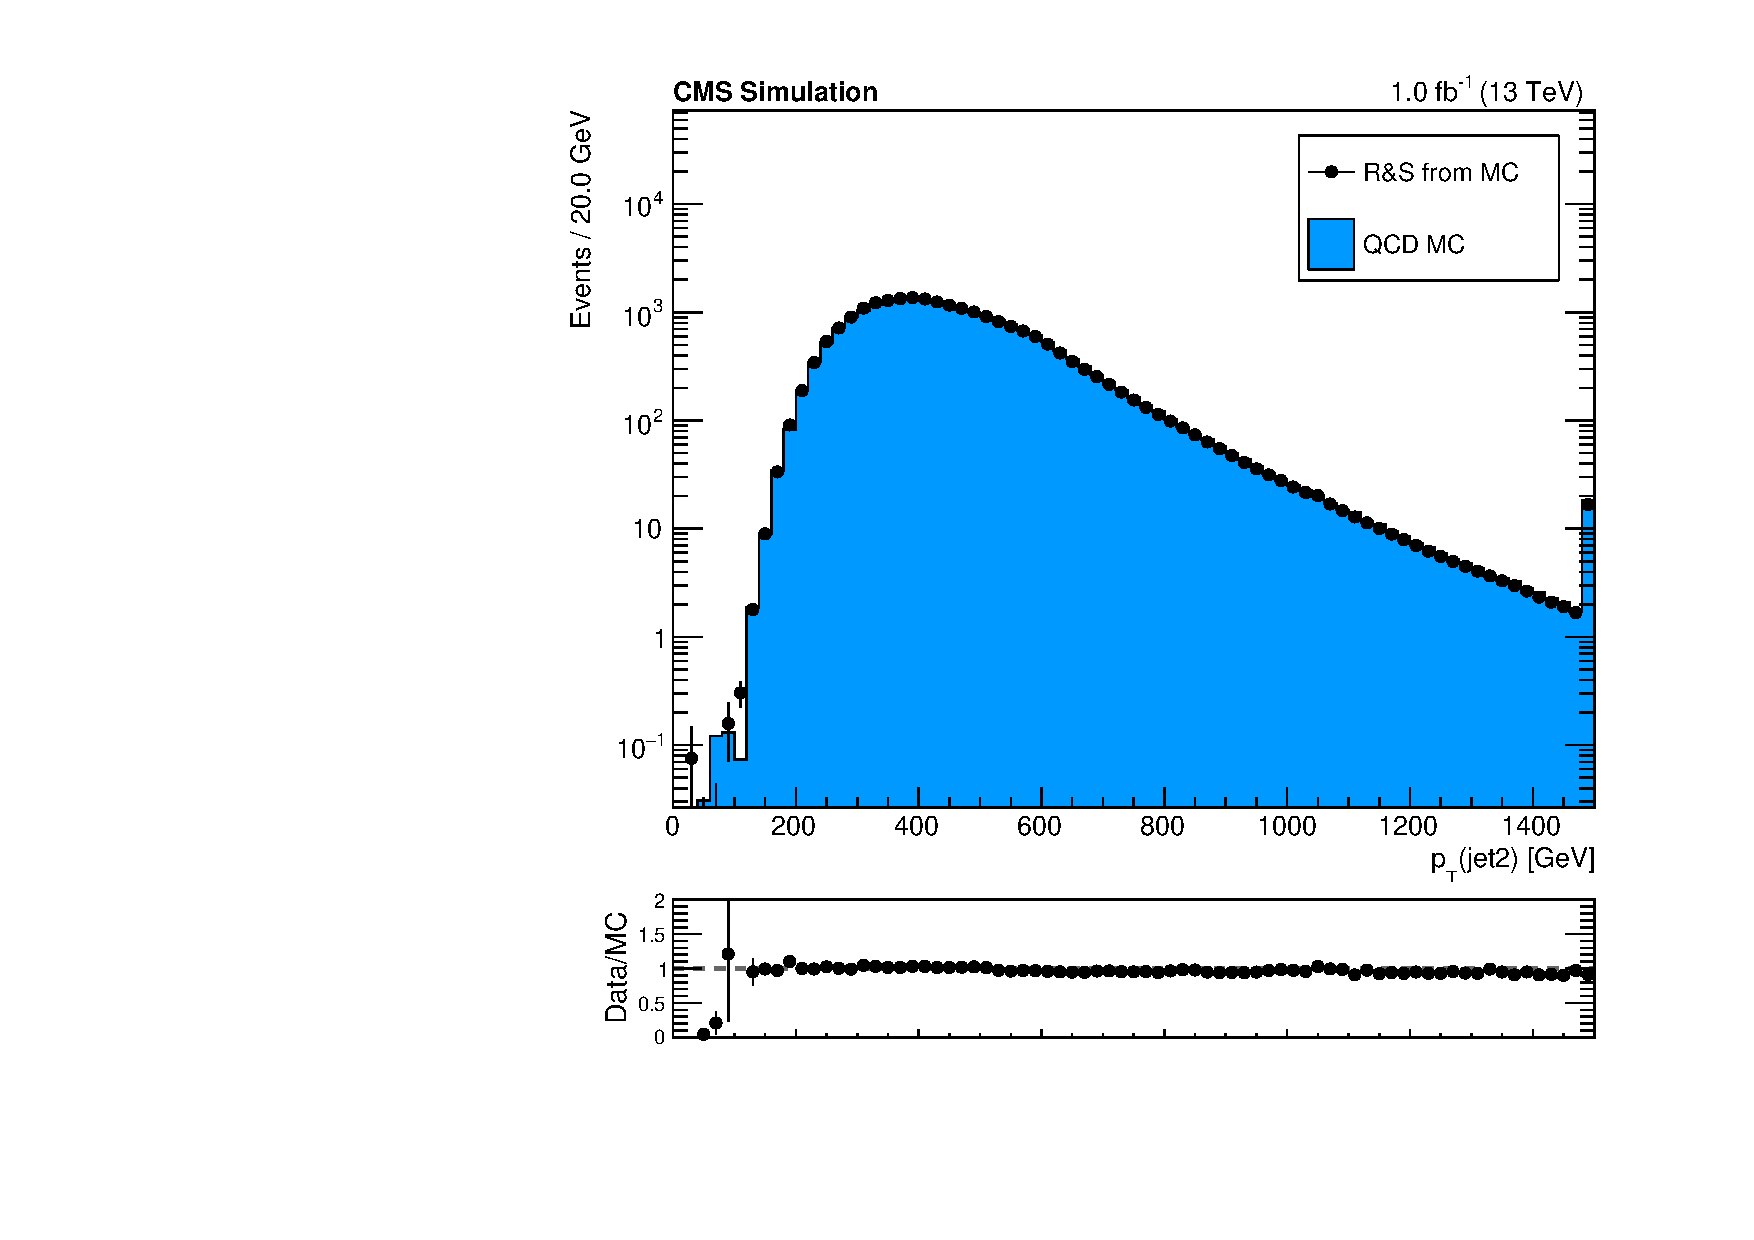
\includegraphics[width=0.46\textwidth]{figs/qcd/rs_mc/highht_J1pt.pdf}
    \caption{\njets, \nbtags and leading- and subleading-jet \pt distributions for Monte Carlo and \rs based on MC. The selection is $\Ht > 1200$\GeV, $\ptmiss > 30$\GeV and $\mttwo > 50$\GeV.
            }
    \label{Fig:rs_mc_jets_highht}
  \end{center}
\end{figure}

\begin{figure}[htbp]
  \begin{center}
    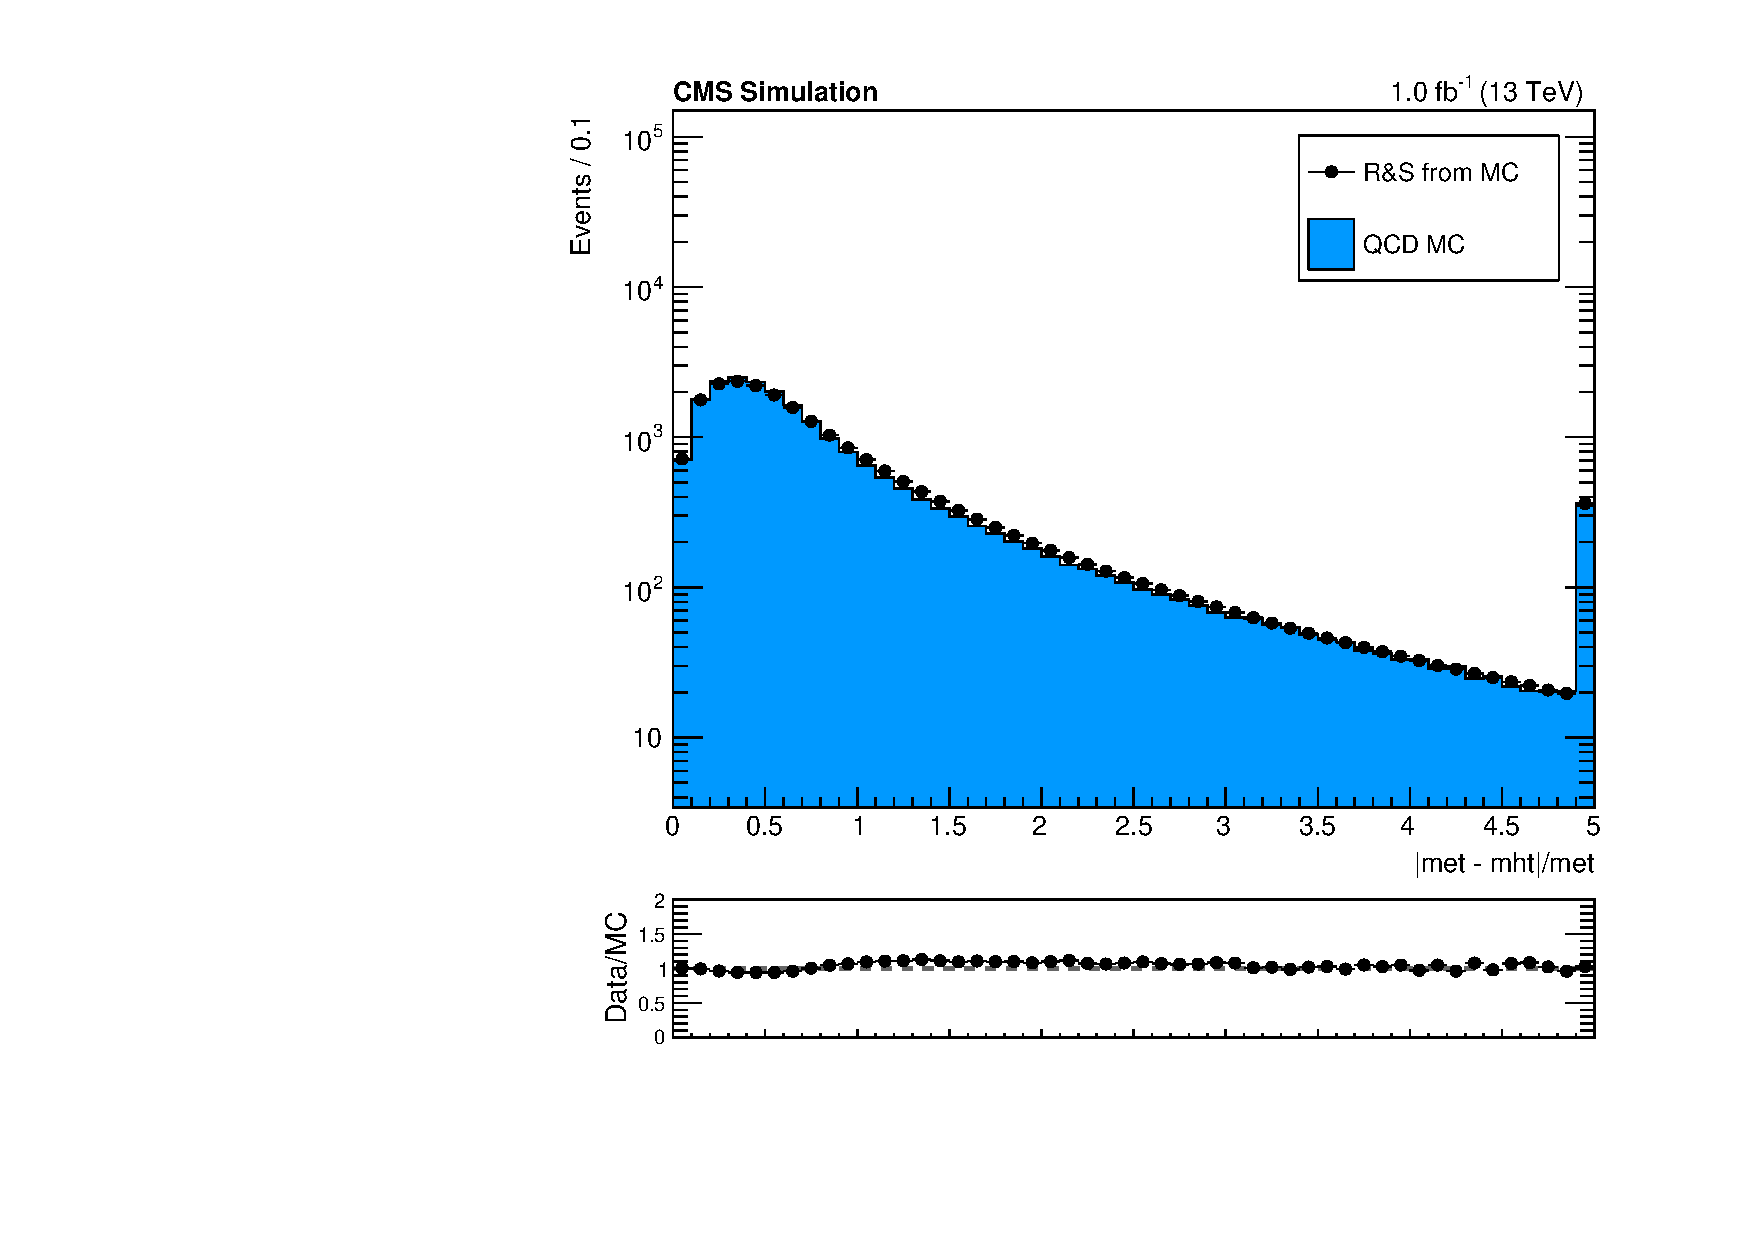
\includegraphics[width=0.46\textwidth]{figs/qcd/rs_mc/highht_diffMetMhtOverMet.pdf}
    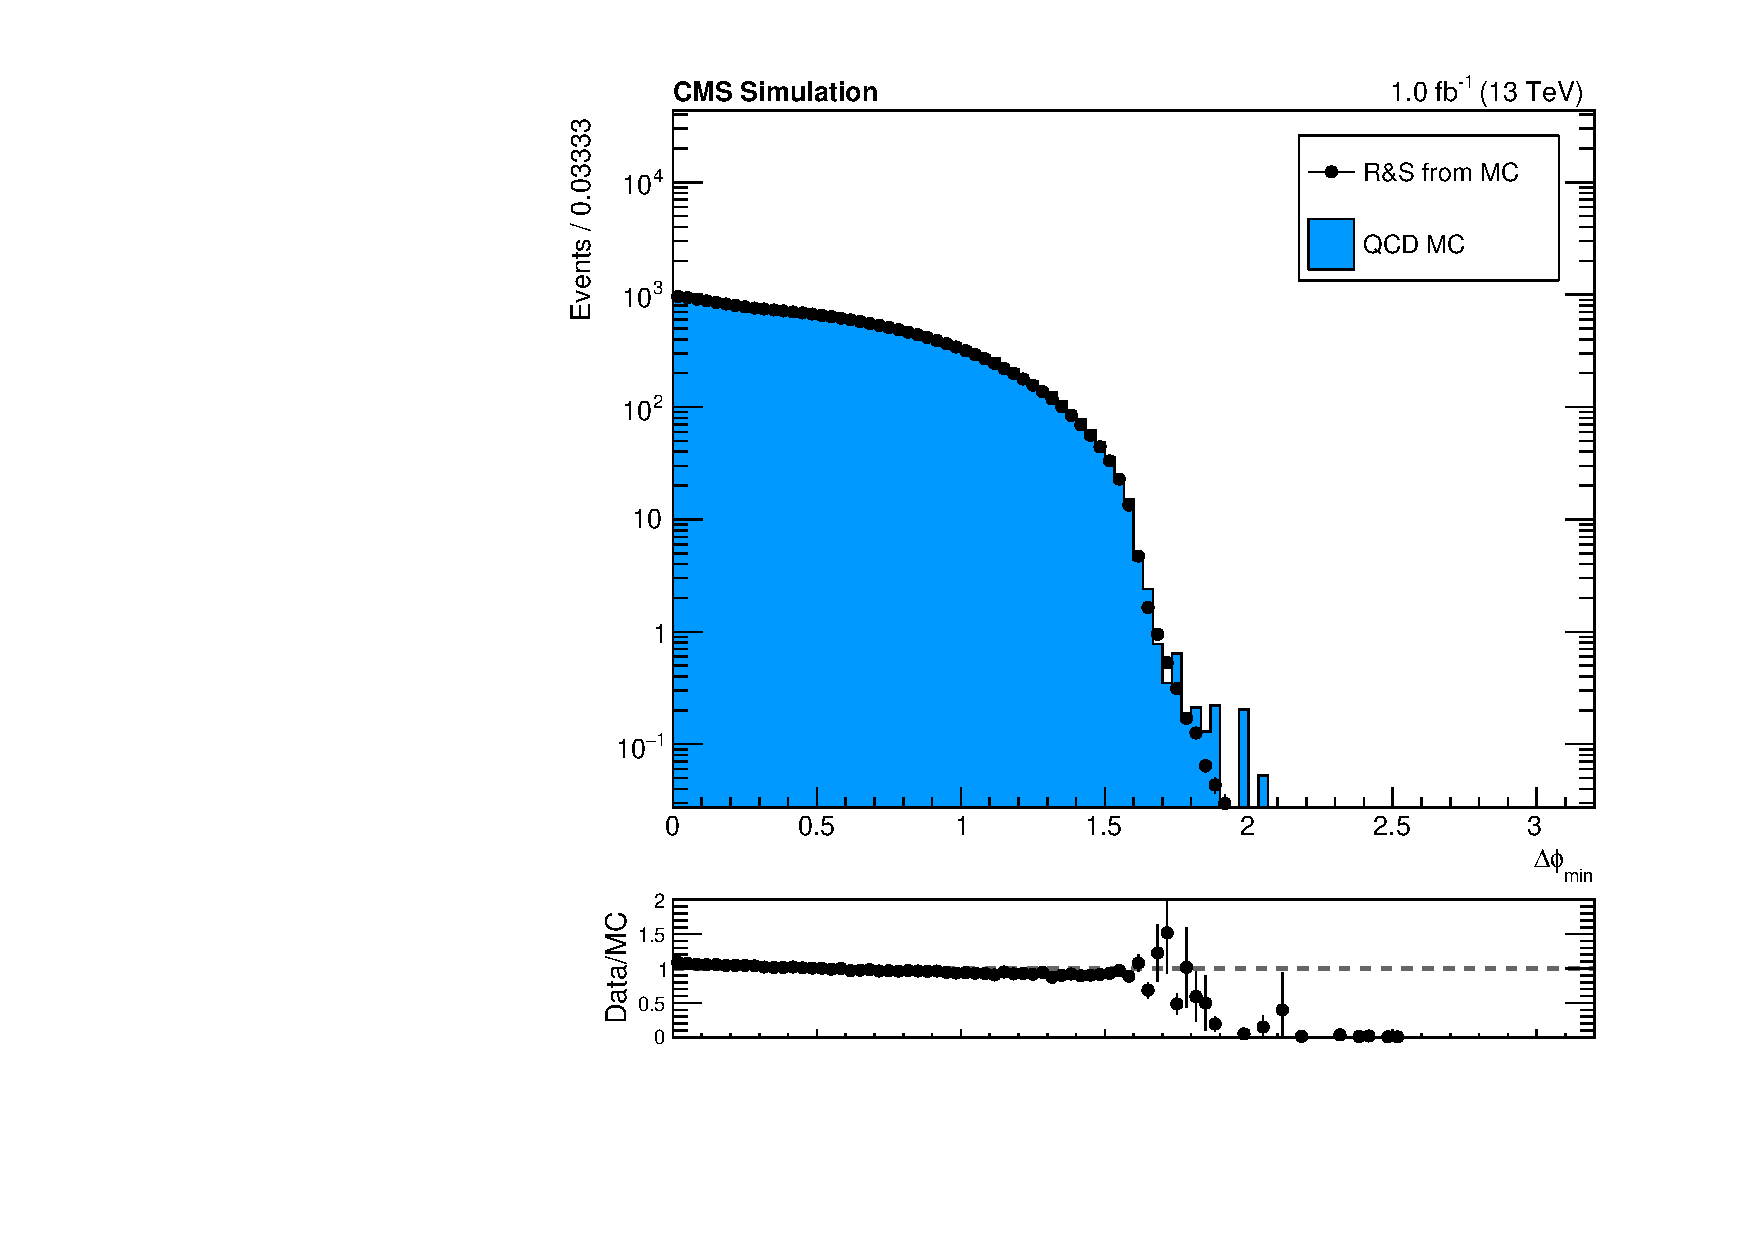
\includegraphics[width=0.46\textwidth]{figs/qcd/rs_mc/highht_deltaPhiMin.pdf}
    \caption{$|\vMht-\vMet|/\ptmiss$ and \dphimet distributions for Monte Carlo and \rs based on MC. The selection is $\Ht > 1200$\GeV, $\ptmiss > 30$\GeV and $\mttwo > 50$\GeV.
            }
    \label{Fig:rs_mc_deltaphi_highht}
  \end{center}
\end{figure}

\begin{figure}[htbp]
  \begin{center}
    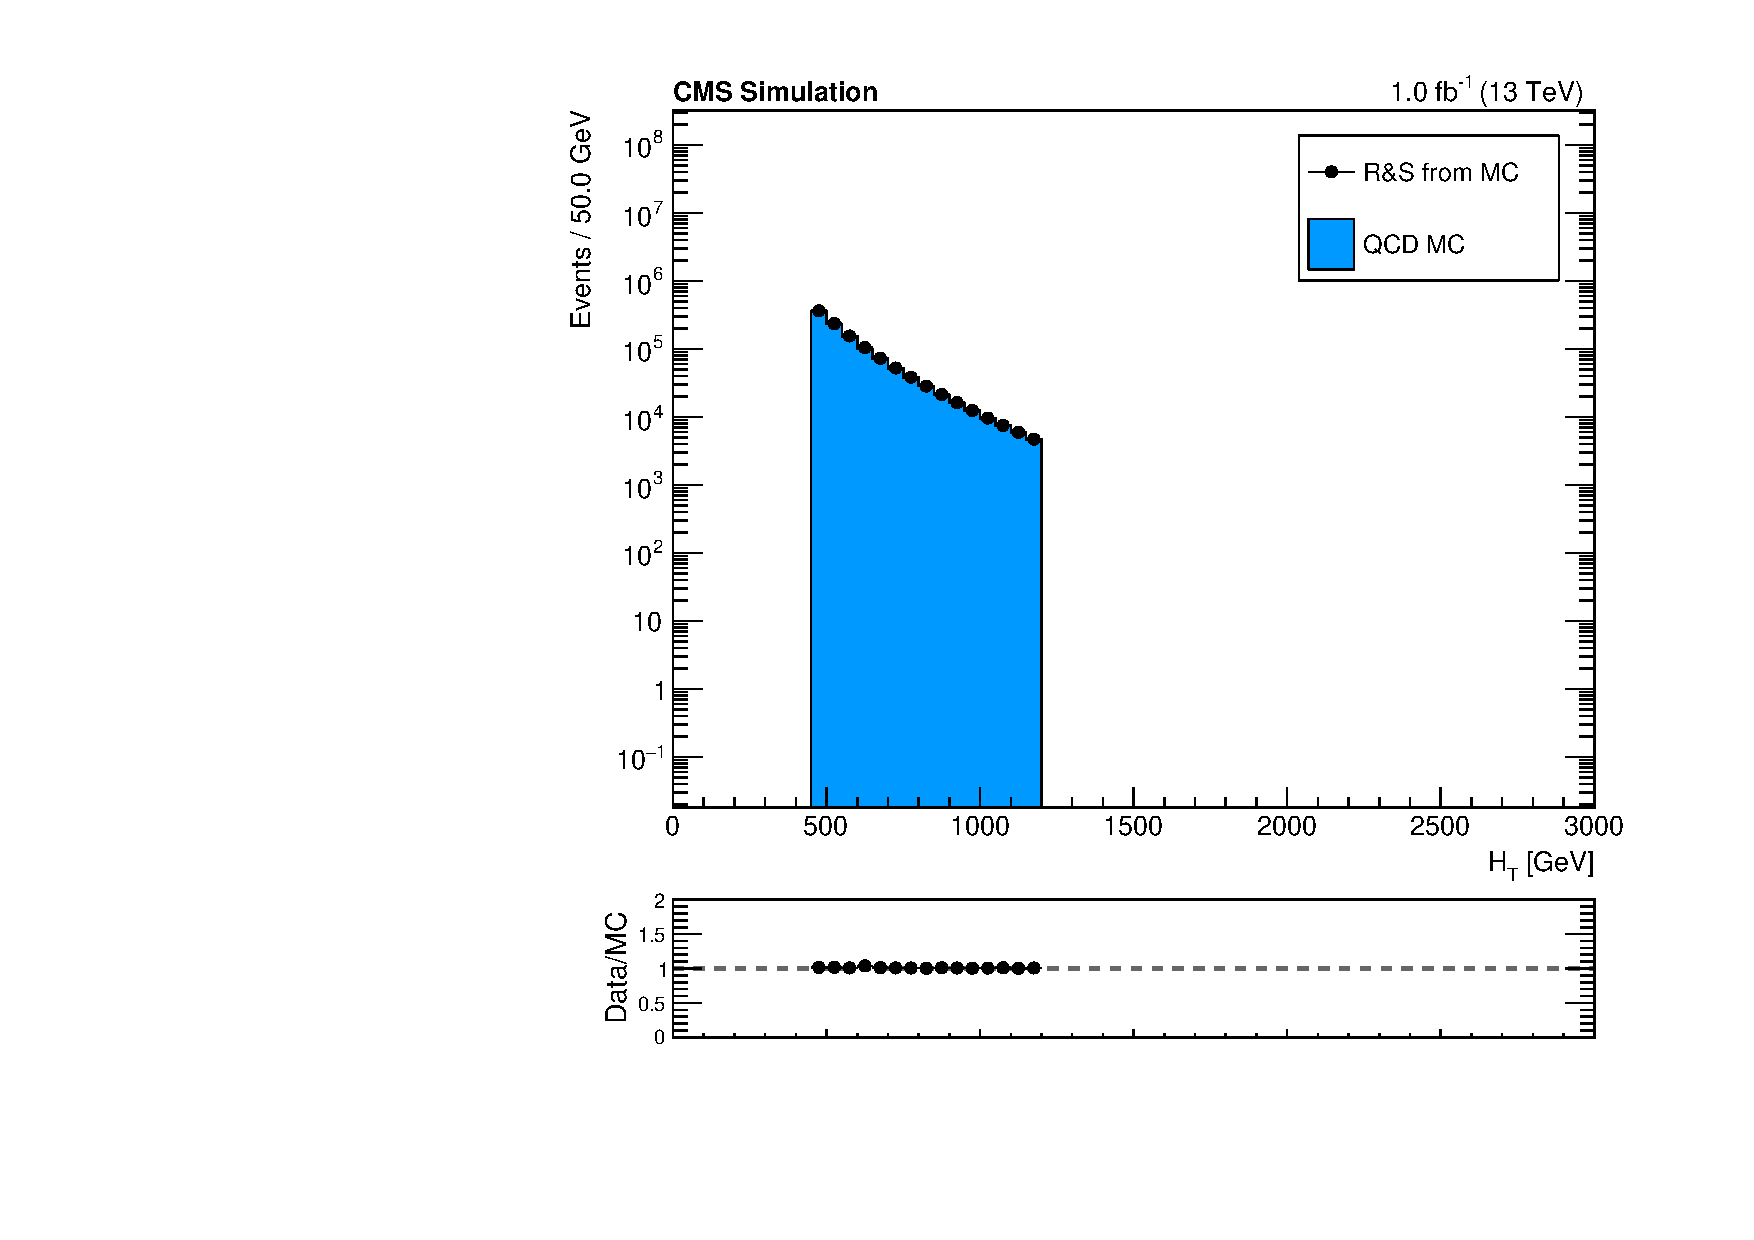
\includegraphics[width=0.46\textwidth]{figs/qcd/rs_mc/lowht_ht.pdf}
    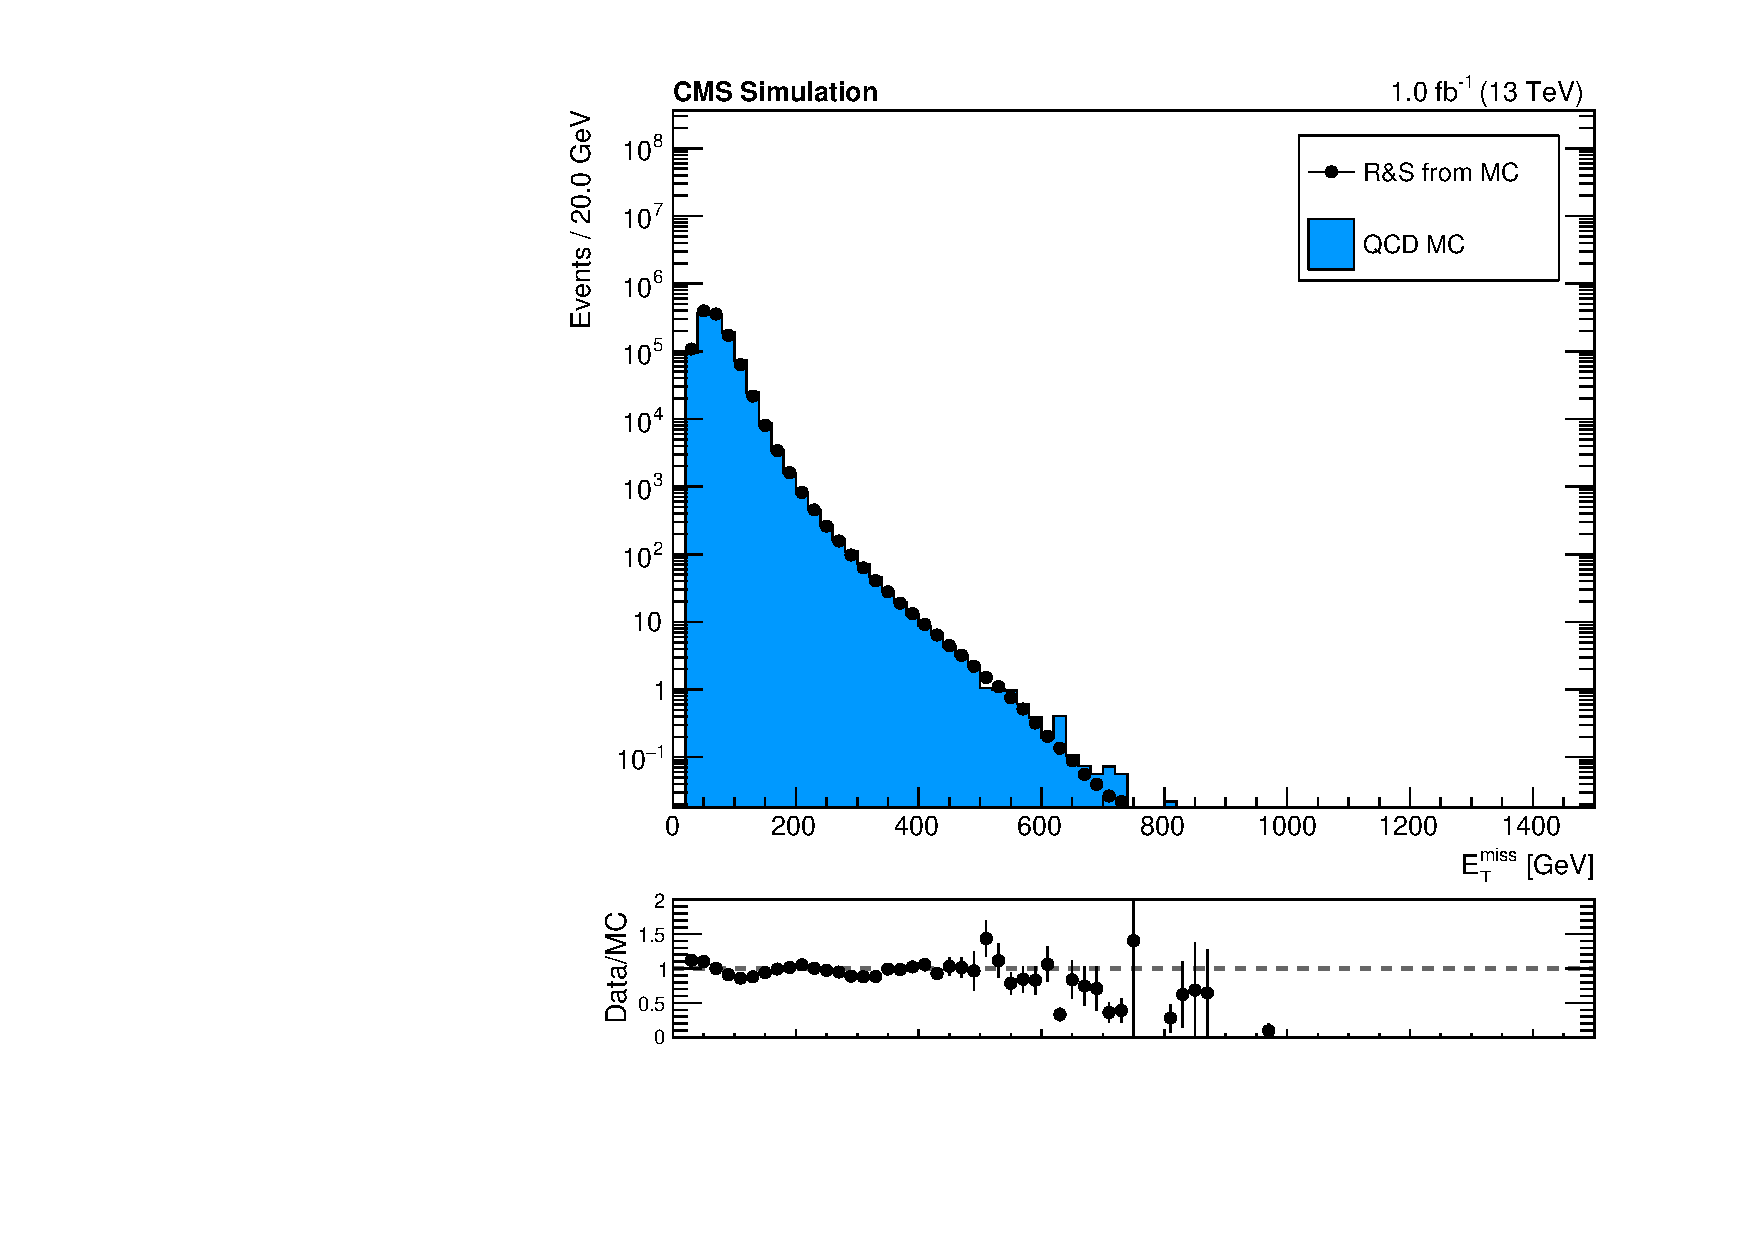
\includegraphics[width=0.46\textwidth]{figs/qcd/rs_mc/lowht_met.pdf} \\
    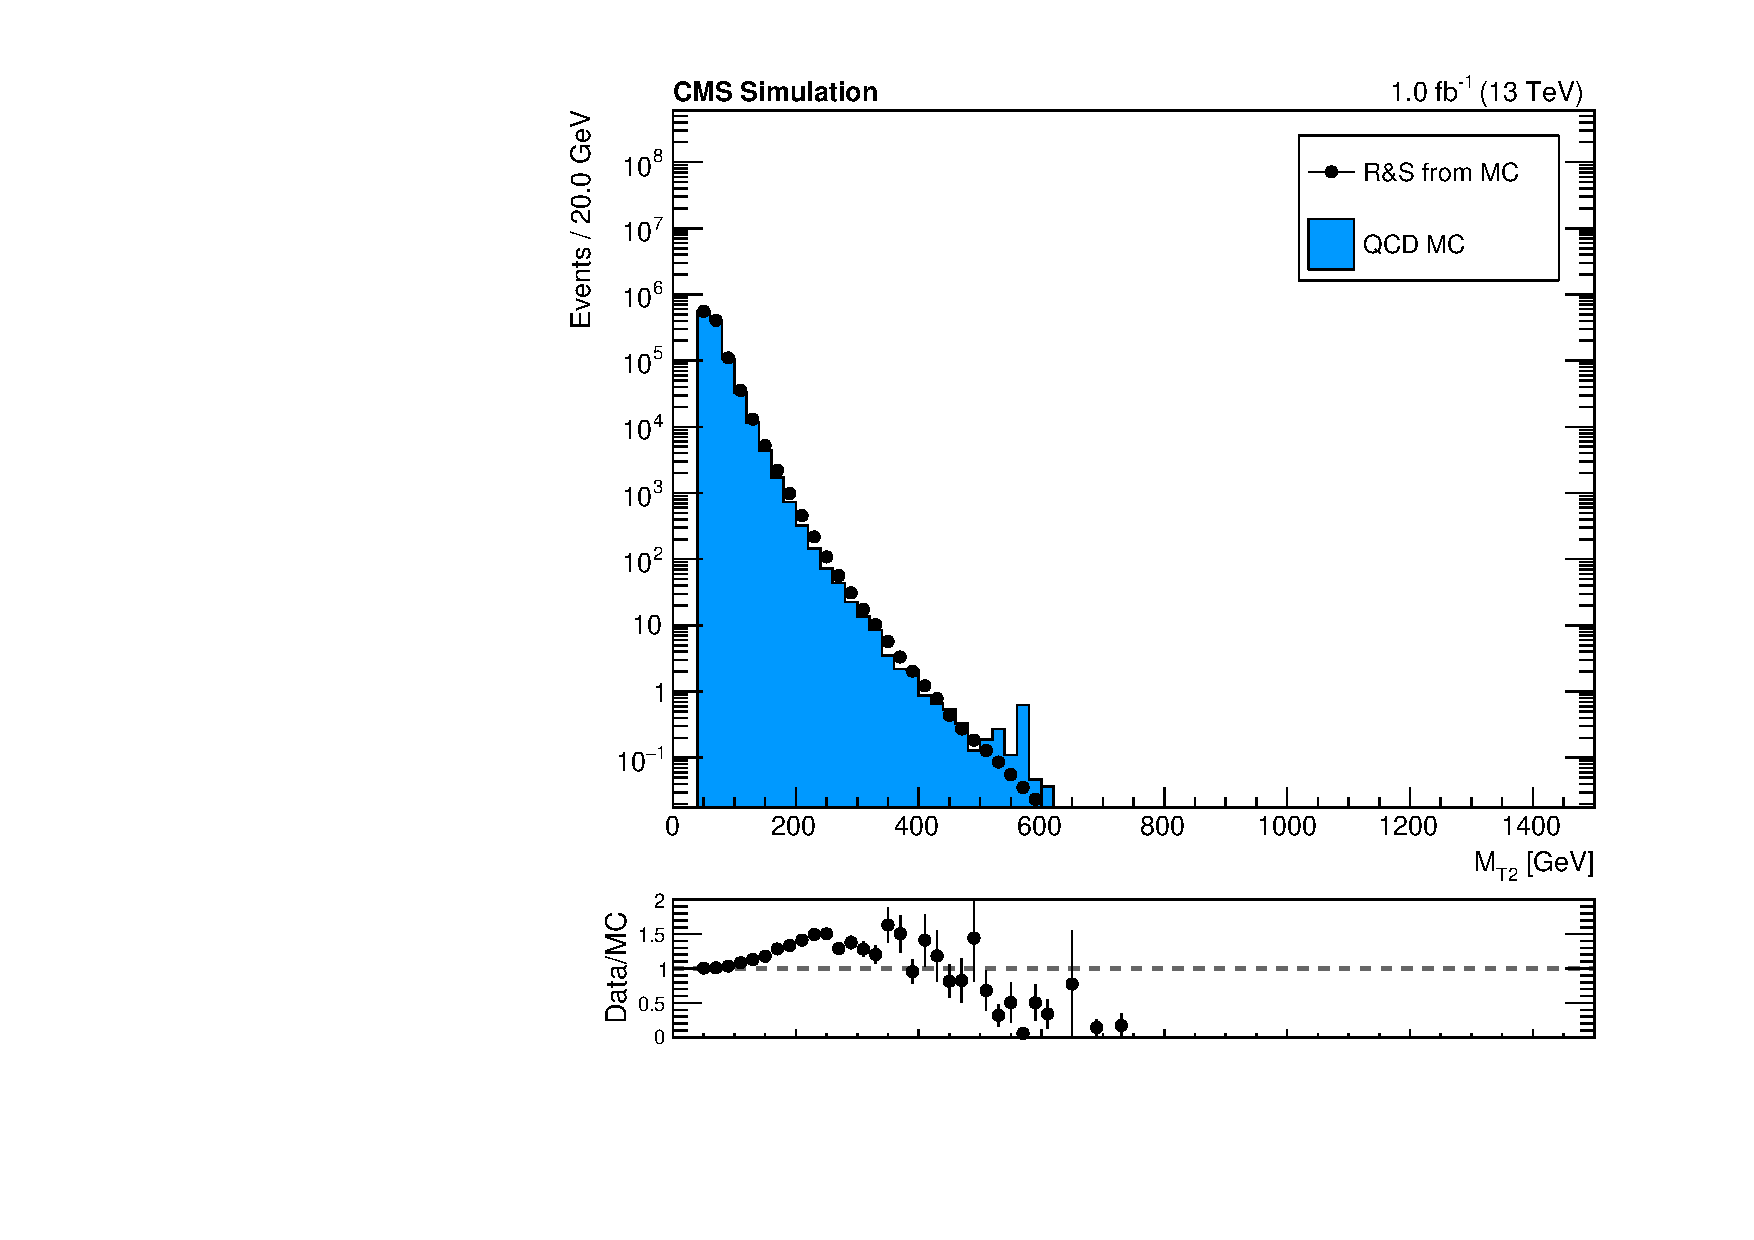
\includegraphics[width=0.46\textwidth]{figs/qcd/rs_mc/lowht_mt2.pdf}
    \caption{\Ht, \ptmiss, and \mttwo distributions for Monte Carlo and \rs based on MC. The selection is $450 < \Ht < 1200$\GeV, $\ptmiss > 30$\GeV and $\mttwo > 50$\GeV.
            }
    \label{Fig:rs_mc_ht_met_lowht}
  \end{center}
\end{figure}

\begin{figure}[htbp]
  \begin{center}
    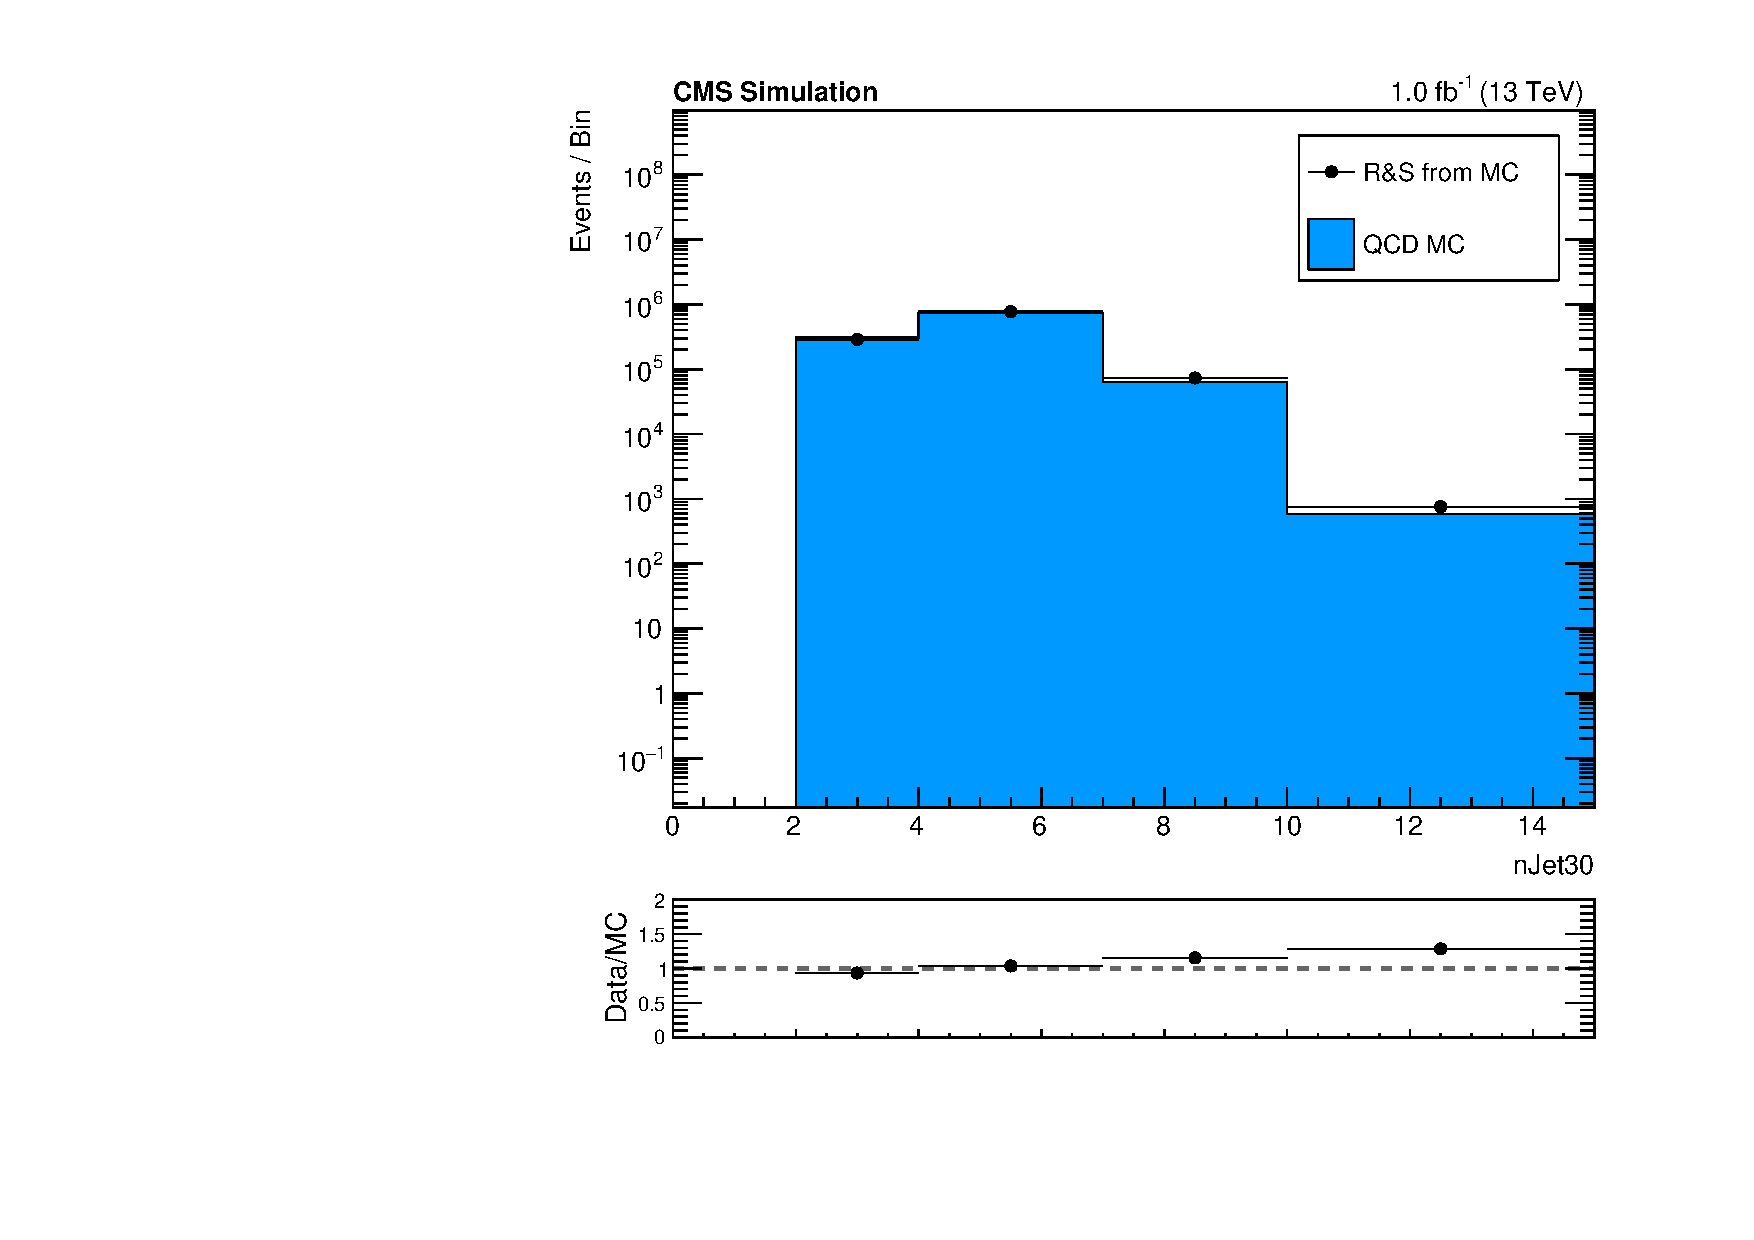
\includegraphics[width=0.46\textwidth]{figs/qcd/rs_mc/lowht_nJet30.pdf}
    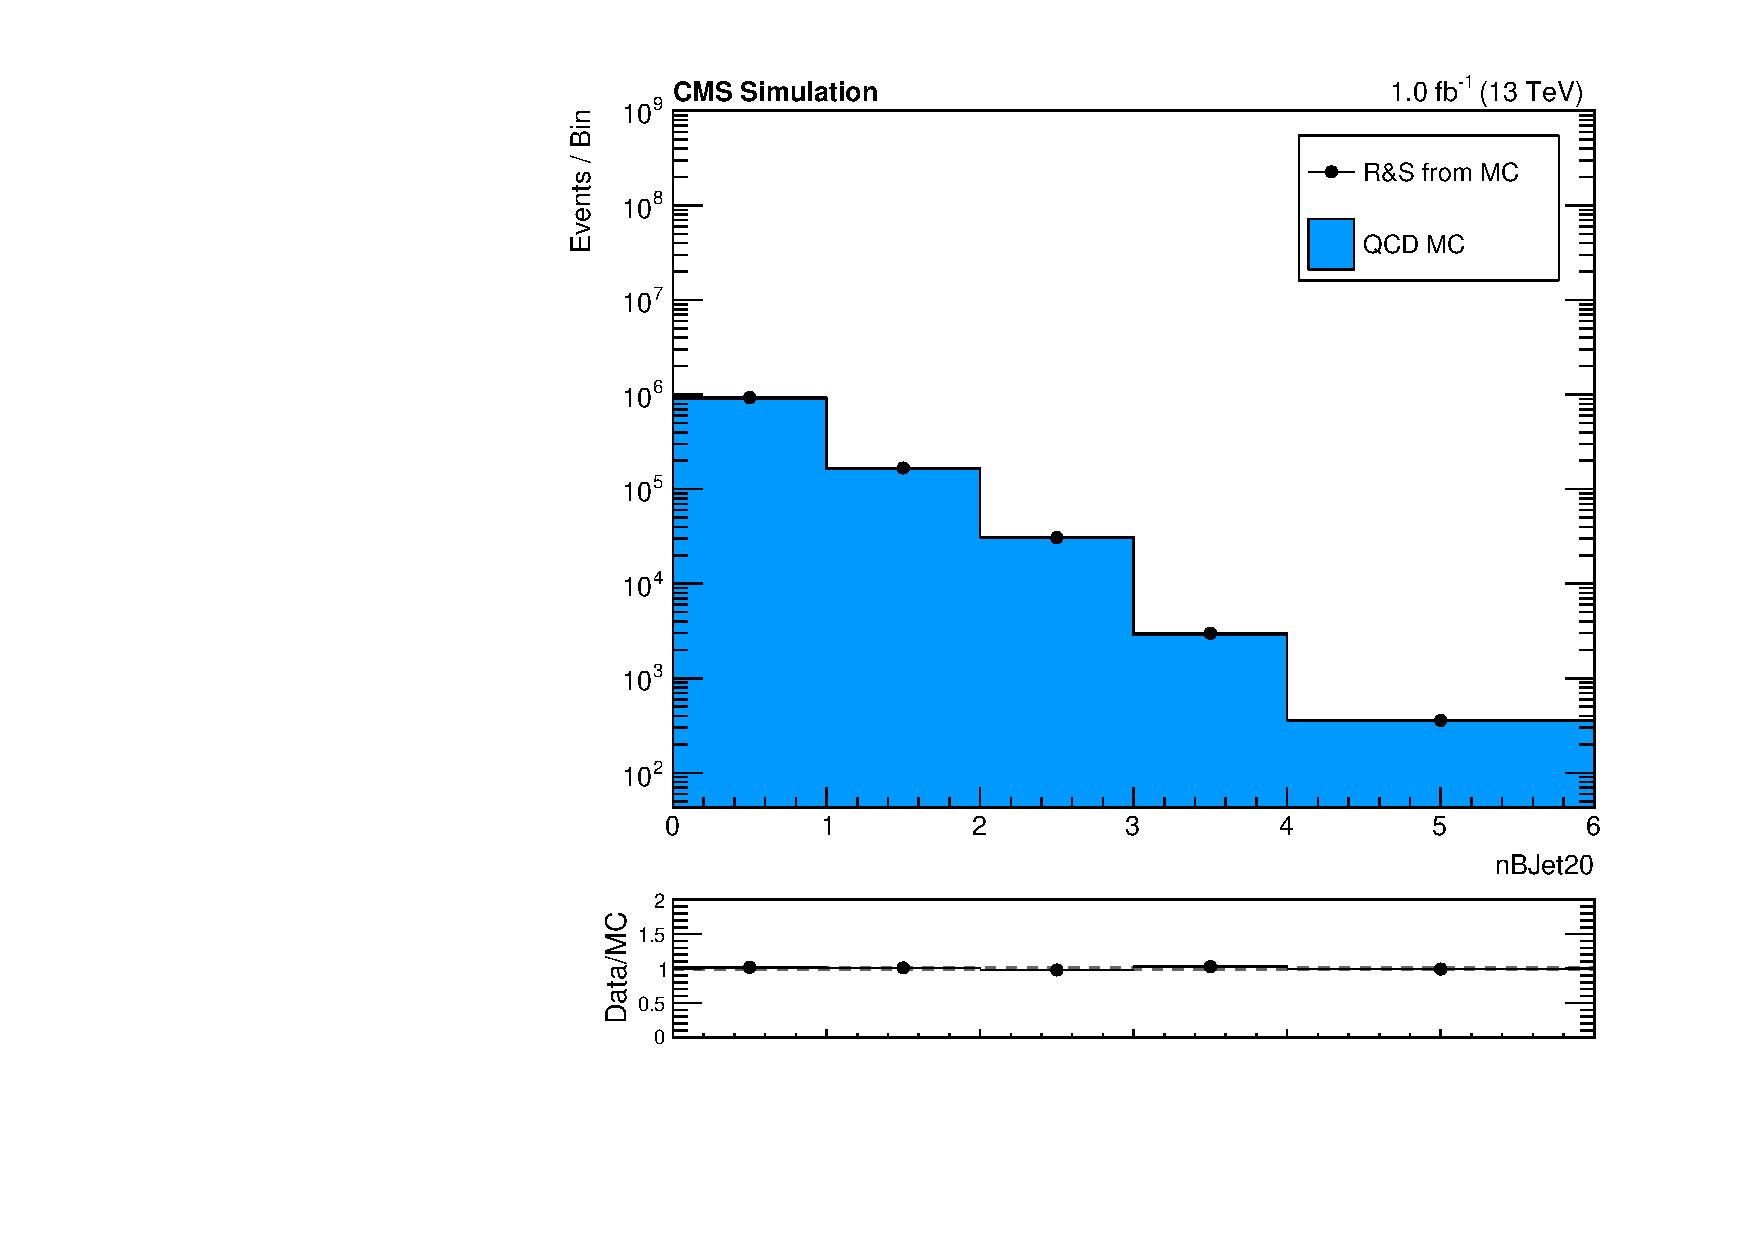
\includegraphics[width=0.46\textwidth]{figs/qcd/rs_mc/lowht_nBJet20.pdf} \\
    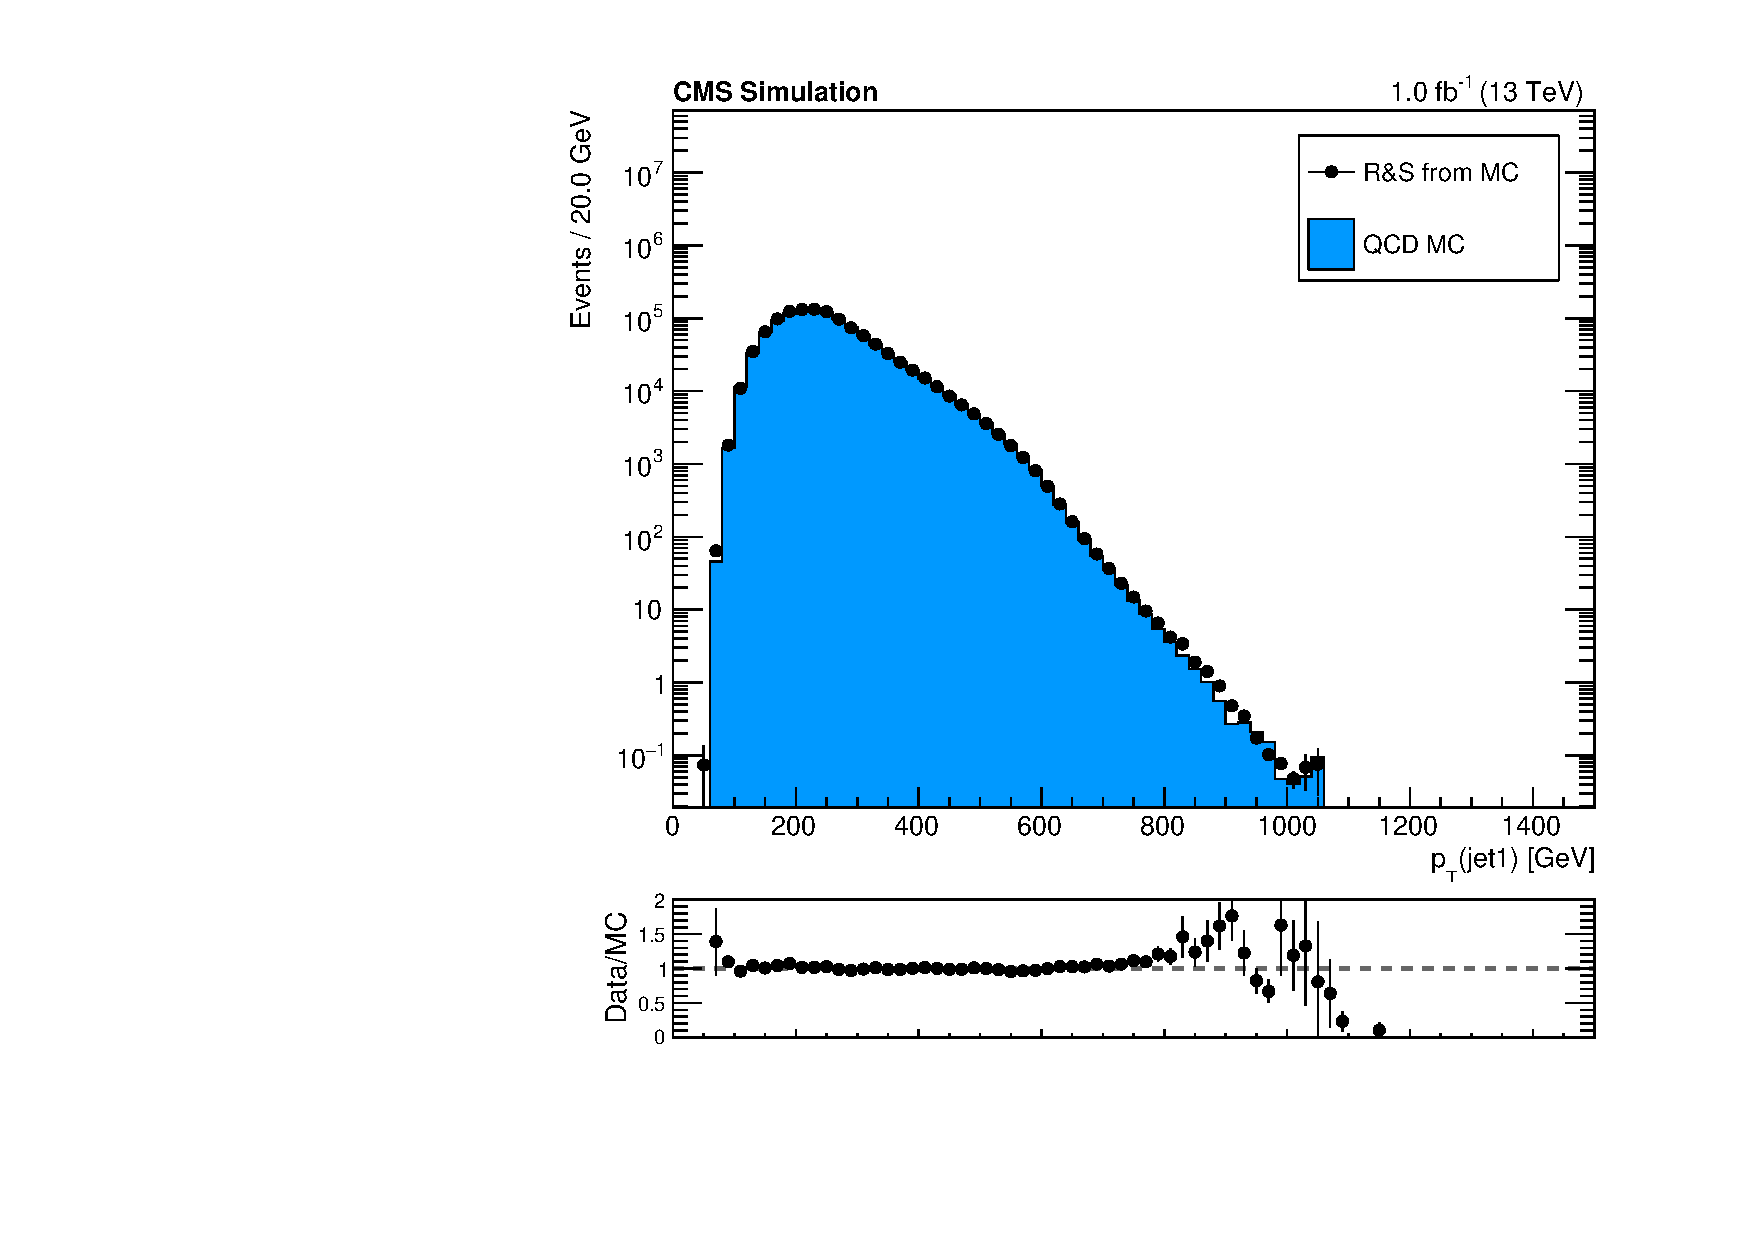
\includegraphics[width=0.46\textwidth]{figs/qcd/rs_mc/lowht_J0pt.pdf}
    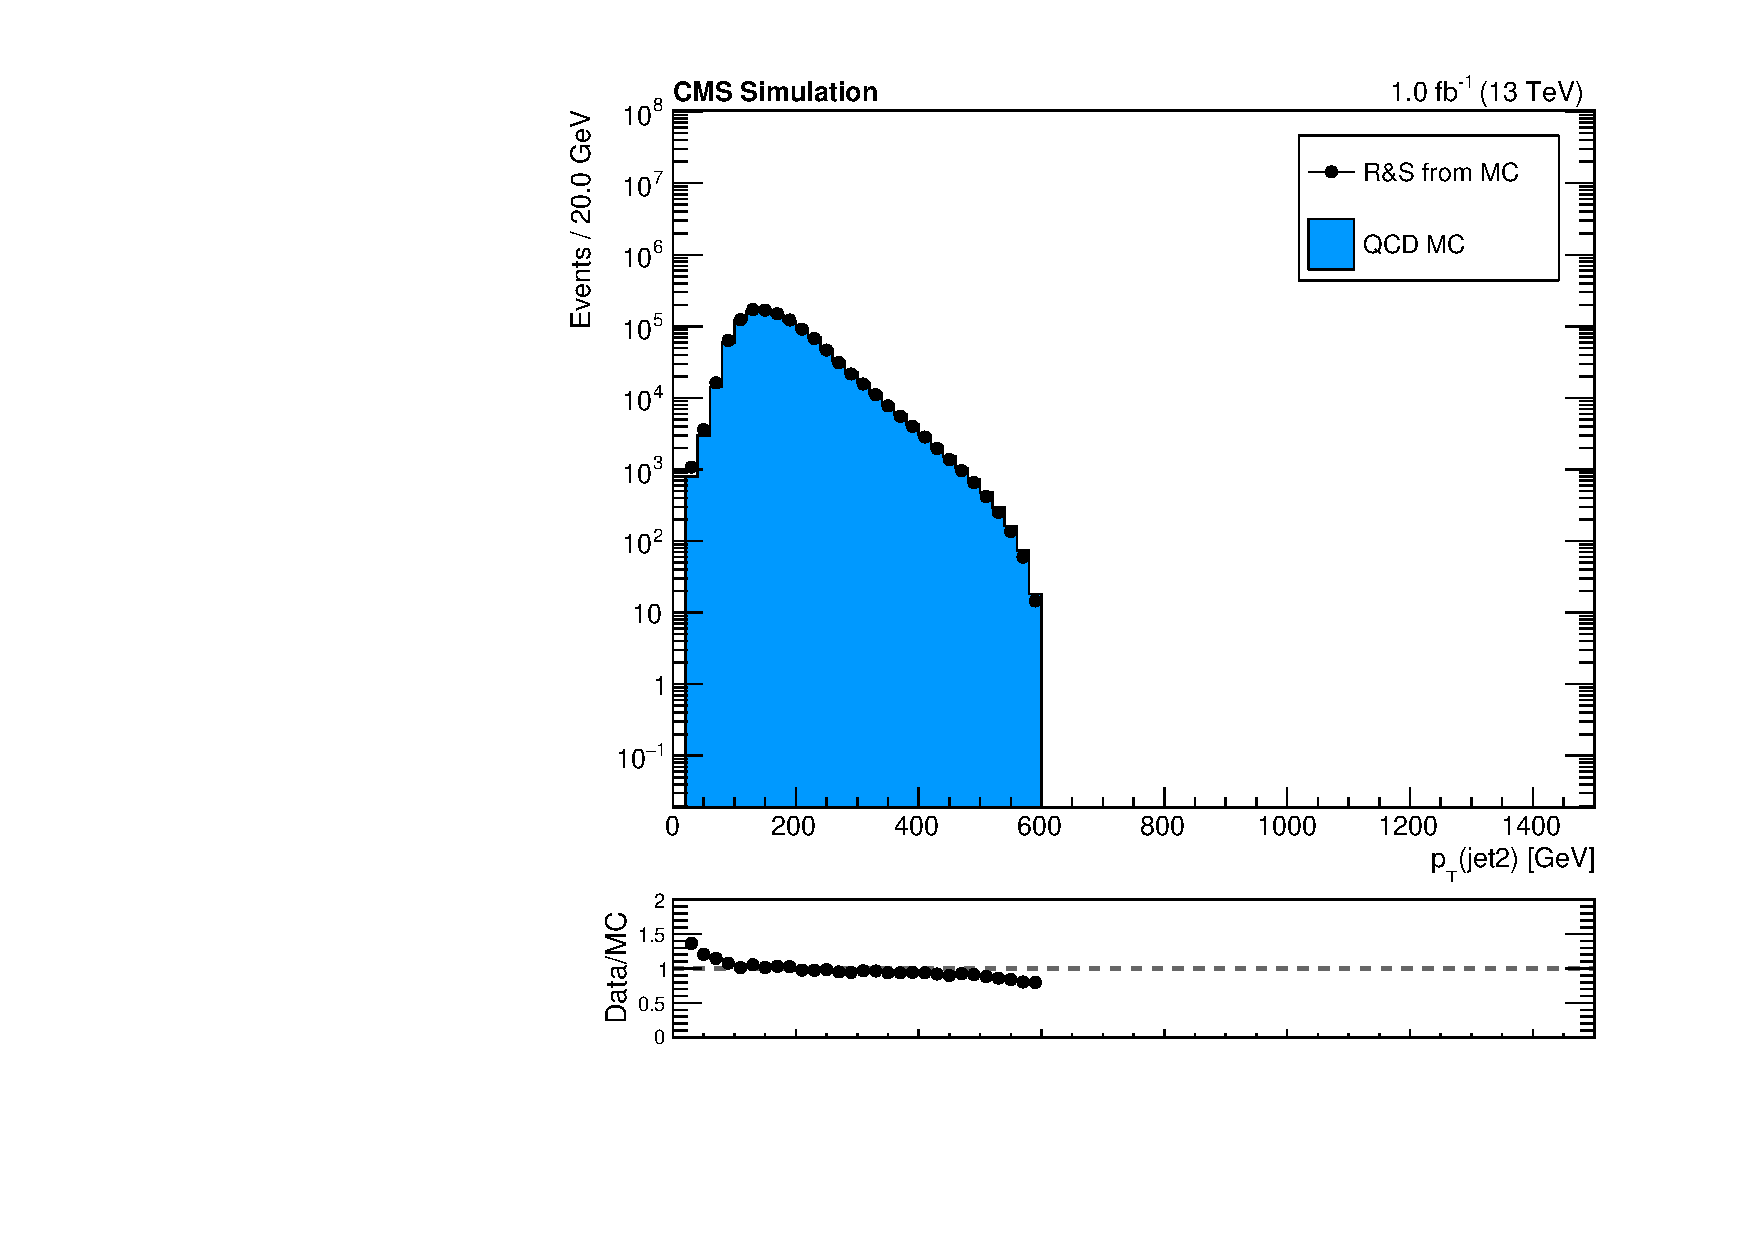
\includegraphics[width=0.46\textwidth]{figs/qcd/rs_mc/lowht_J1pt.pdf}
    \caption{\njets, \nbtags and leading- and subleading-jet \pt distributions for Monte Carlo and \rs based on MC. The selection is $450 < \Ht < 1200$\GeV, $\ptmiss > 30$\GeV and $\mttwo > 50$\GeV.
            }
    \label{Fig:rs_mc_jets_lowht}
  \end{center}
\end{figure}

\begin{figure}[htbp]
  \begin{center}
    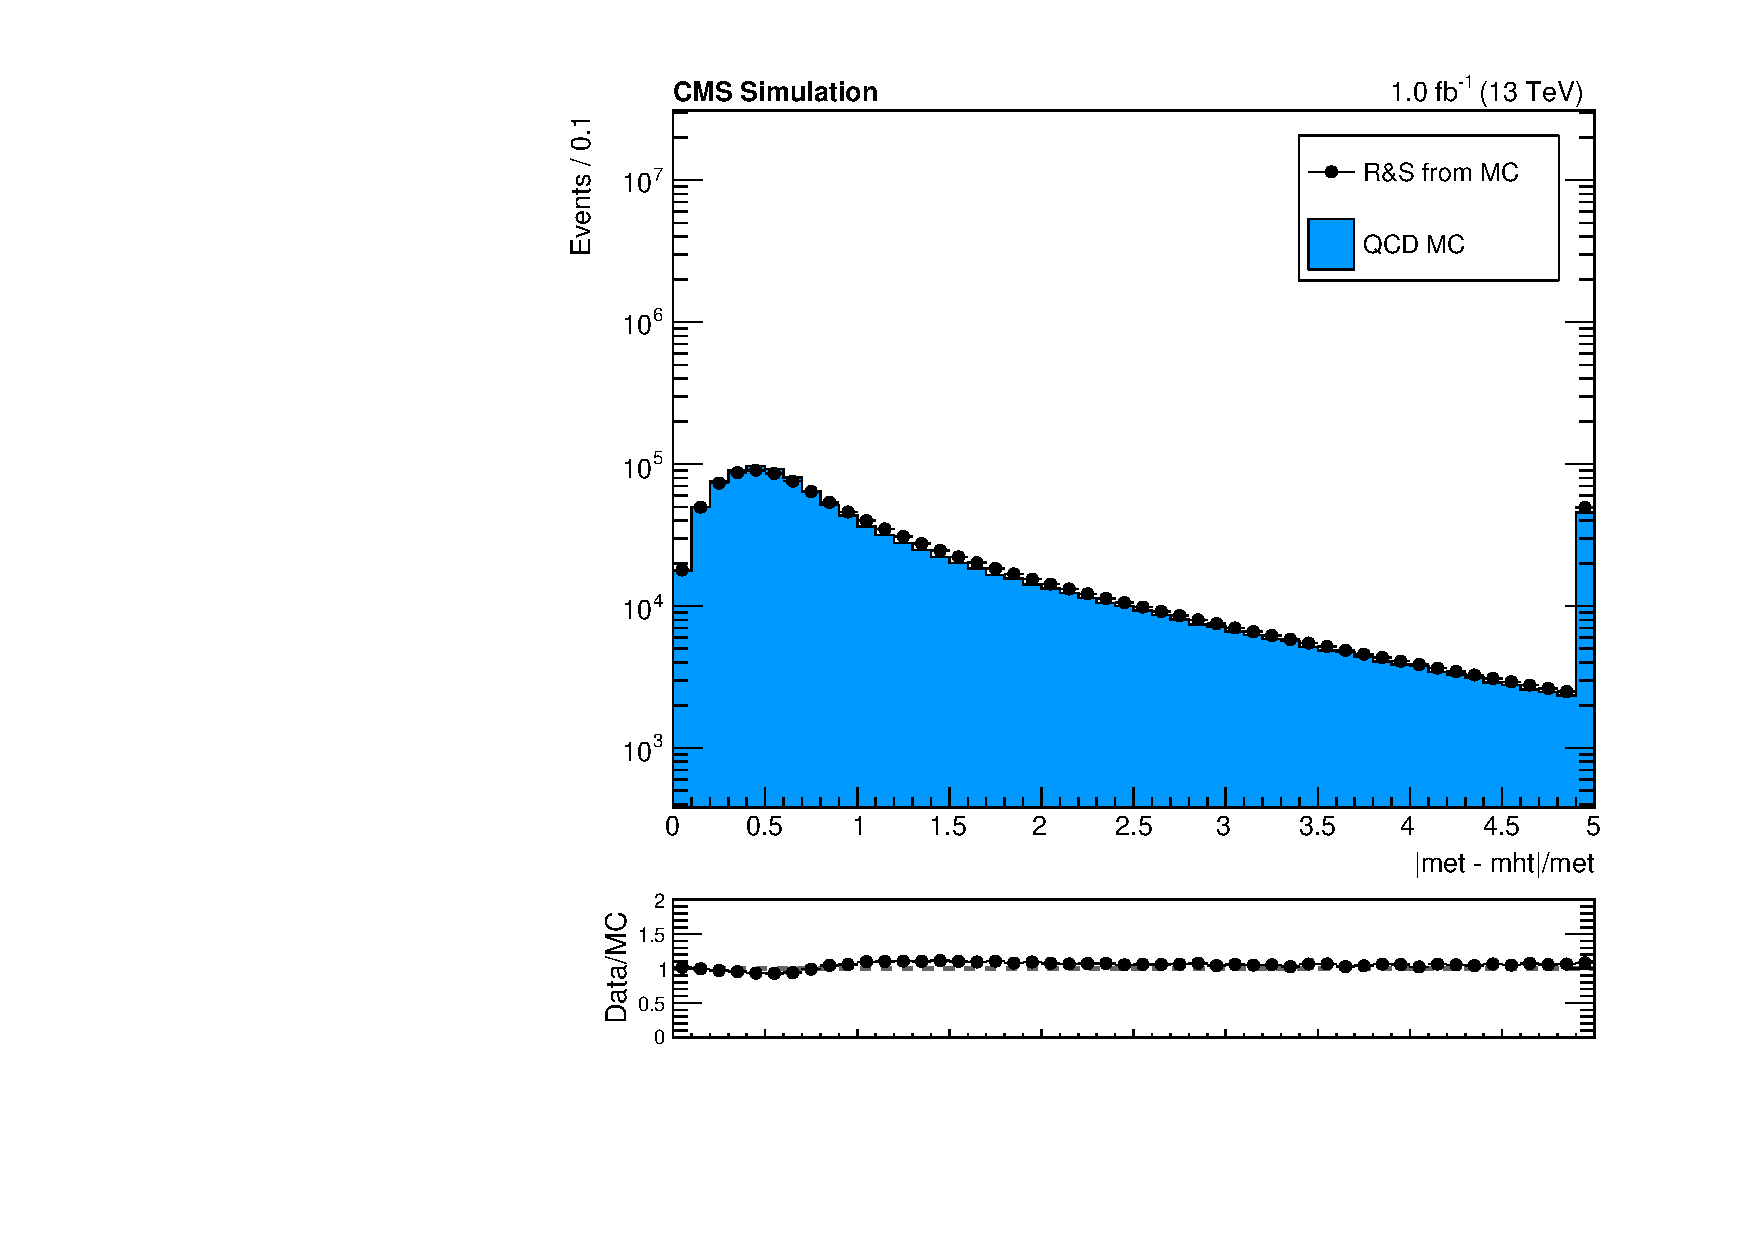
\includegraphics[width=0.46\textwidth]{figs/qcd/rs_mc/lowht_diffMetMhtOverMet.pdf}
    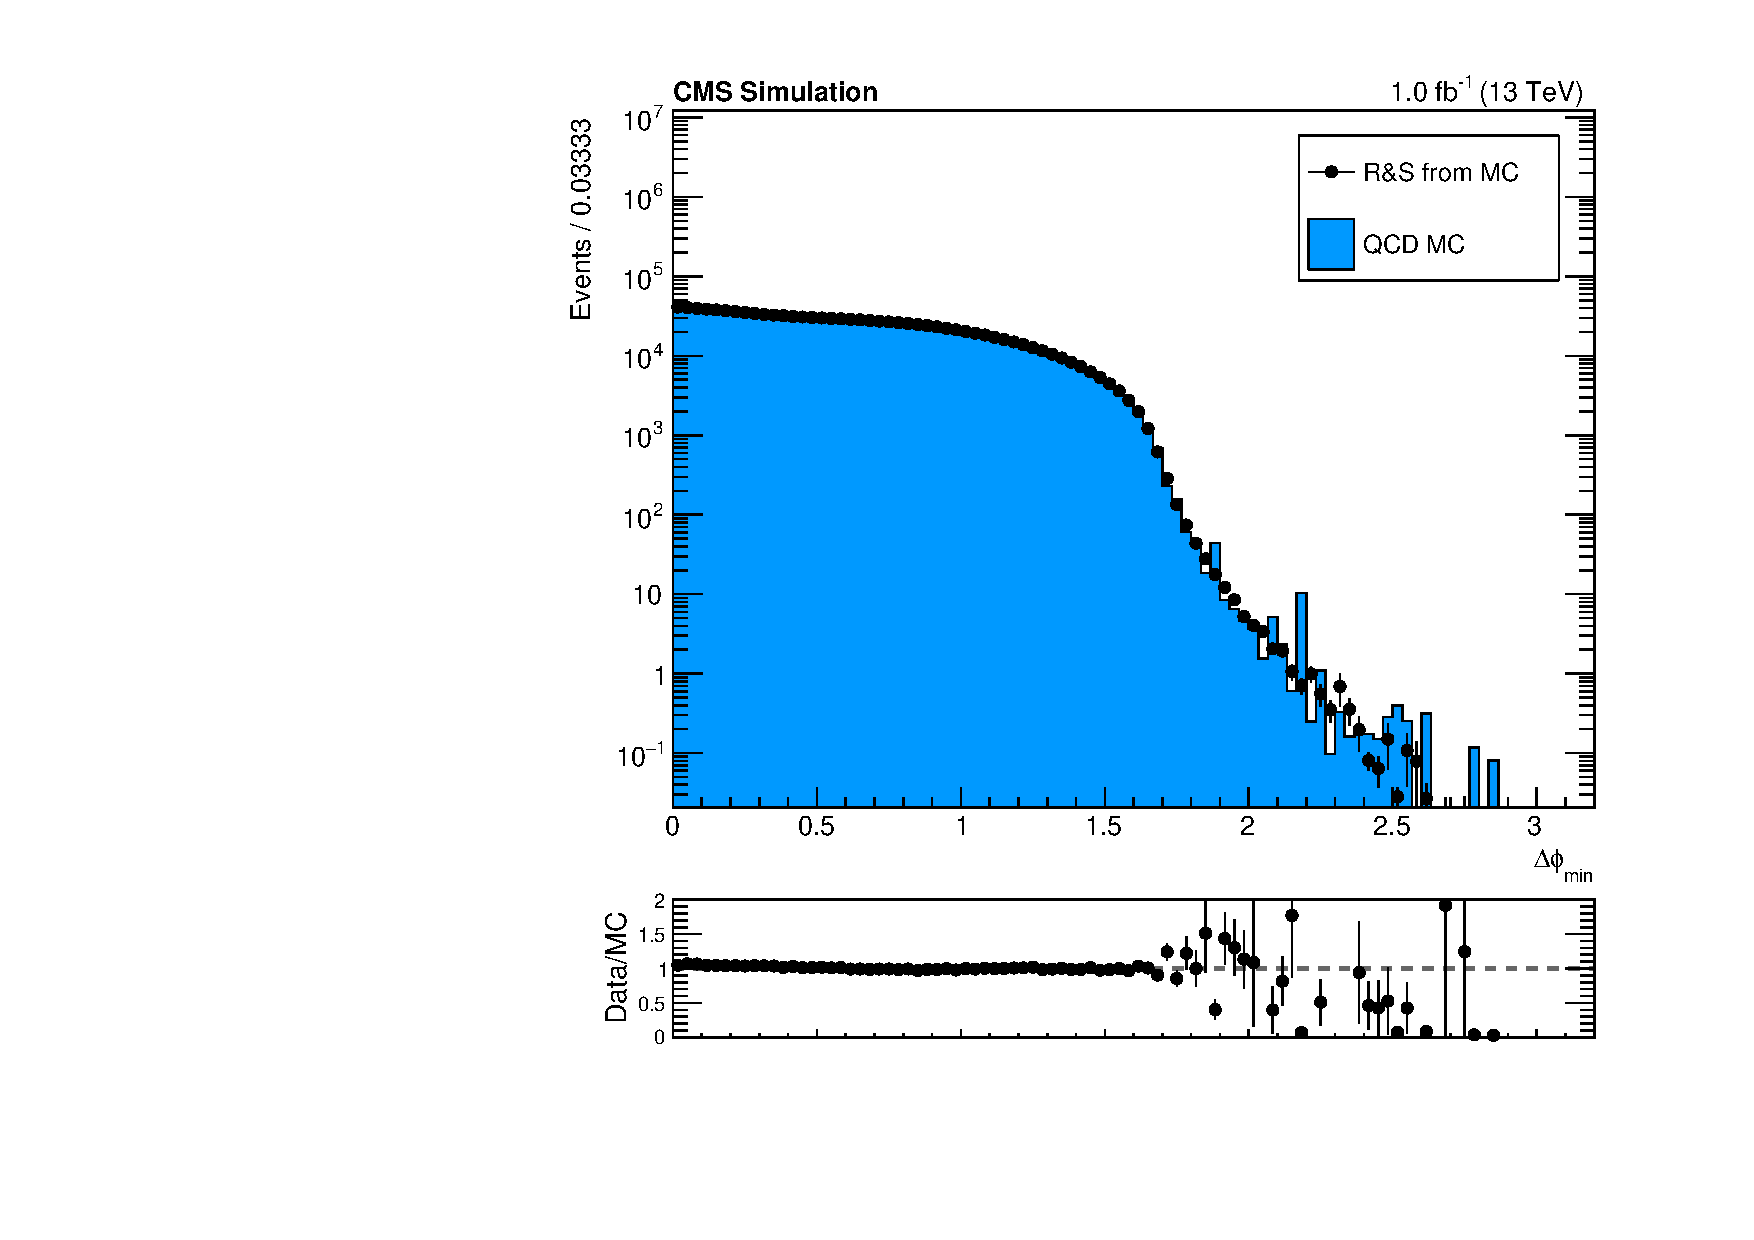
\includegraphics[width=0.46\textwidth]{figs/qcd/rs_mc/lowht_deltaPhiMin.pdf}
    \caption{$|\vMht-\vMet|/\ptmiss$ and \dphimet distributions for Monte Carlo and \rs based on MC. The selection is $450 < \Ht < 1200$\GeV, $\ptmiss > 30$\GeV and $\mttwo > 50$\GeV.
            }
    \label{Fig:rs_mc_deltaphi_lowht}
  \end{center}
\end{figure}

\begin{figure}[htbp]
  \begin{center}
    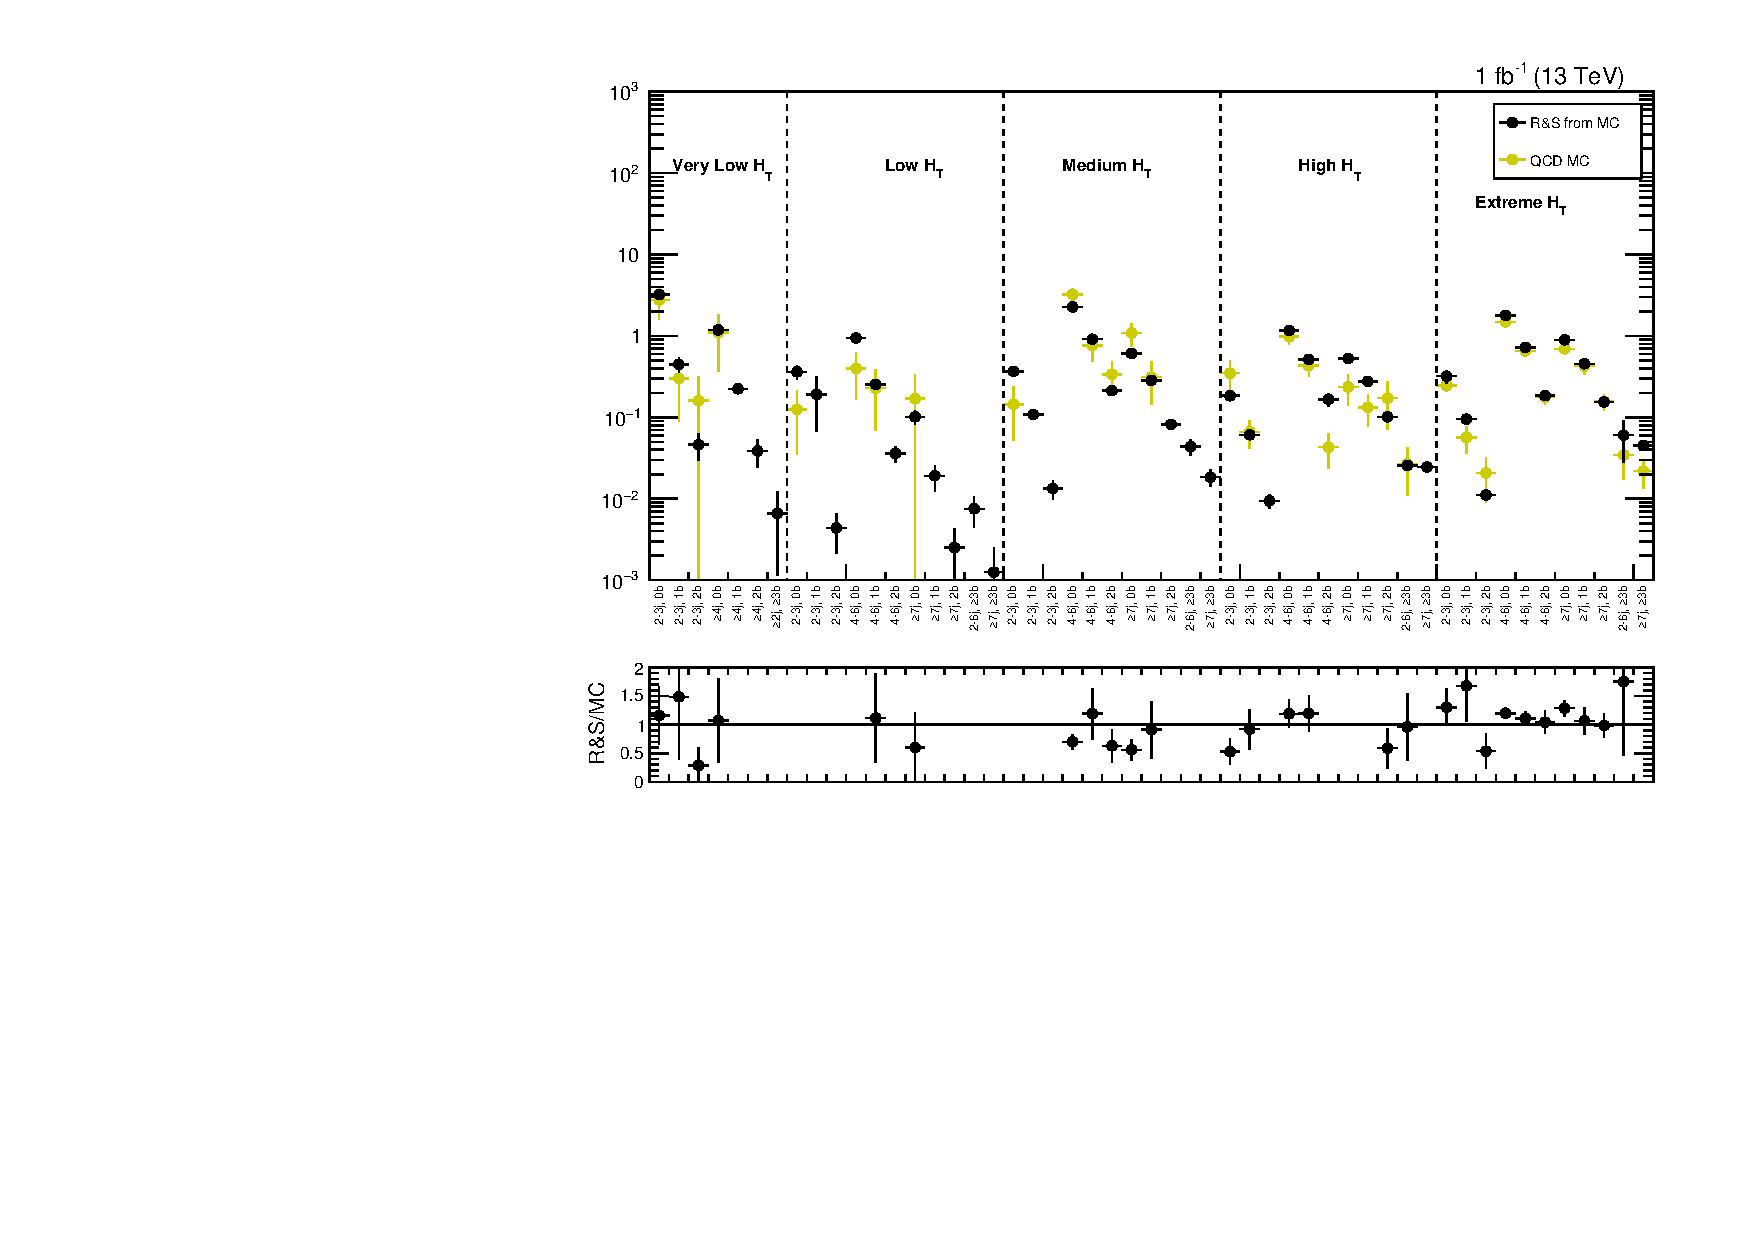
\includegraphics[width=1.0\textwidth]{figs/qcd/rs_mc/mc_comp_sr_ratio.pdf}
    \caption{\rs Monte Carlo closure in topological regions after the baseline signal region selection. The bottom histogram shows the ratio of yields in each region.
            }
    \label{Fig:rs_mc_comp_sr_ratio}
  \end{center}
\end{figure}

\clearpage
\section{Electroweak contamination}
The input to the rebalancing step in data comes from pure-\Ht triggers with no attempt to remove any possible contamination from non-QCD processes. Most electroweak events
are rebalanced to have \ptmiss close to zero just like actual QCD events, and contribute an extremely small amount to the final prediction since the cross section for electroweak processes
is much smaller than the QCD cross section. However, some configurations of electroweak events prove difficult to rebalance, such as events with \ptmiss in one hemisphere and all
jets in the other hemisphere. An example of one such Monte Carlo event is shown in Figure ~\ref{Fig:rs_ewk_zinv_event} The \ptmiss in these events is reduced in the rebalancing step
but can still be rather large. When the \ptmiss after rebalancing is large, almost all smeared events will also have large \ptmiss and will therefore contribute to the final prediction
much more than if the smeared \ptmiss was actually a product of sampling the tails of the jet response templates.

\begin{figure}[htbp]
  \begin{center}
    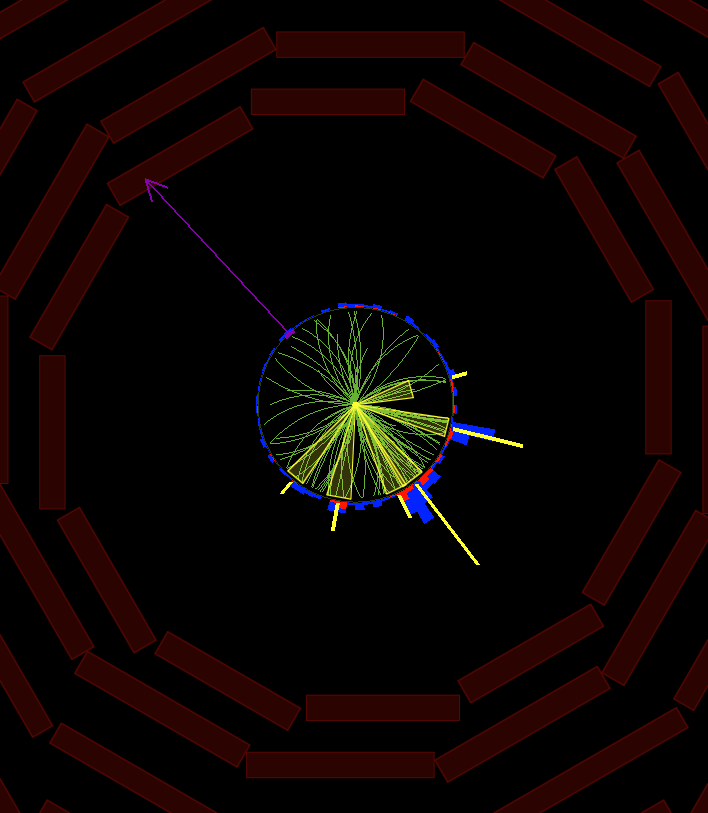
\includegraphics[width=0.46\textwidth]{figs/qcd/rs_mc/ewk/zinv_ht400to600_met500_njet6.png}
    \caption{Example of a \znunu event in Monte Carlo with a configuration that leads to large \ptmiss after rebalancing.
             This event has 517\GeV of \ptmiss before rebalancing and 311\GeV of \ptmiss after rebalancing.
            }
    \label{Fig:rs_ewk_zinv_event}
  \end{center}
\end{figure}

In order to remove contamination to the \rs prediction from electroweak events that are difficult to rebalance, we require the \ptmiss after rebalancing to be less than 100\GeV.
Figures ~\ref{Fig:rs_ewk_low_med} and ~\ref{Fig:rs_ewk_high_ext} show the rebalanced \ptmiss distribution for smeared QCD and electroweak MC events that enter the signal regions.
The electroweak events are the sum of events from \znunu, \wjets, and \ttbar Monte Carlo. From these distributions we can determine the effect of requiring $\ptmiss < 100$\GeV
after rebalancing. We compare the QCD yield integrated over all rebalanced \ptmiss to the sum of the QCD and electroweak yields with rebalanced $\ptmiss < 100$\GeV and take a scale factor to
correct for the difference. This scale factor is found to be 0.98 or 0.99 in all \Ht regions, so the effect is tiny.
Table \ref{tab:rs_table_rebmet_sf} summarizes the computation of this scale factor for each \Ht region.

\begin{figure}[htbp]
  \begin{center}
    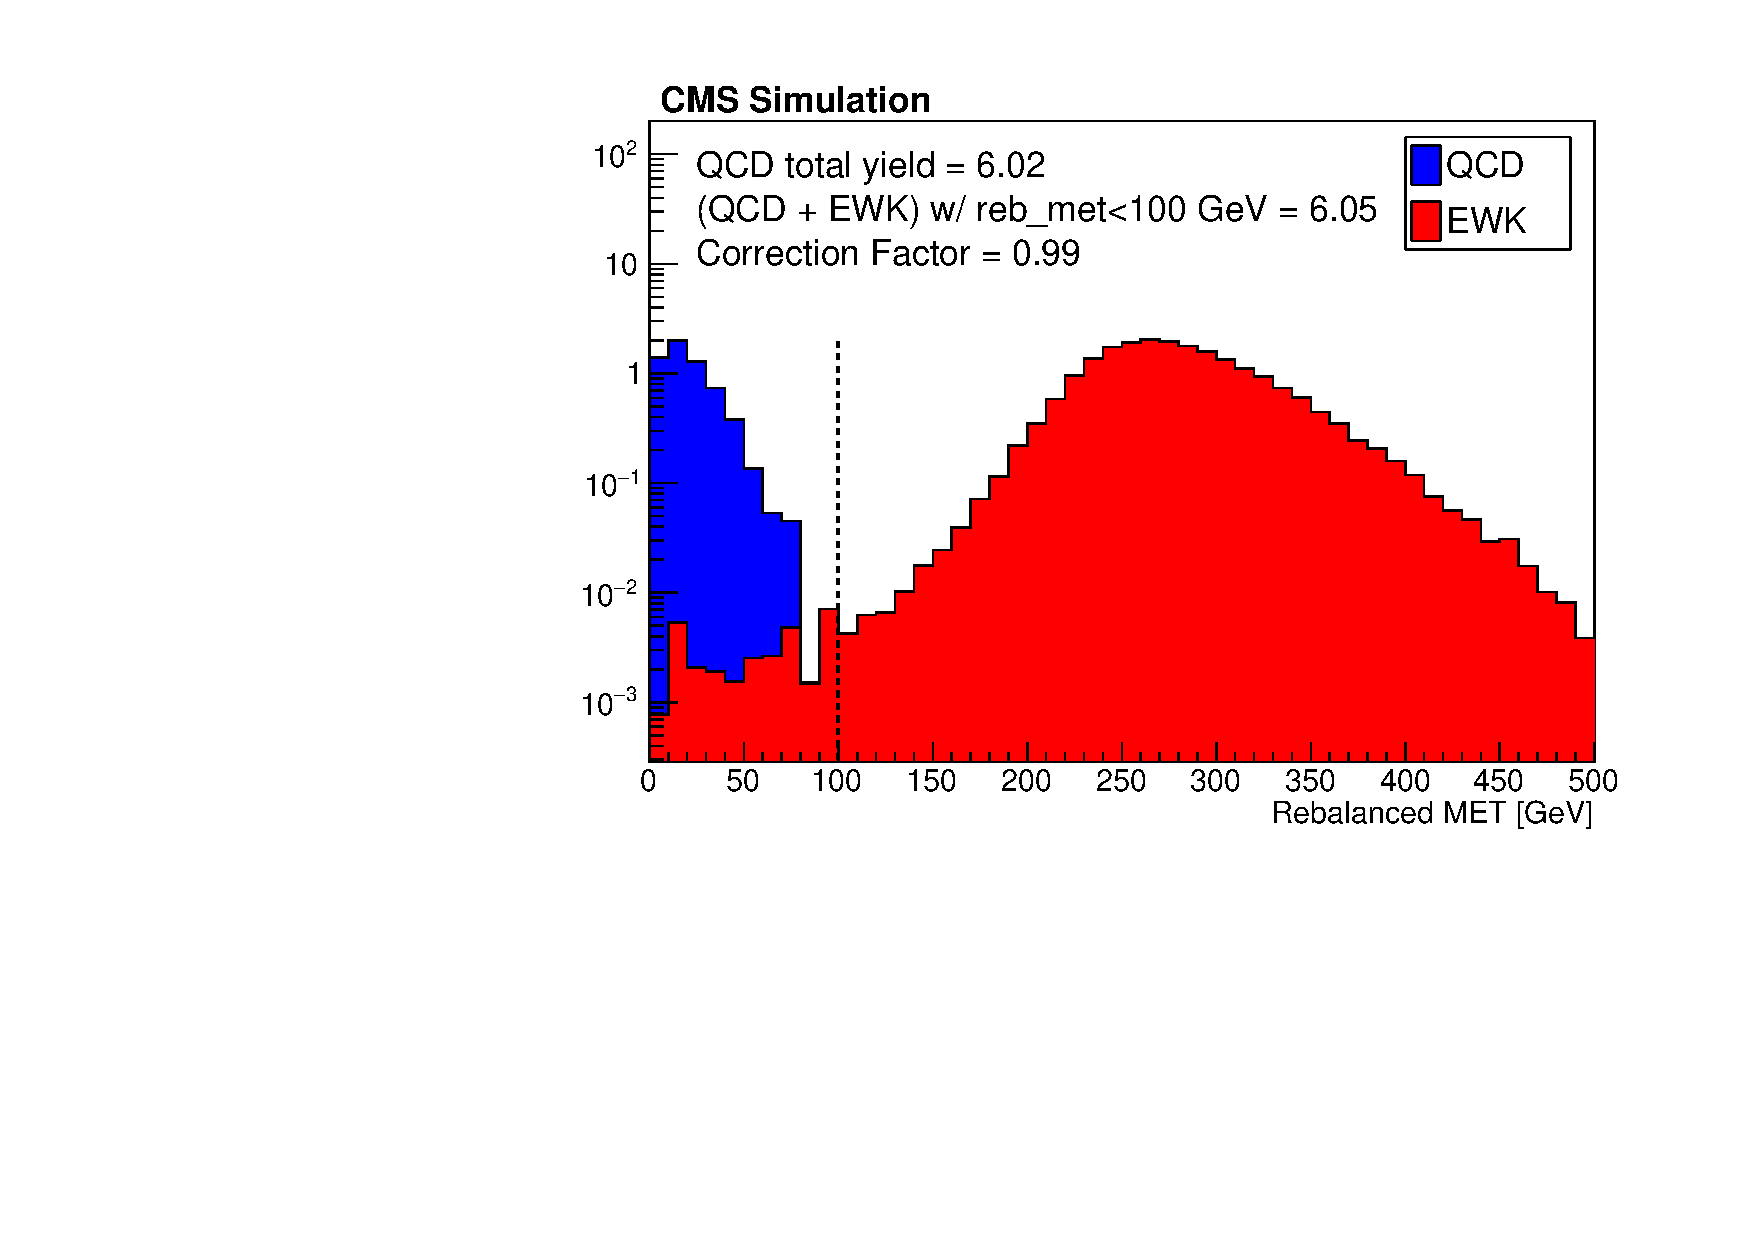
\includegraphics[width=0.45\textwidth]{figs/qcd/rs_mc/ewk/ewk_VL.pdf}
    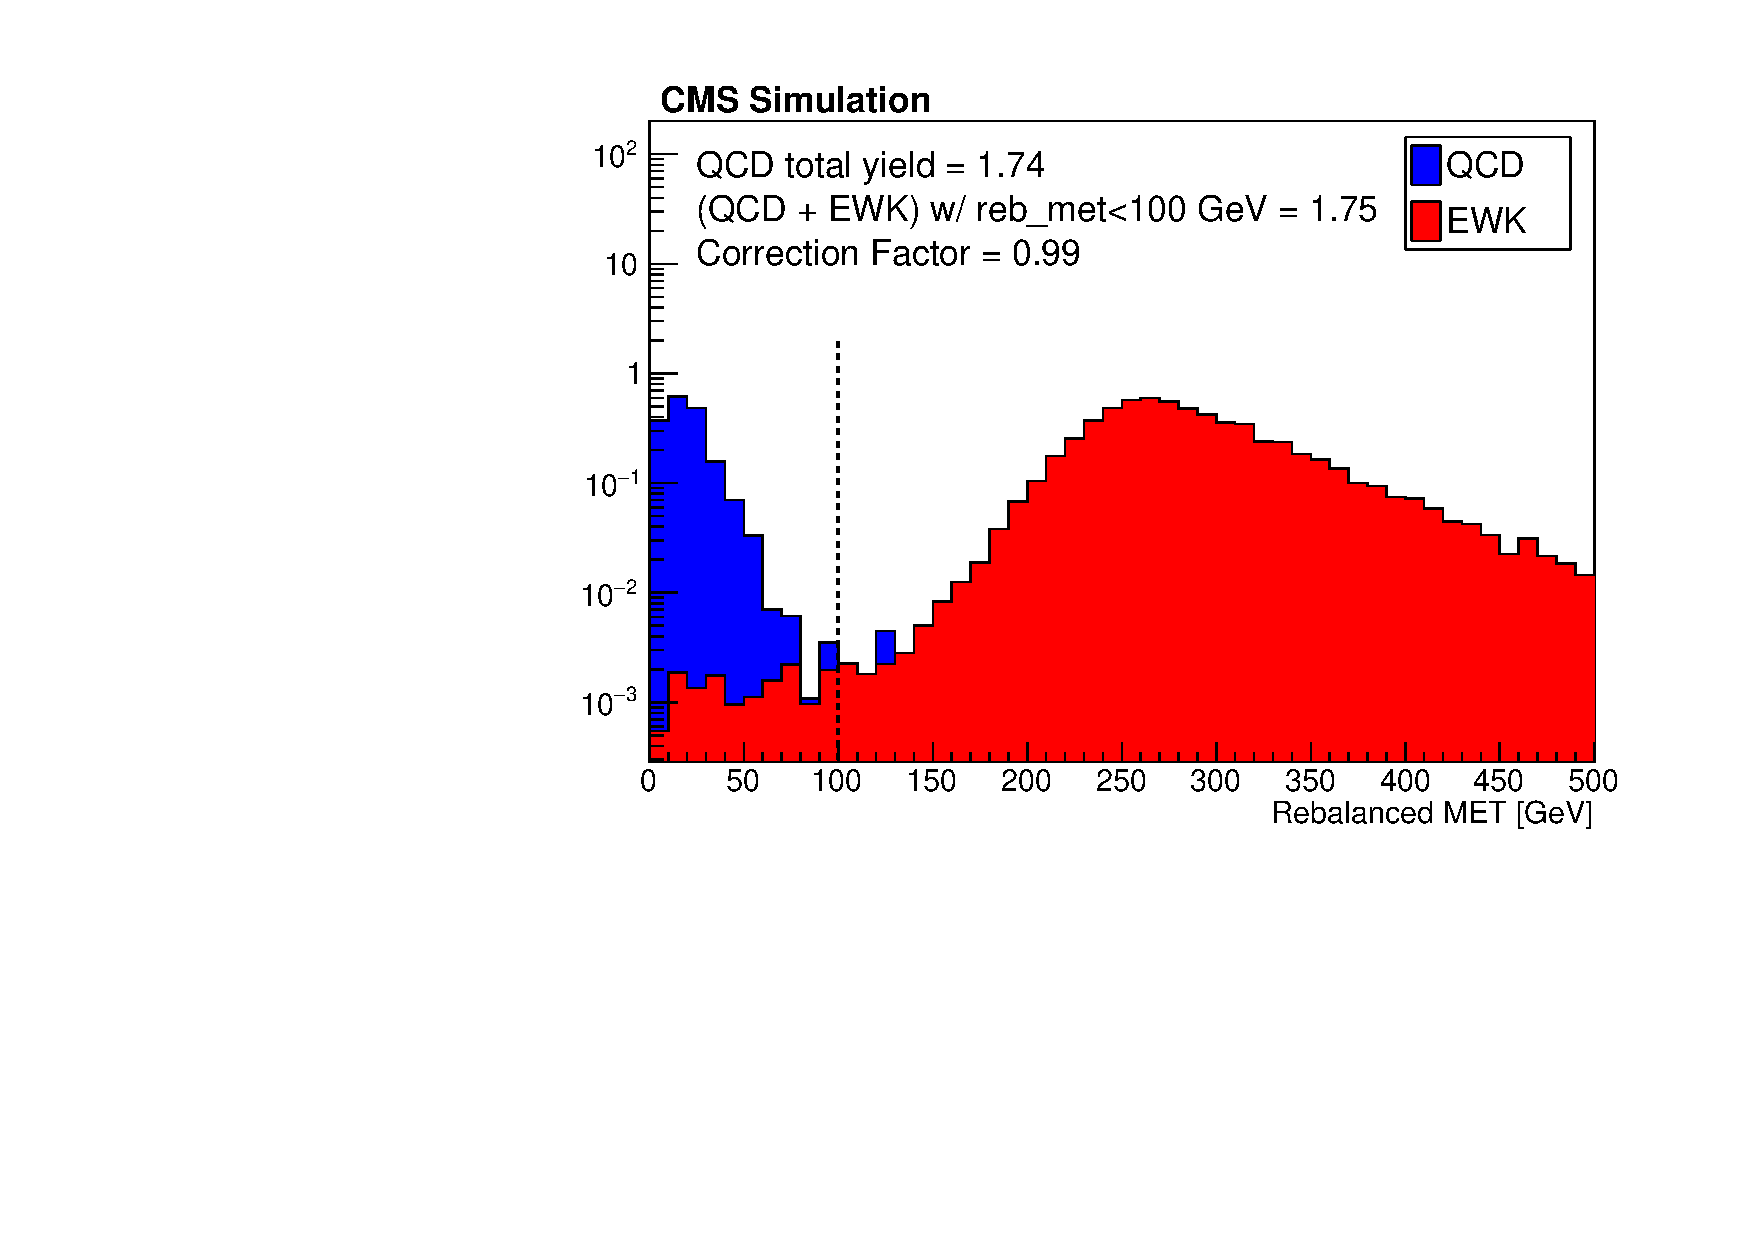
\includegraphics[width=0.45\textwidth]{figs/qcd/rs_mc/ewk/ewk_L.pdf}
    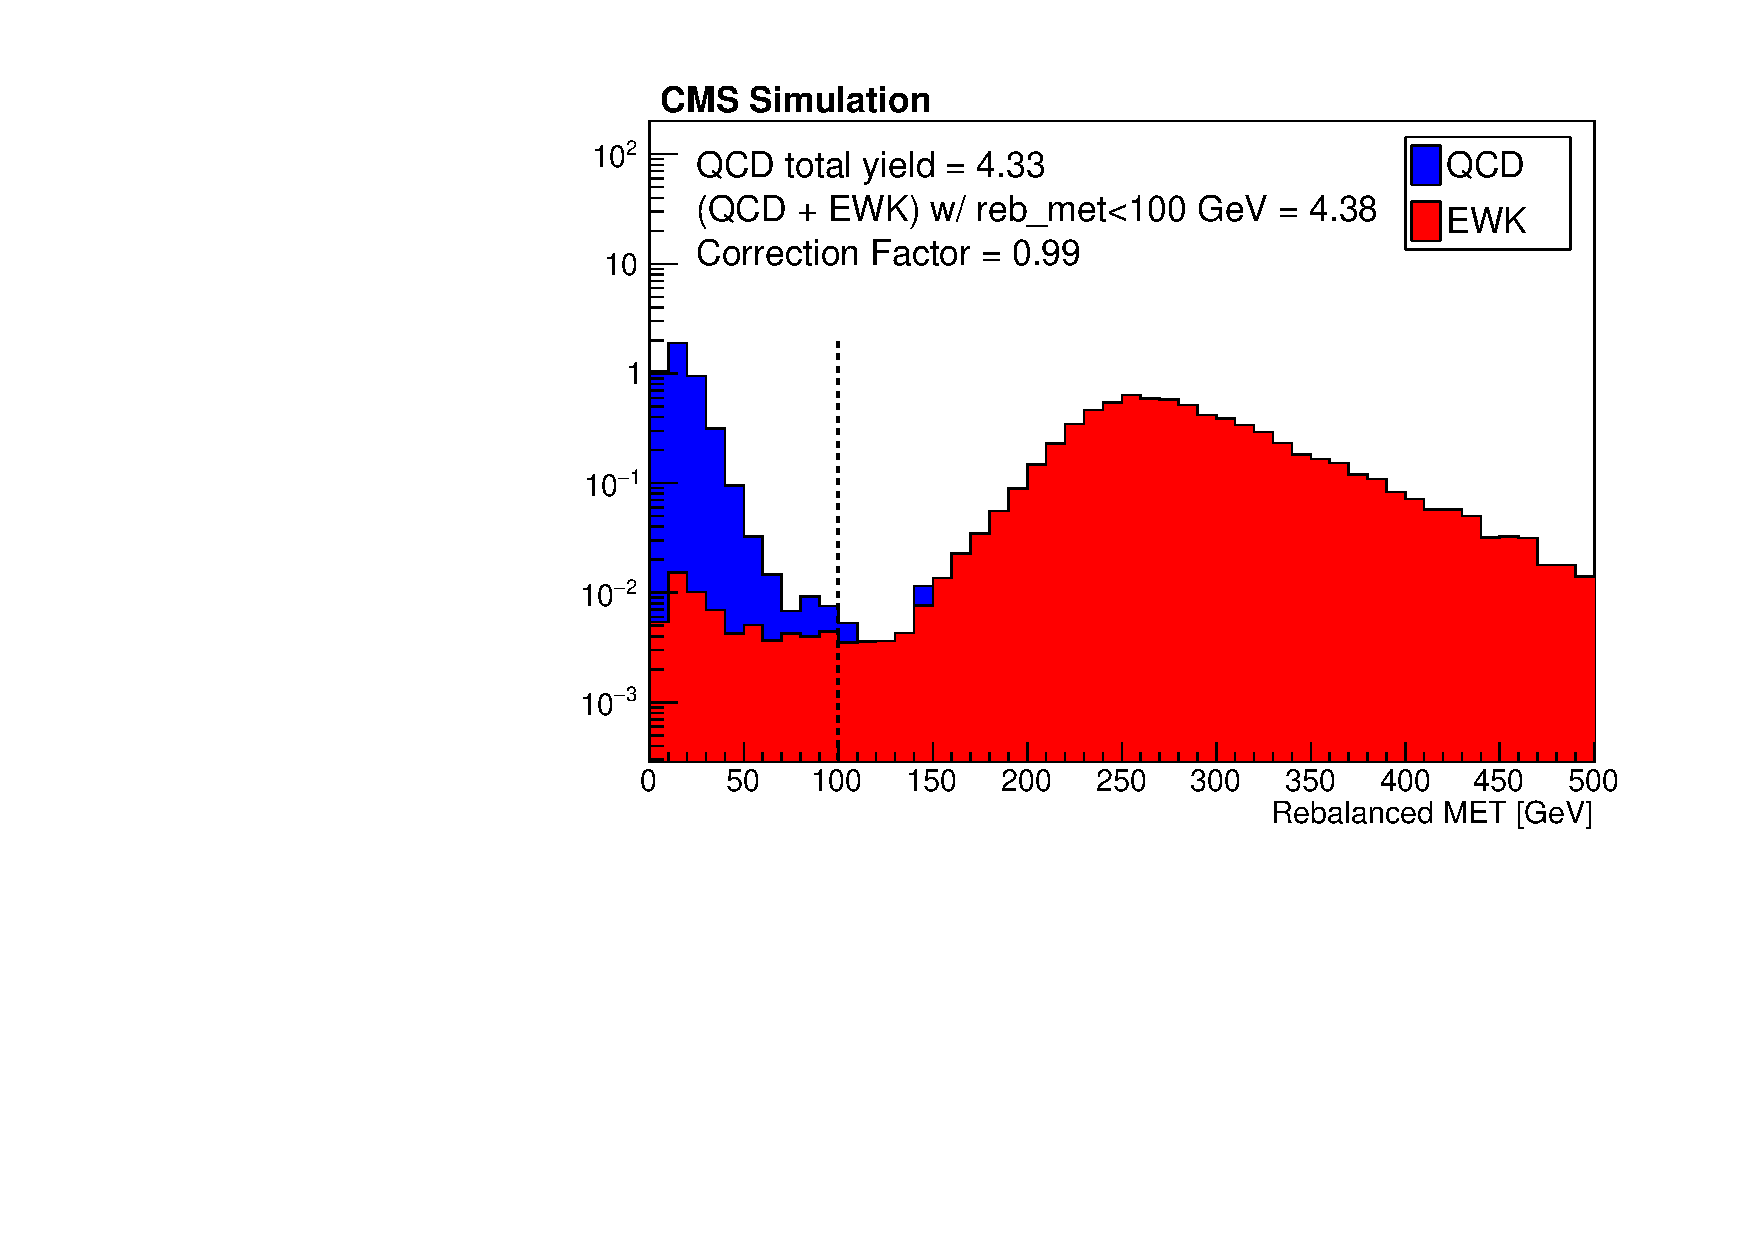
\includegraphics[width=0.45\textwidth]{figs/qcd/rs_mc/ewk/ewk_M.pdf}
    \caption{Rebalanced \ptmiss distribution for QCD and electroweak smeared events in the very low, low, and medium \Ht regions after the baseline selection.
            }
    \label{Fig:rs_ewk_low_med}
  \end{center}
\end{figure}

\begin{figure}[htbp]
  \begin{center}
    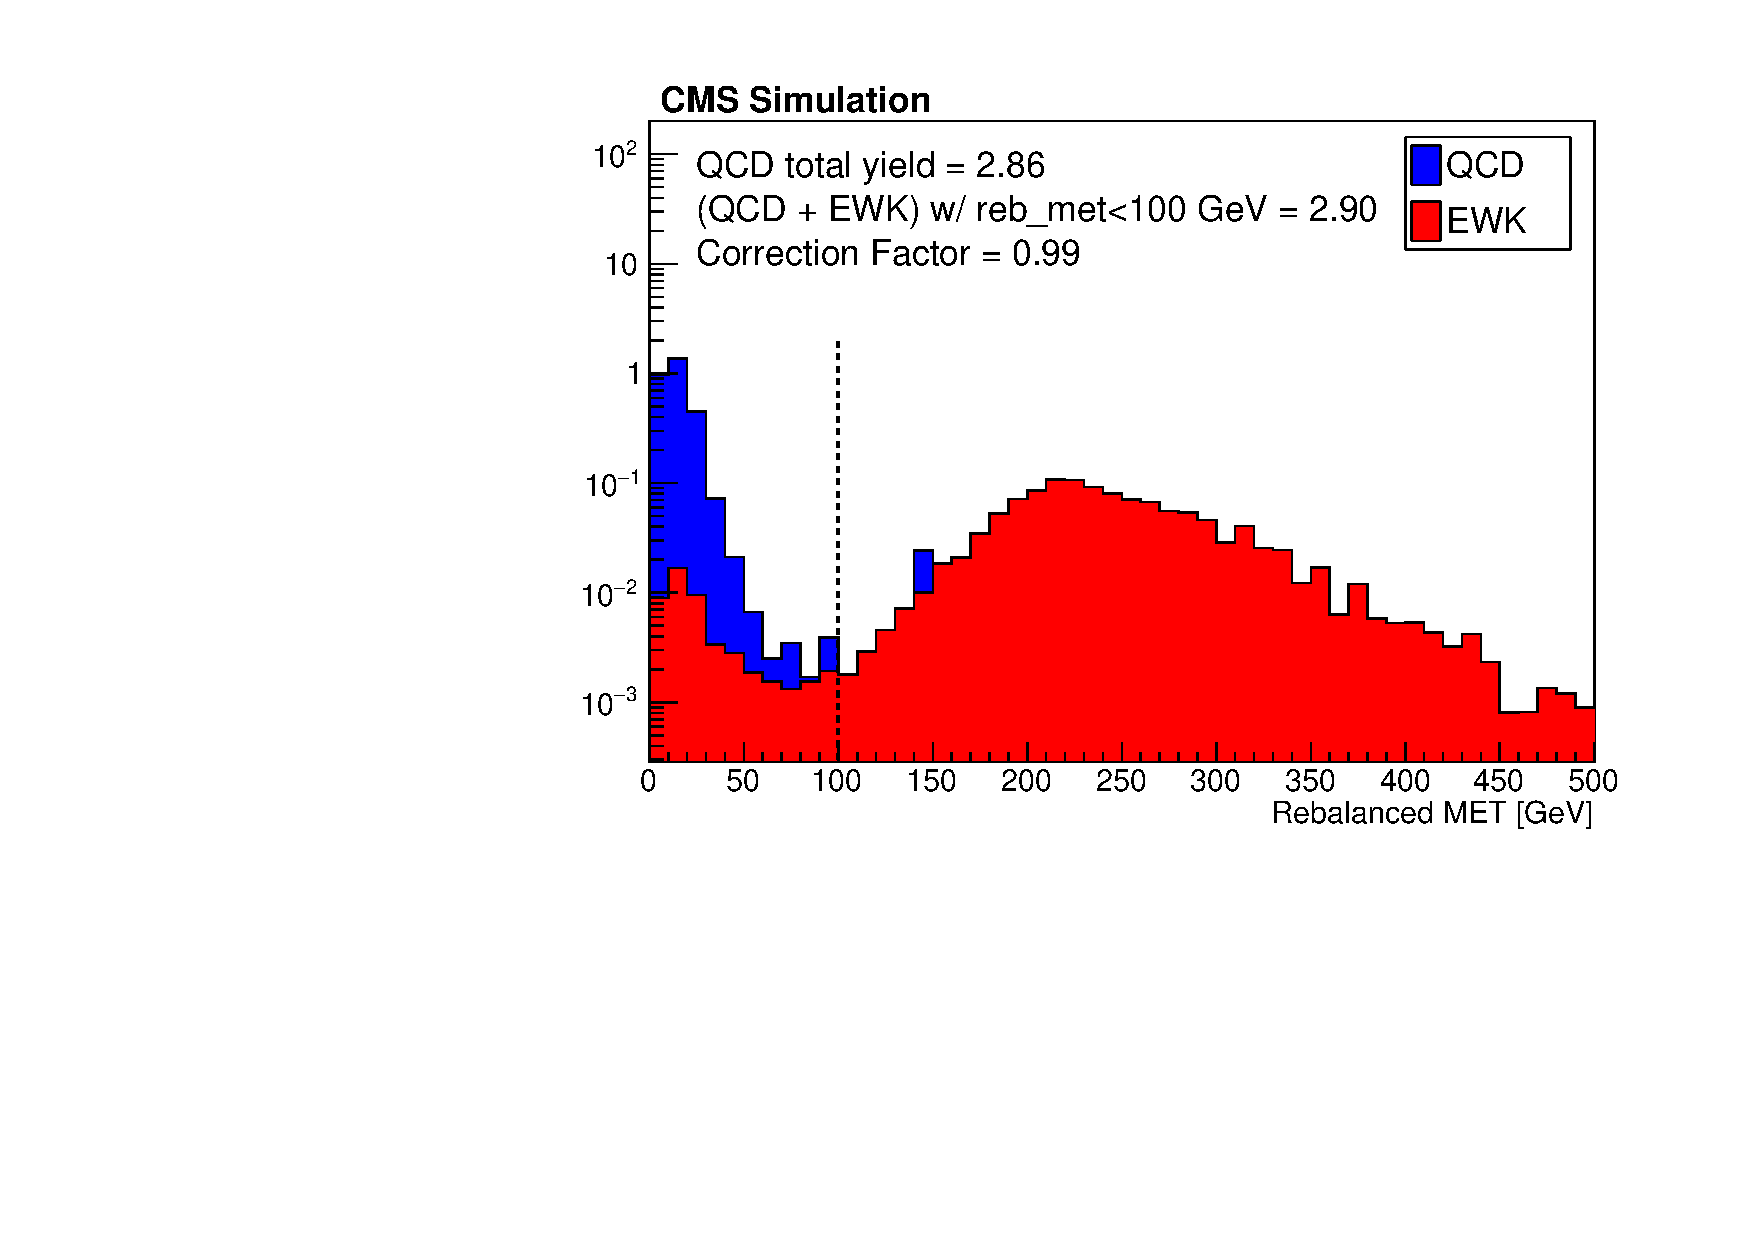
\includegraphics[width=0.45\textwidth]{figs/qcd/rs_mc/ewk/ewk_H.pdf}
    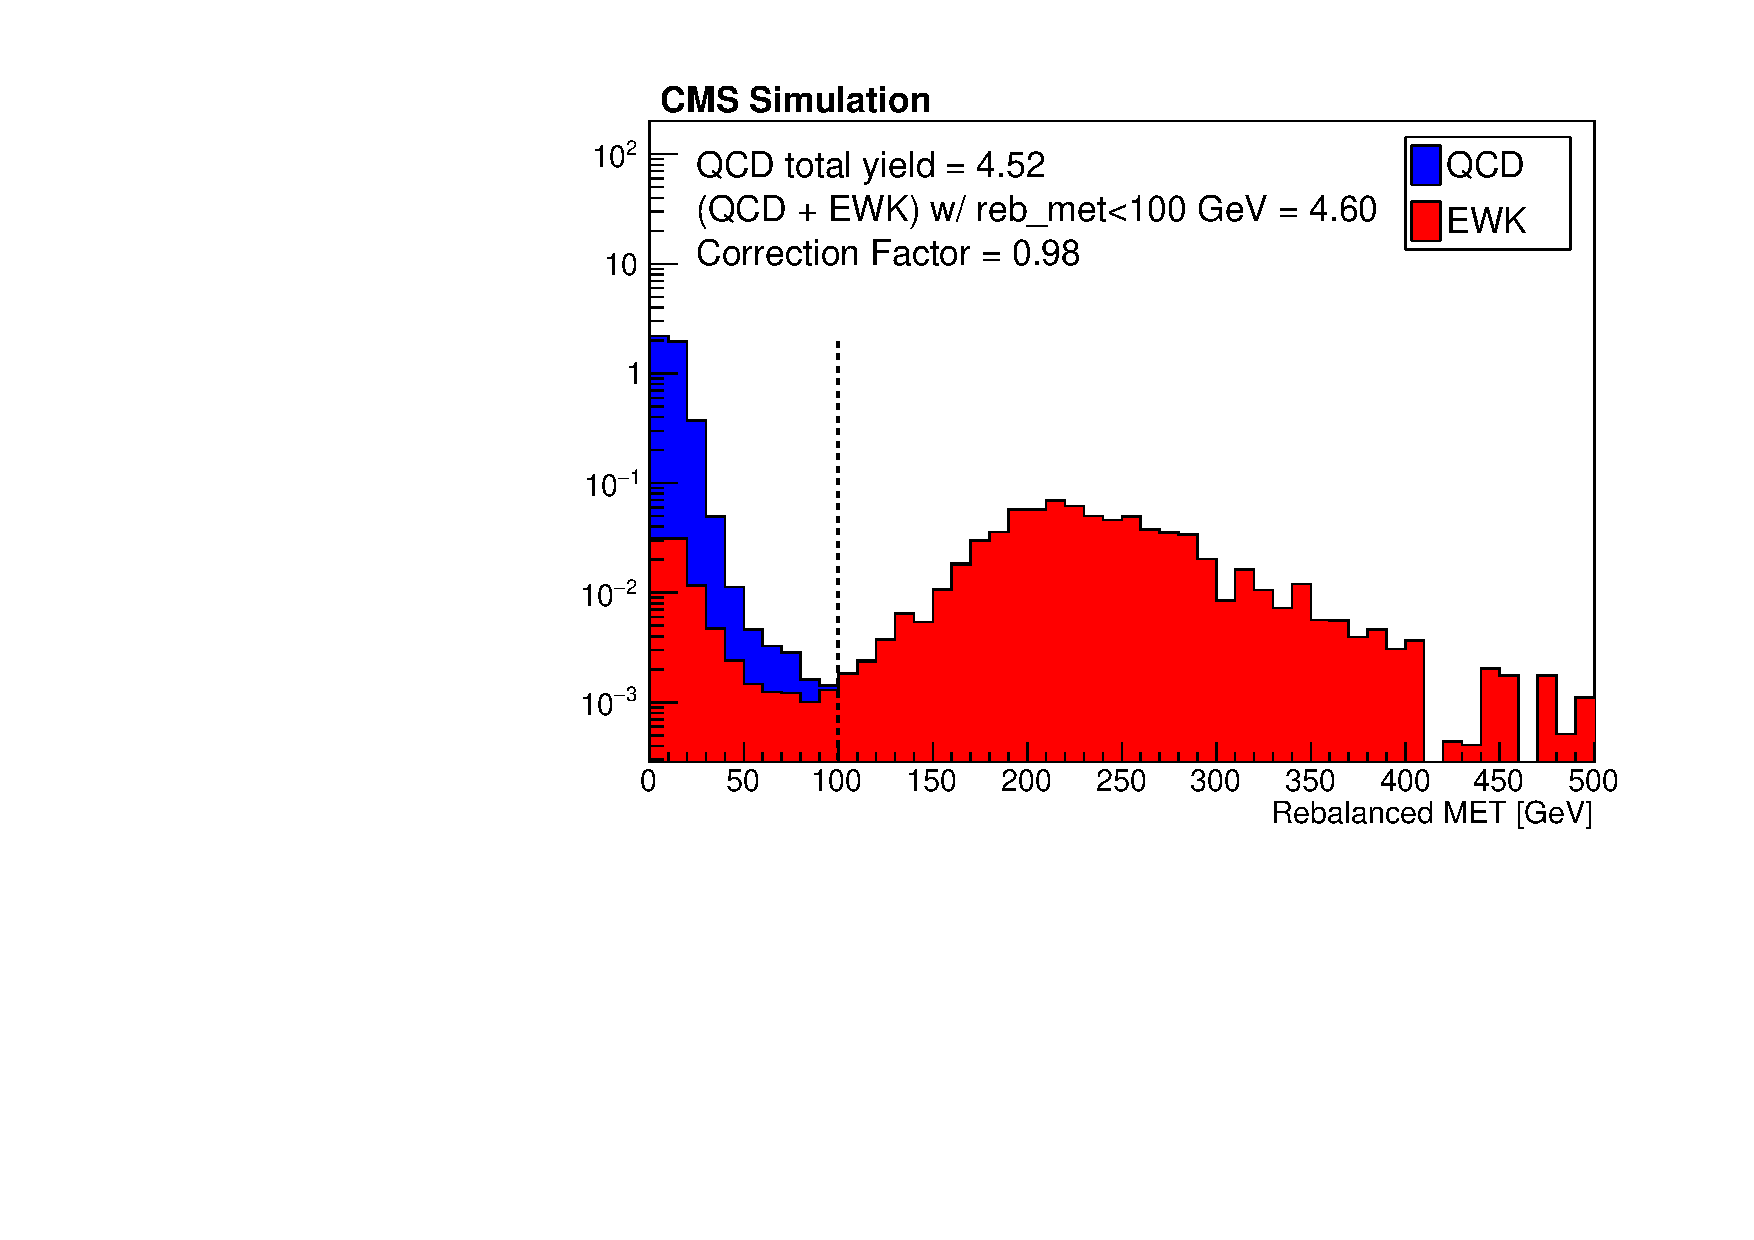
\includegraphics[width=0.45\textwidth]{figs/qcd/rs_mc/ewk/ewk_UH.pdf}
    \caption{Rebalanced \ptmiss distribution for QCD and electroweak smeared events in the high and extreme \Ht regions after the baseline selection.
            }
    \label{Fig:rs_ewk_high_ext}
  \end{center}
\end{figure}

\clearpage
\begin{table}[h]
\caption{Derivation of scale factors to correct for loss of QCD events due to the rebalanced $\ptmiss < 100$\GeV requirement.
The scale factor is found to be 1.00 in all \Ht regions.
\label{tab:rs_table_rebmet_sf}}
\centering
\begin{tabular}{lccccc}
%\hline
\hline
 & Very Low \Ht & Low \Ht & Med \Ht & High \Ht & Ext \Ht \\
\hline
%\hline
QCD total yield & 6.02 & 1.74 & 4.33 & 2.86 & 4.52 \\
%\hline
QCD + EWK, & \multirow{2}{*}{6.05} & \multirow{2}{*}{1.75} & \multirow{2}{*}{4.38} & \multirow{2}{*}{2.90} & \multirow{2}{*}{4.60} \\
reb $\ptmiss < 100$\GeV & & & & & \\
\hline
Correction Factor & 0.99 & 0.99 & 0.99 & 0.99 & 0.98 \\
\hline
\end{tabular}
\end{table}

\section{Performance in data control regions}

In order to gauge the performance of the \rs method in data we define three control regions that are orthogonal to the search regions and enriched in QCD events.
The first control region is obtained from the baseline selection by inverting the $\dpmin$ cut, requiring $\dpmin < 0.3$. The second control region is the $\mttwo$
sideband $100< \mttwo <$ 200\GeV. The third control region is defined by both inverting the $\dpmin$ selection and selecting the $\mttwo$ sideband. Figures
~\ref{Fig:rs_crRSInvertDPhiInclusiveHT1200toInf}--\ref{Fig:rs_crRSDPhiMT2InclusiveHT450to1200} show several kinematic distributions in the control regions for
$450 <\Ht<$ 1200\GeV and $\Ht > 1200$\GeV separately. Non-QCD background contributions in these control regions are taken from Monte Carlo. Selecting just the $\mttwo$
sideband or just inverting \dpmin for $450<\Ht<$ 1200\GeV is not enough to make QCD a significant fraction of the total background in this \Ht region,
 so these plots are not shown.

\begin{figure}[!htbp]
  \begin{center}
    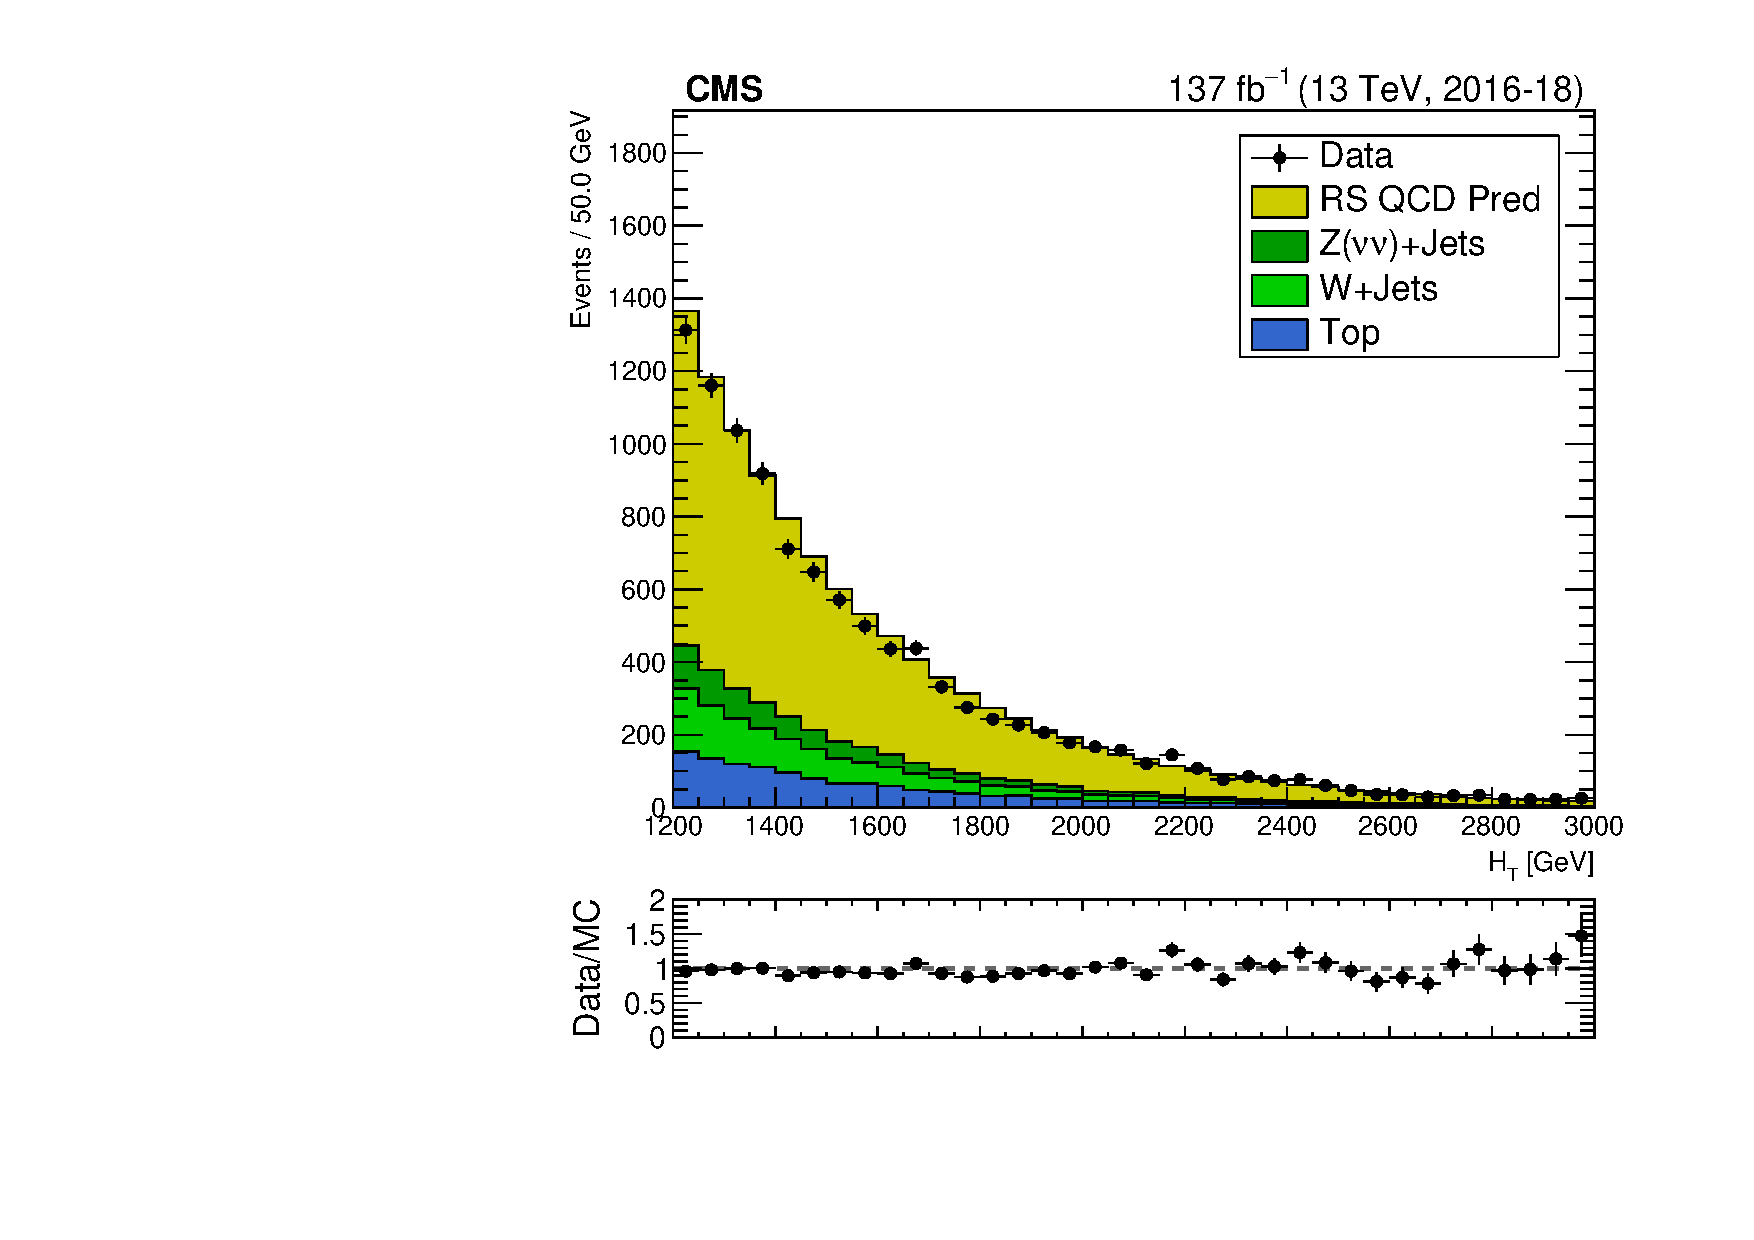
\includegraphics[width=0.46\textwidth]{figs/qcd/rs_data/c_crRSInvertDPhiInclusiveHT1200toInf_h_ht.pdf}
    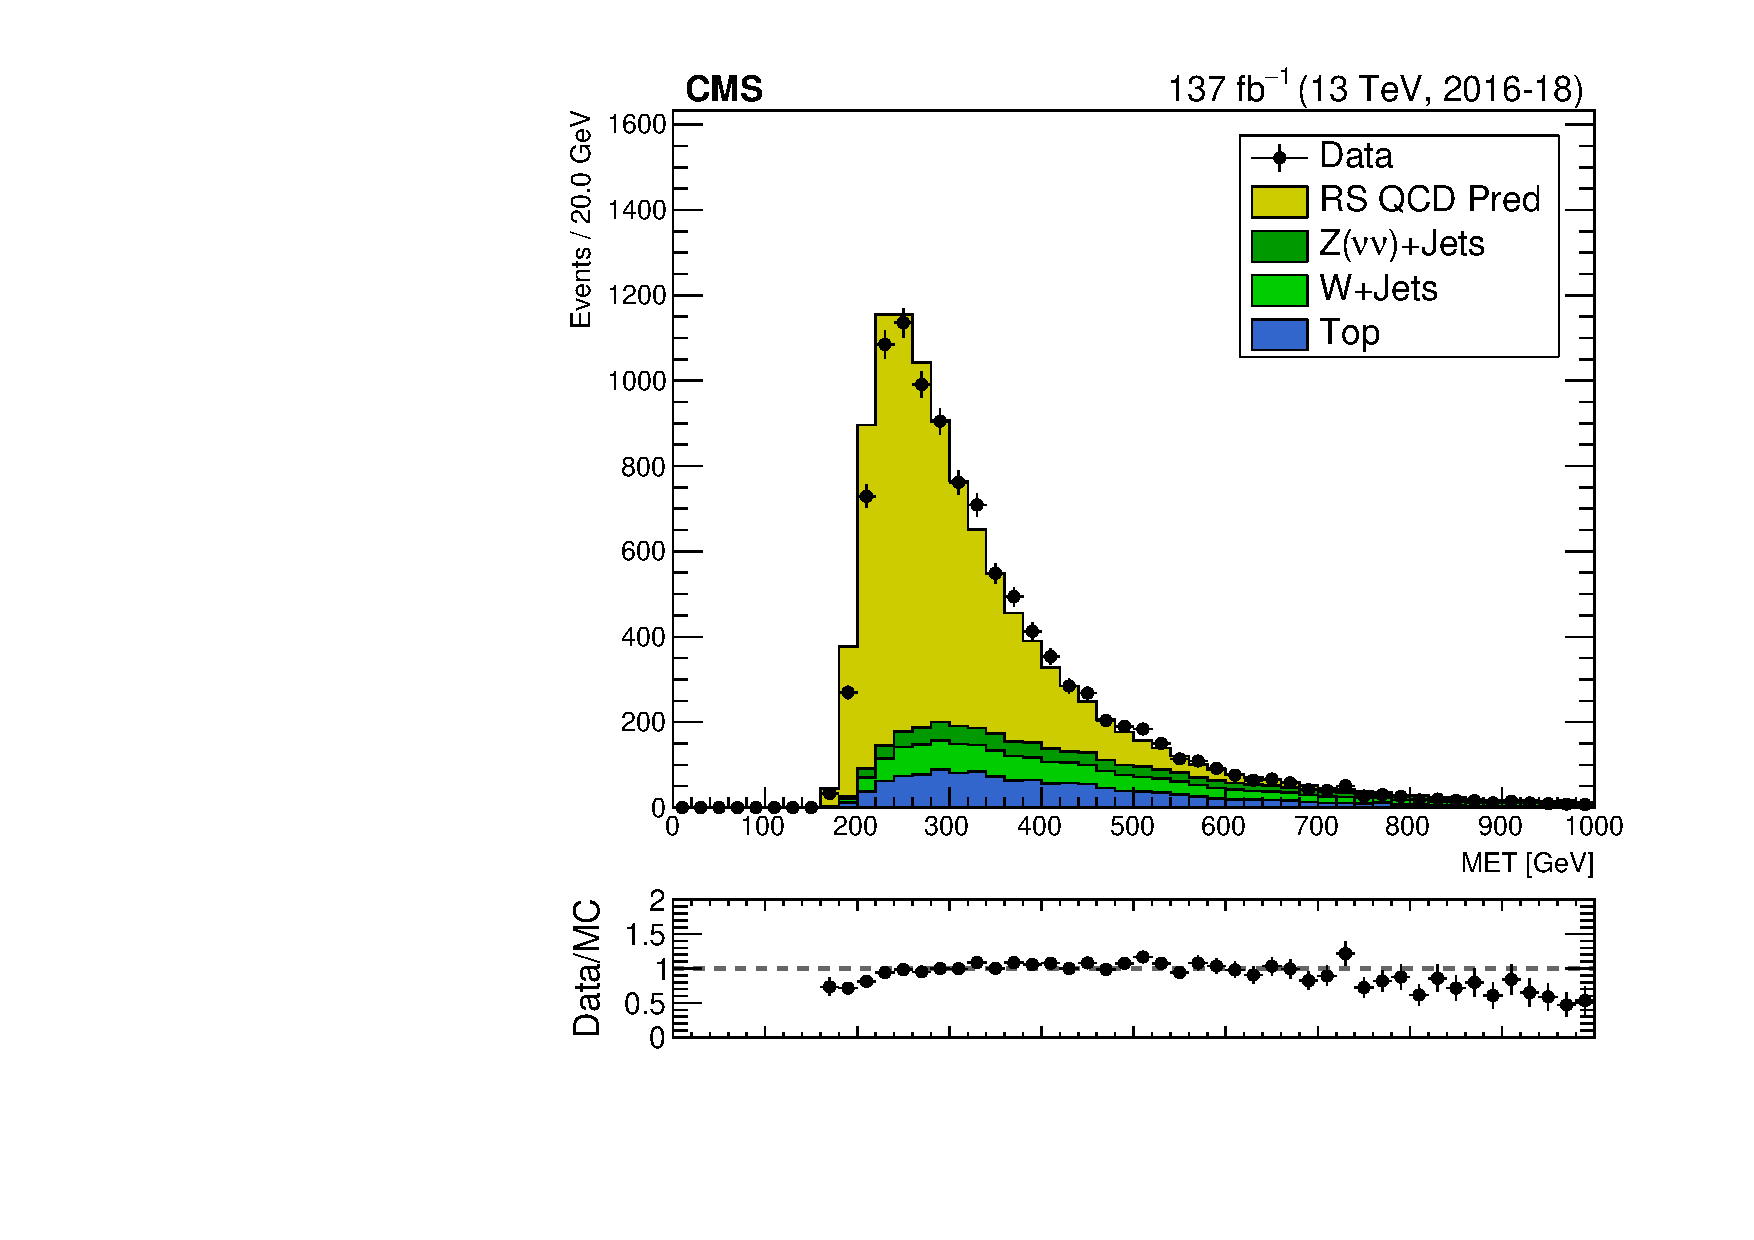
\includegraphics[width=0.46\textwidth]{figs/qcd/rs_data/c_crRSInvertDPhiInclusiveHT1200toInf_h_met.pdf}
    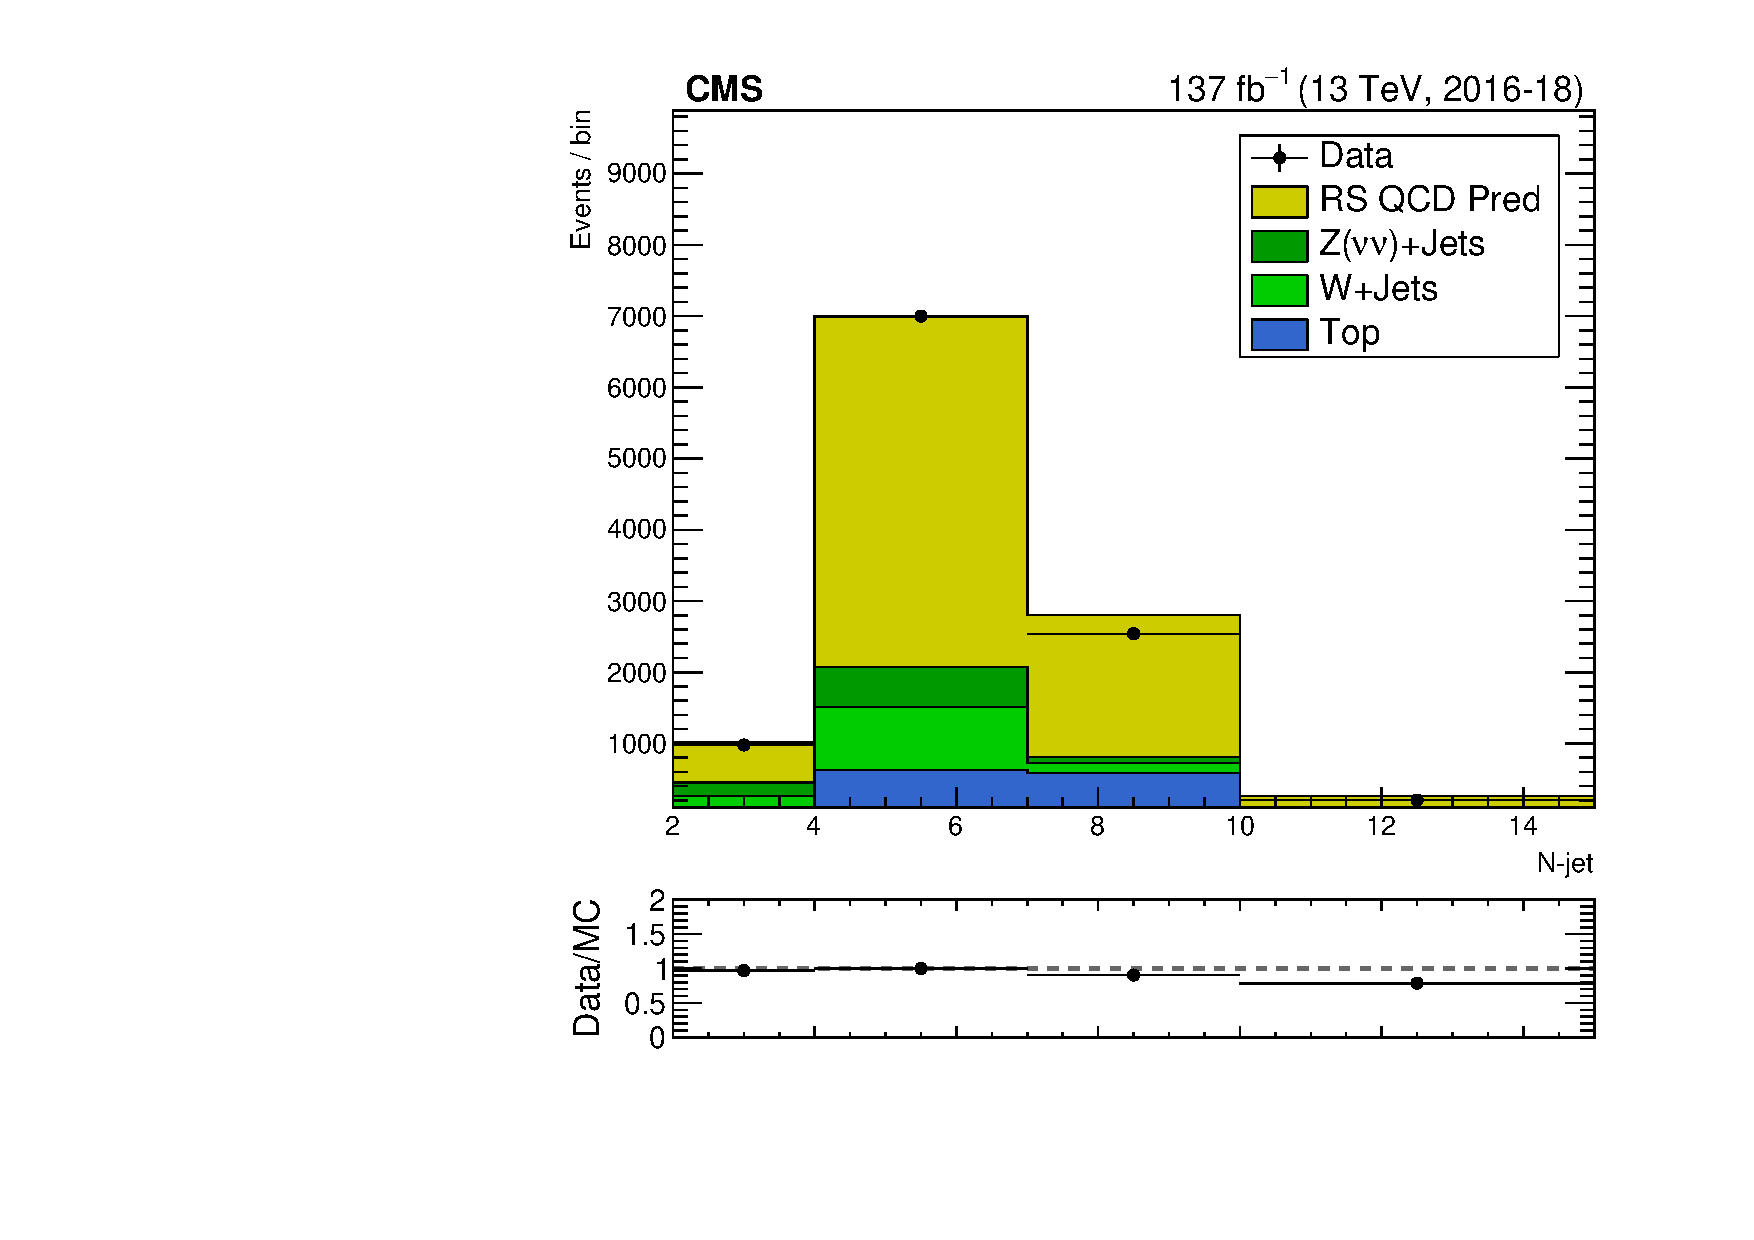
\includegraphics[width=0.46\textwidth]{figs/qcd/rs_data/c_crRSInvertDPhiInclusiveHT1200toInf_h_nJet30.pdf}
    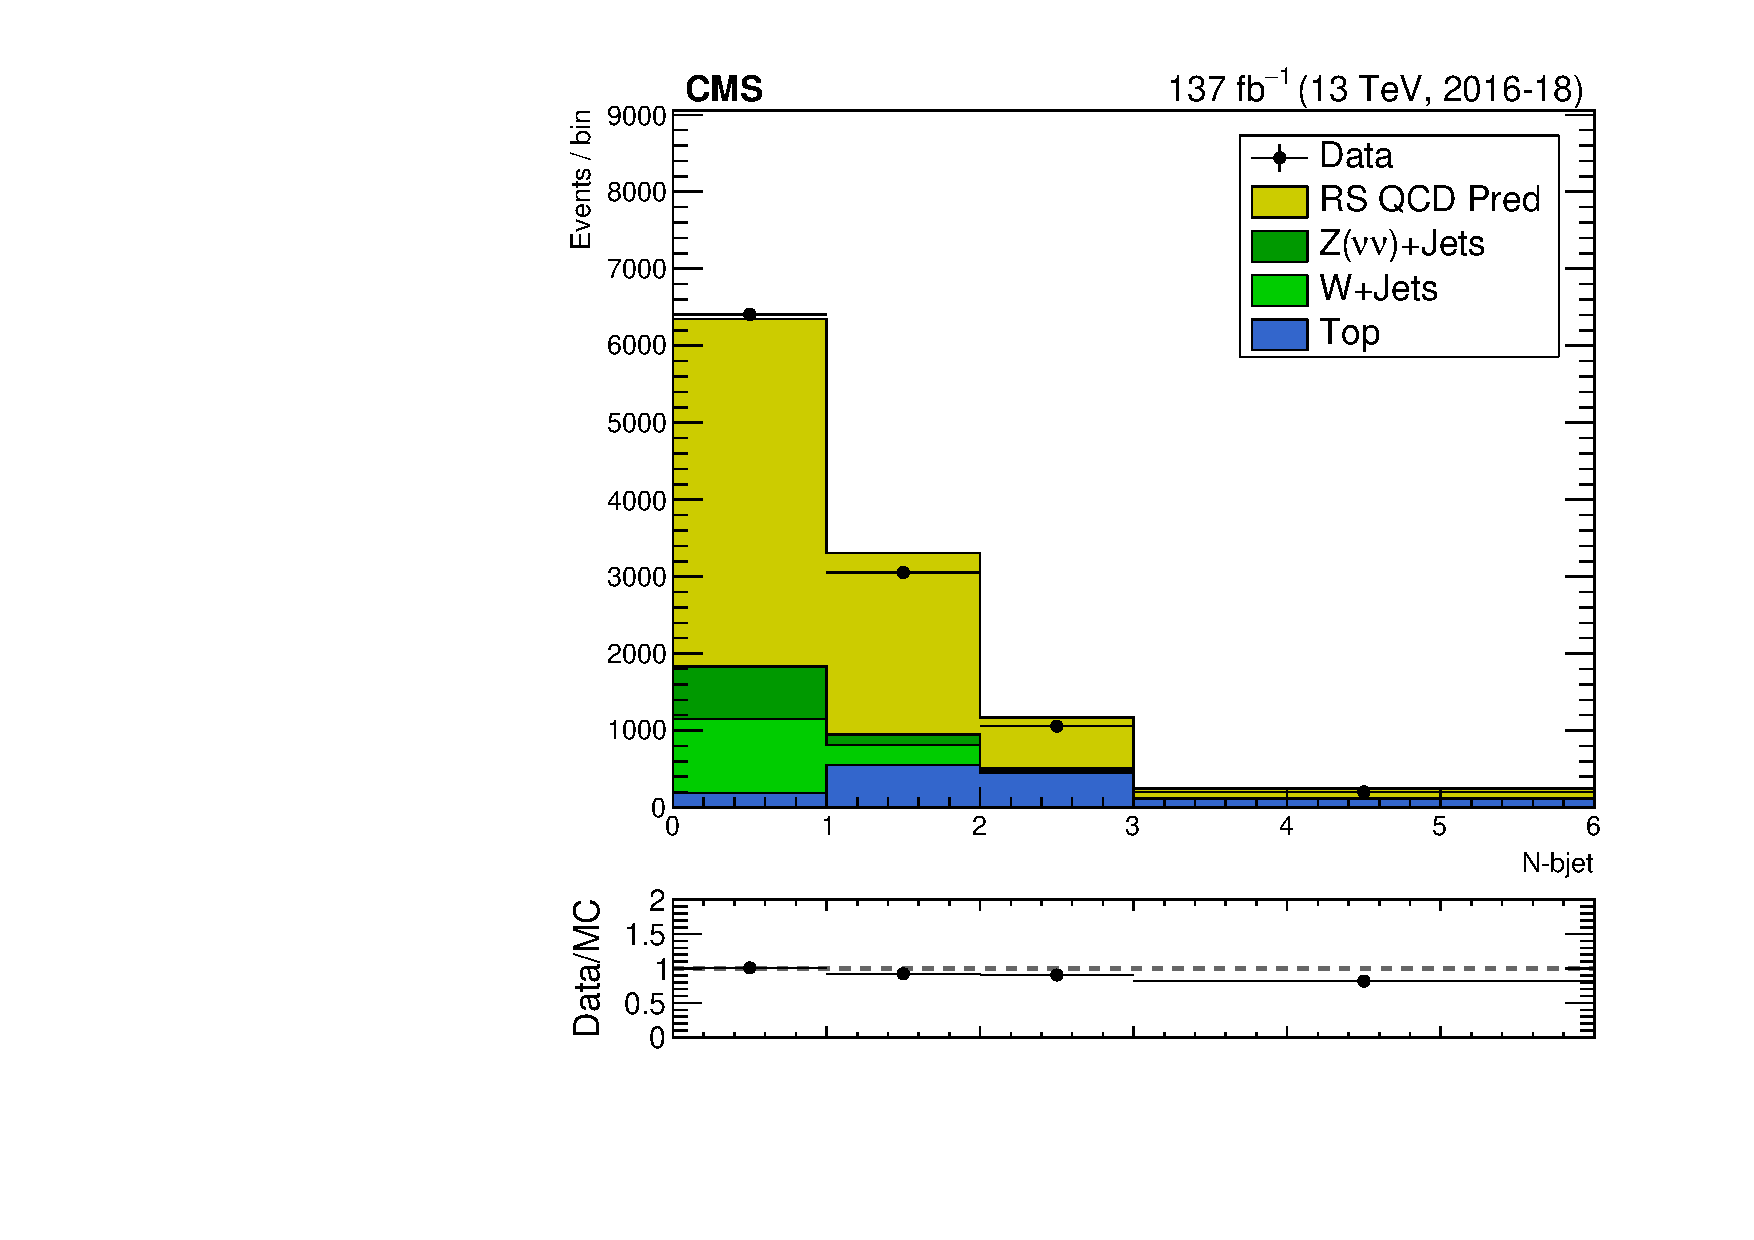
\includegraphics[width=0.46\textwidth]{figs/qcd/rs_data/c_crRSInvertDPhiInclusiveHT1200toInf_h_nBJet20.pdf}
    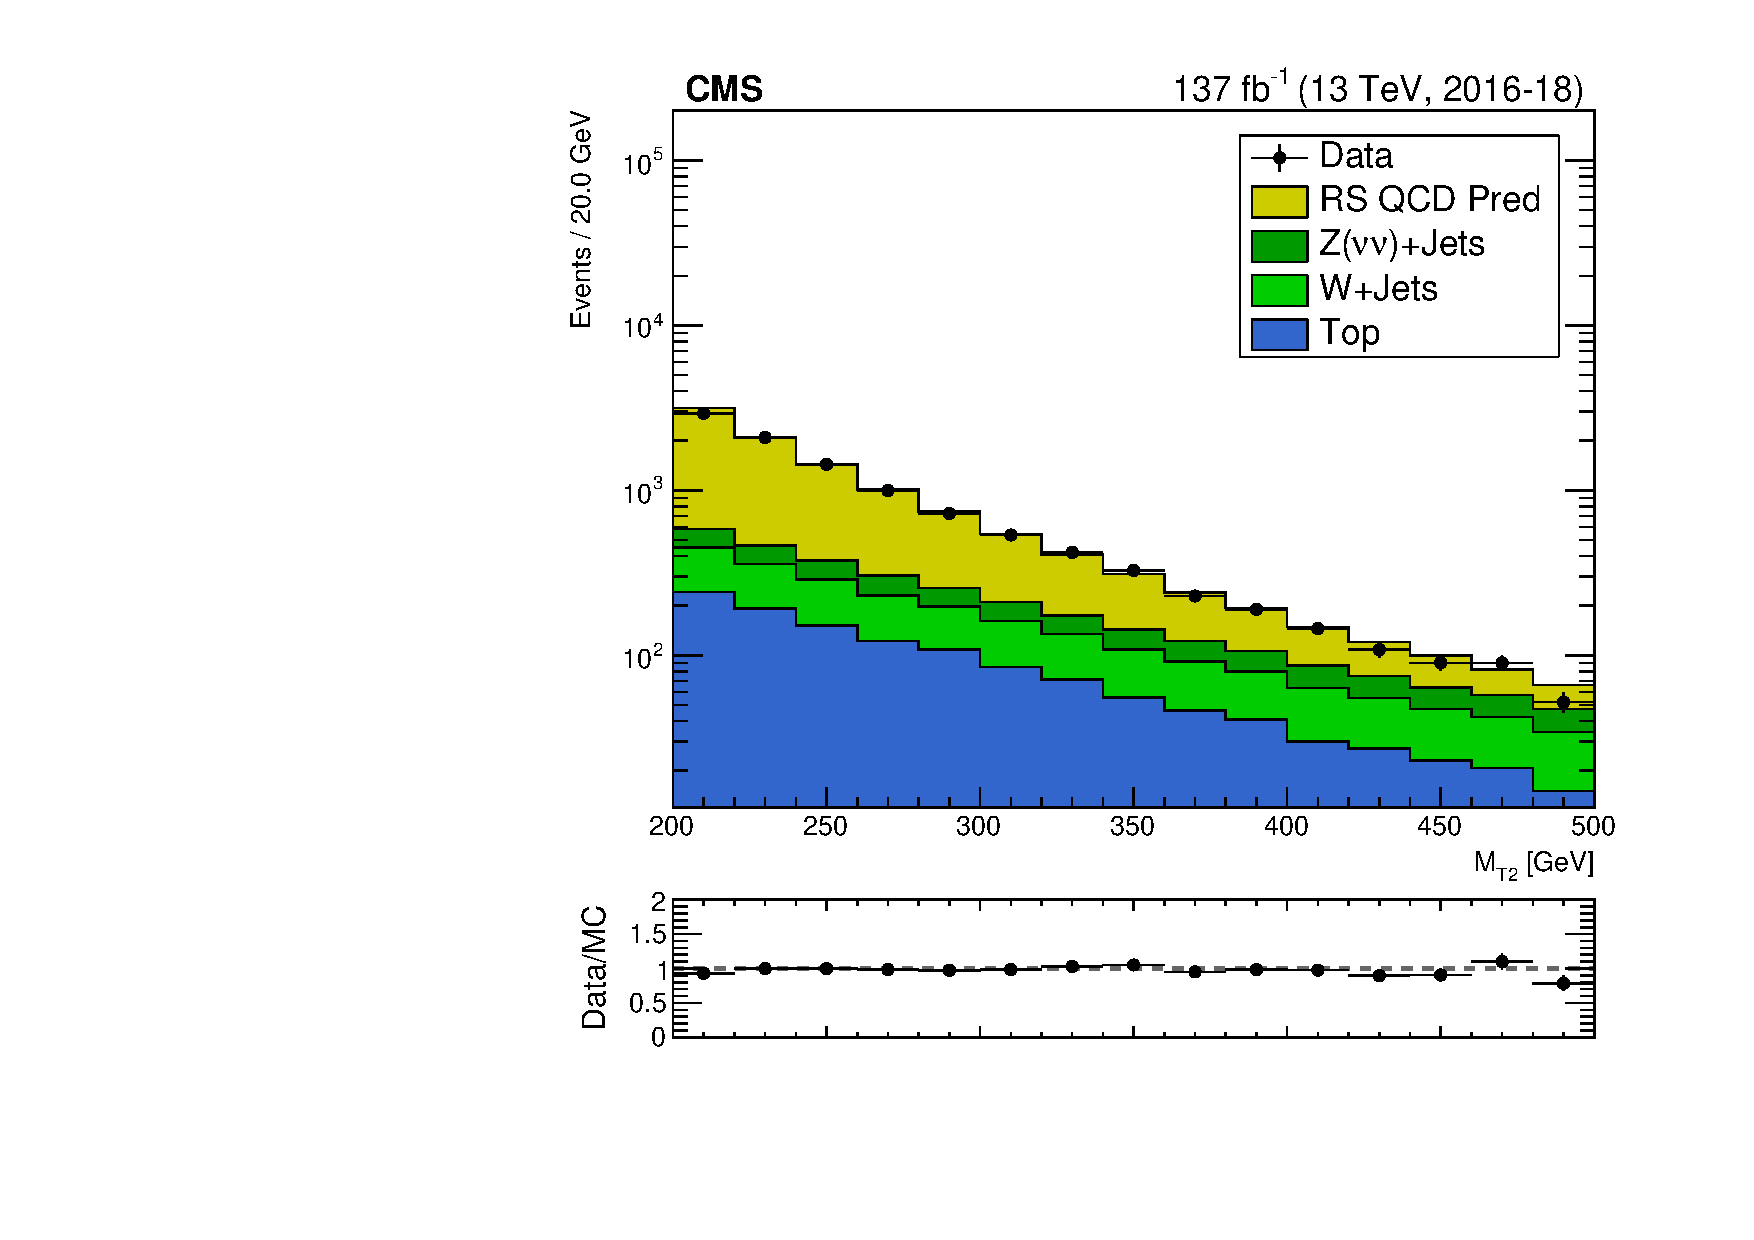
\includegraphics[width=0.46\textwidth]{figs/qcd/rs_data/c_crRSInvertDPhiInclusiveHT1200toInf_h_mt2.pdf}
    \caption{Comparison of kinematic distributions for data and background in the inverted $\dpmin$ control region for $\Ht > 1200$\GeV. The QCD background is from the
             rebalance and smear data-driven prediction. Non-QCD backgrounds are taken from Monte Carlo.
            }
    \label{Fig:rs_crRSInvertDPhiInclusiveHT1200toInf}
  \end{center}
\end{figure}

\begin{figure}[!htbp]
  \begin{center}
    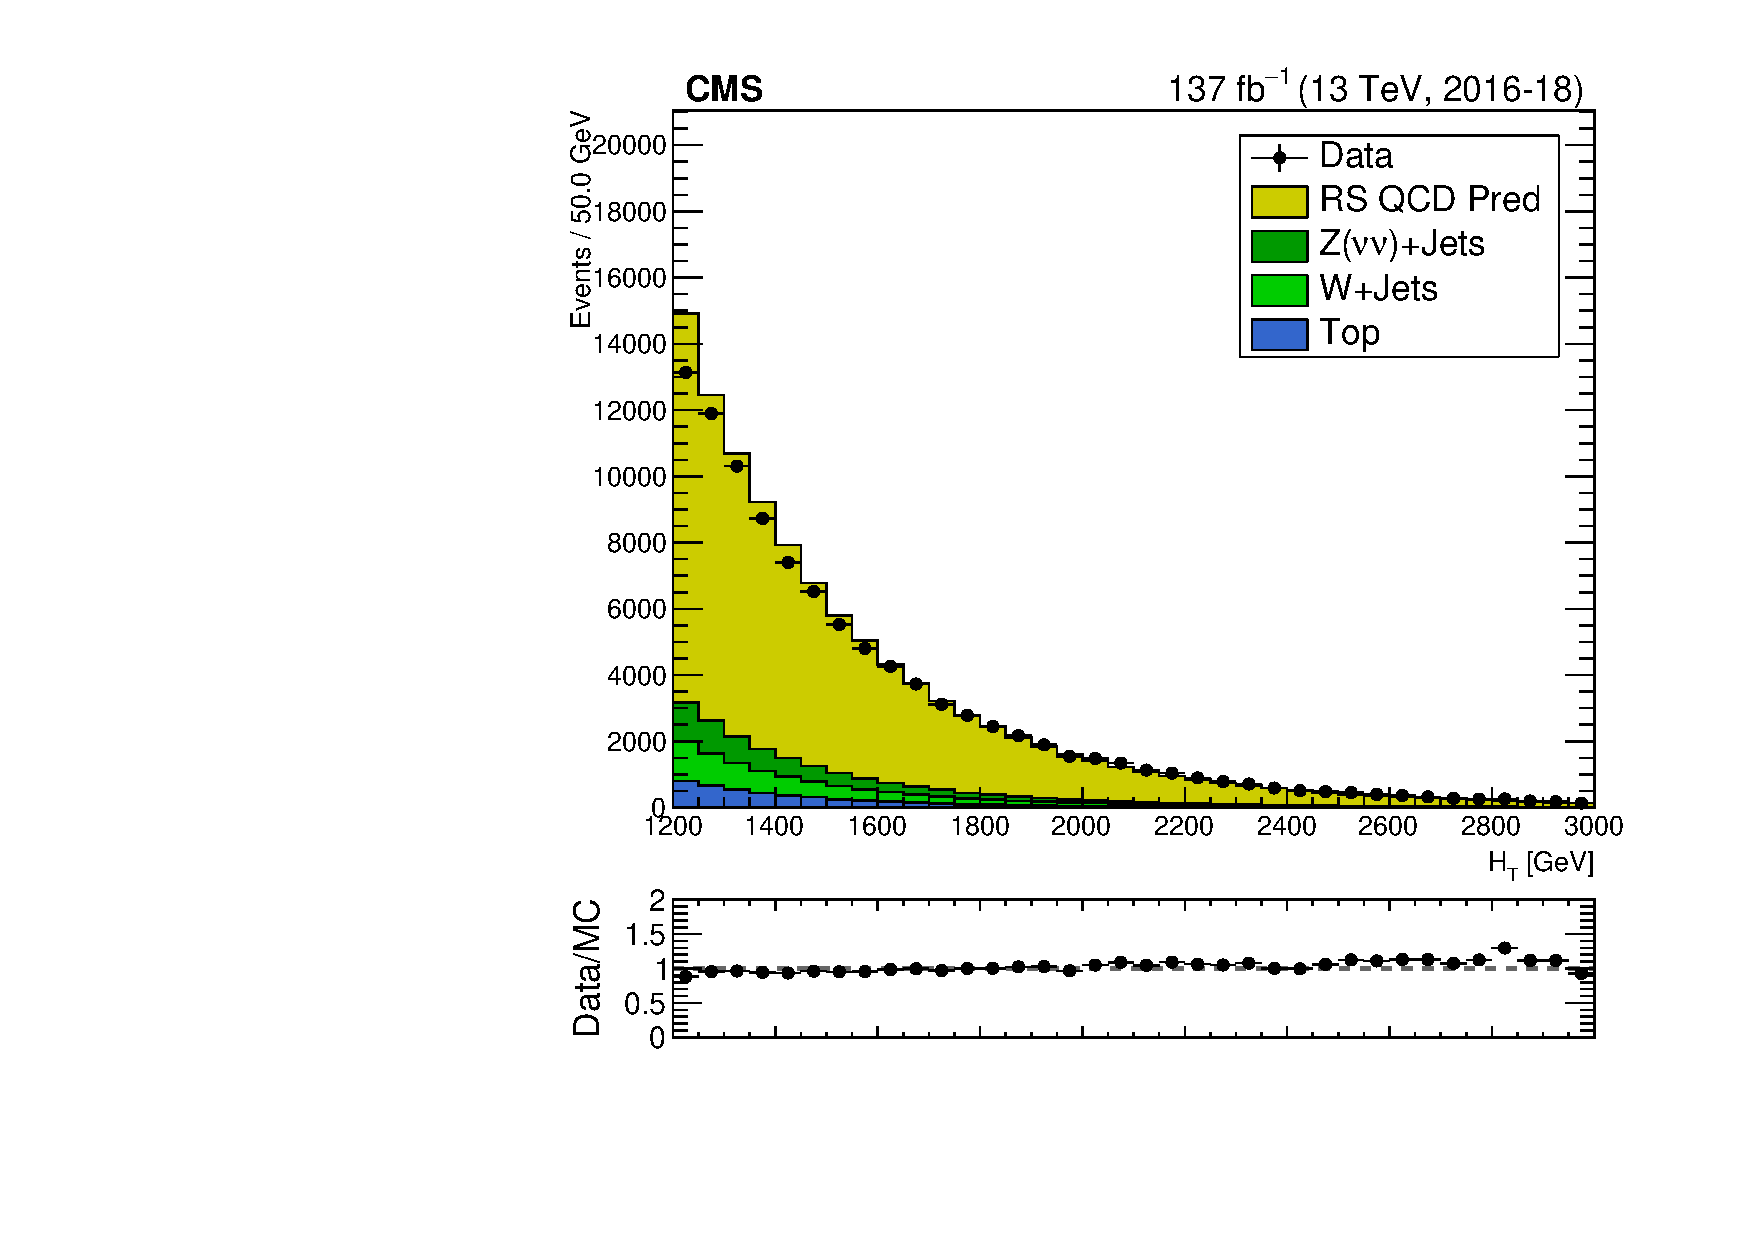
\includegraphics[width=0.46\textwidth]{figs/qcd/rs_data/c_crRSMT2SideBandInclusiveHT1200toInf_h_ht.pdf}
    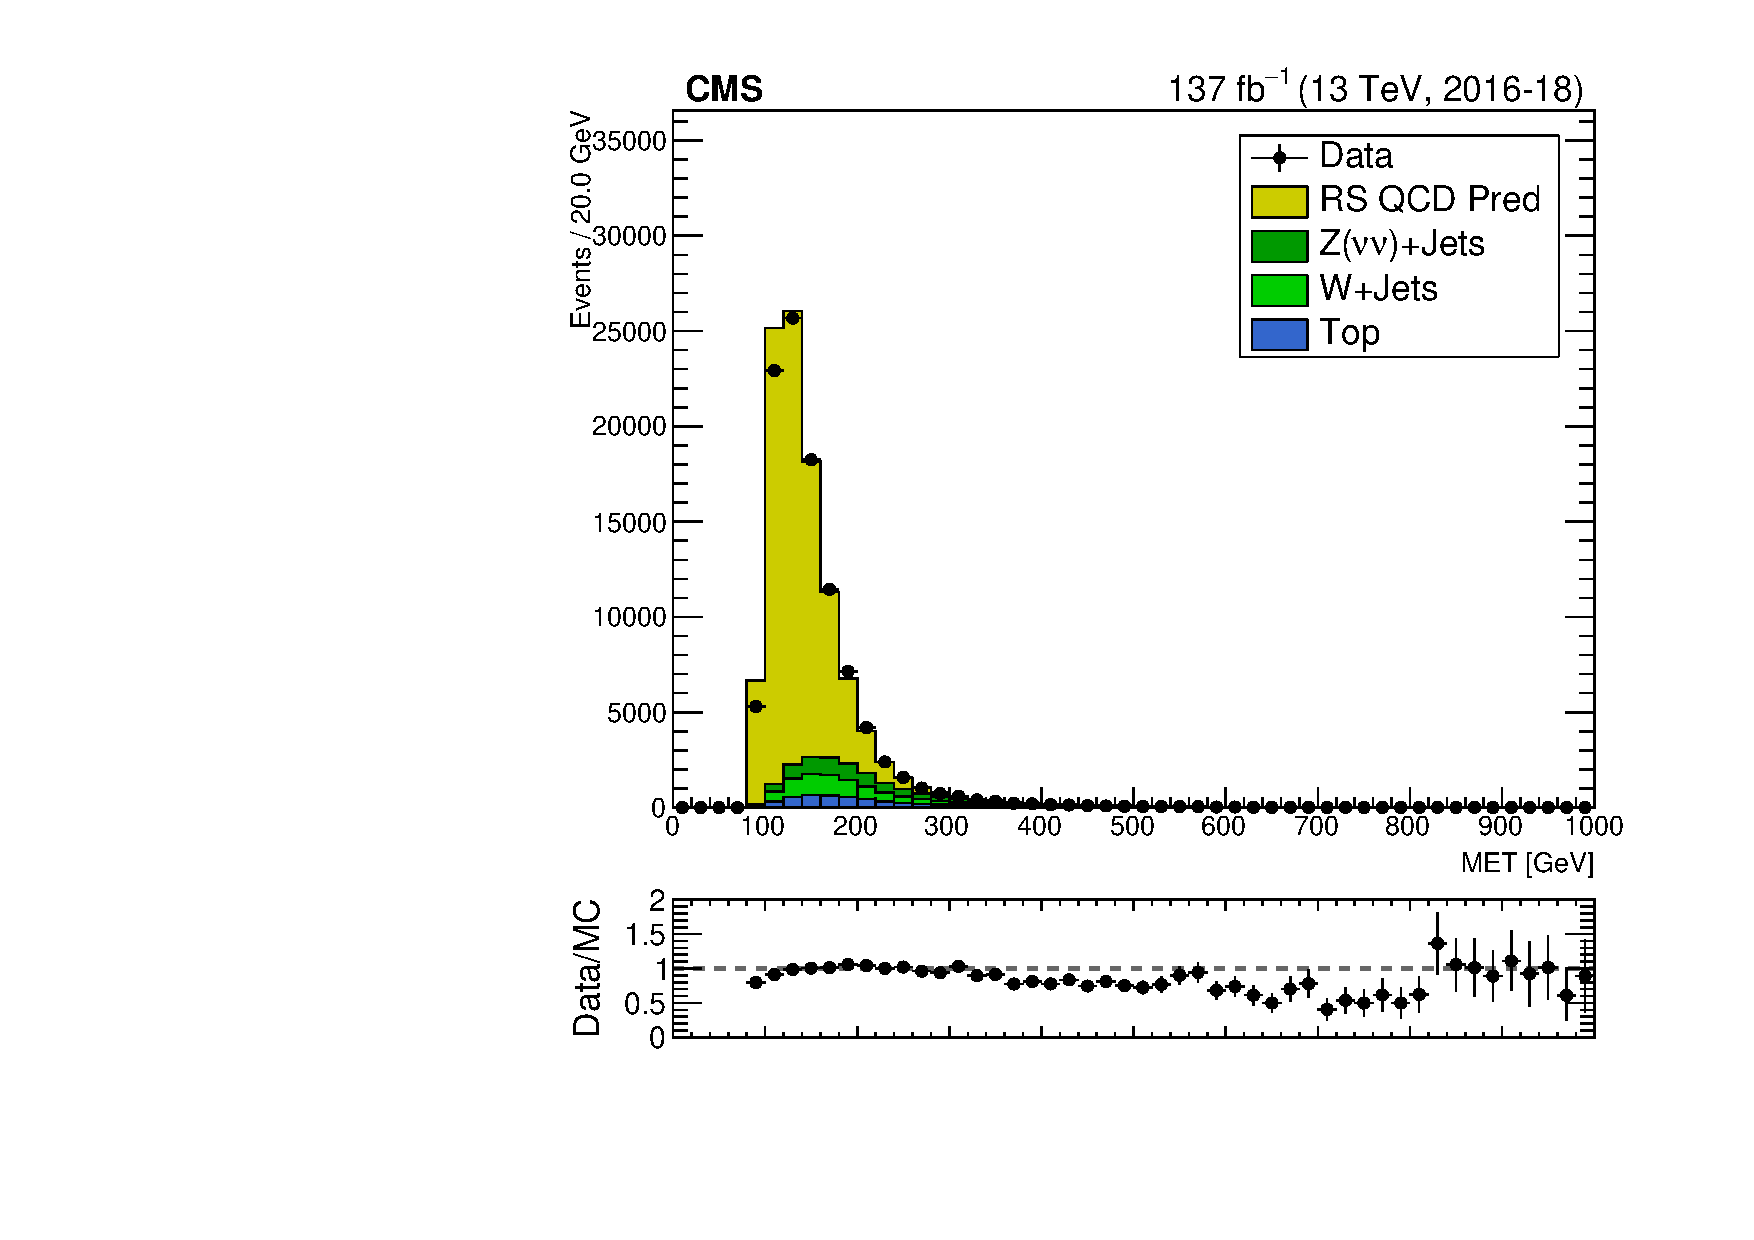
\includegraphics[width=0.46\textwidth]{figs/qcd/rs_data/c_crRSMT2SideBandInclusiveHT1200toInf_h_met.pdf}
    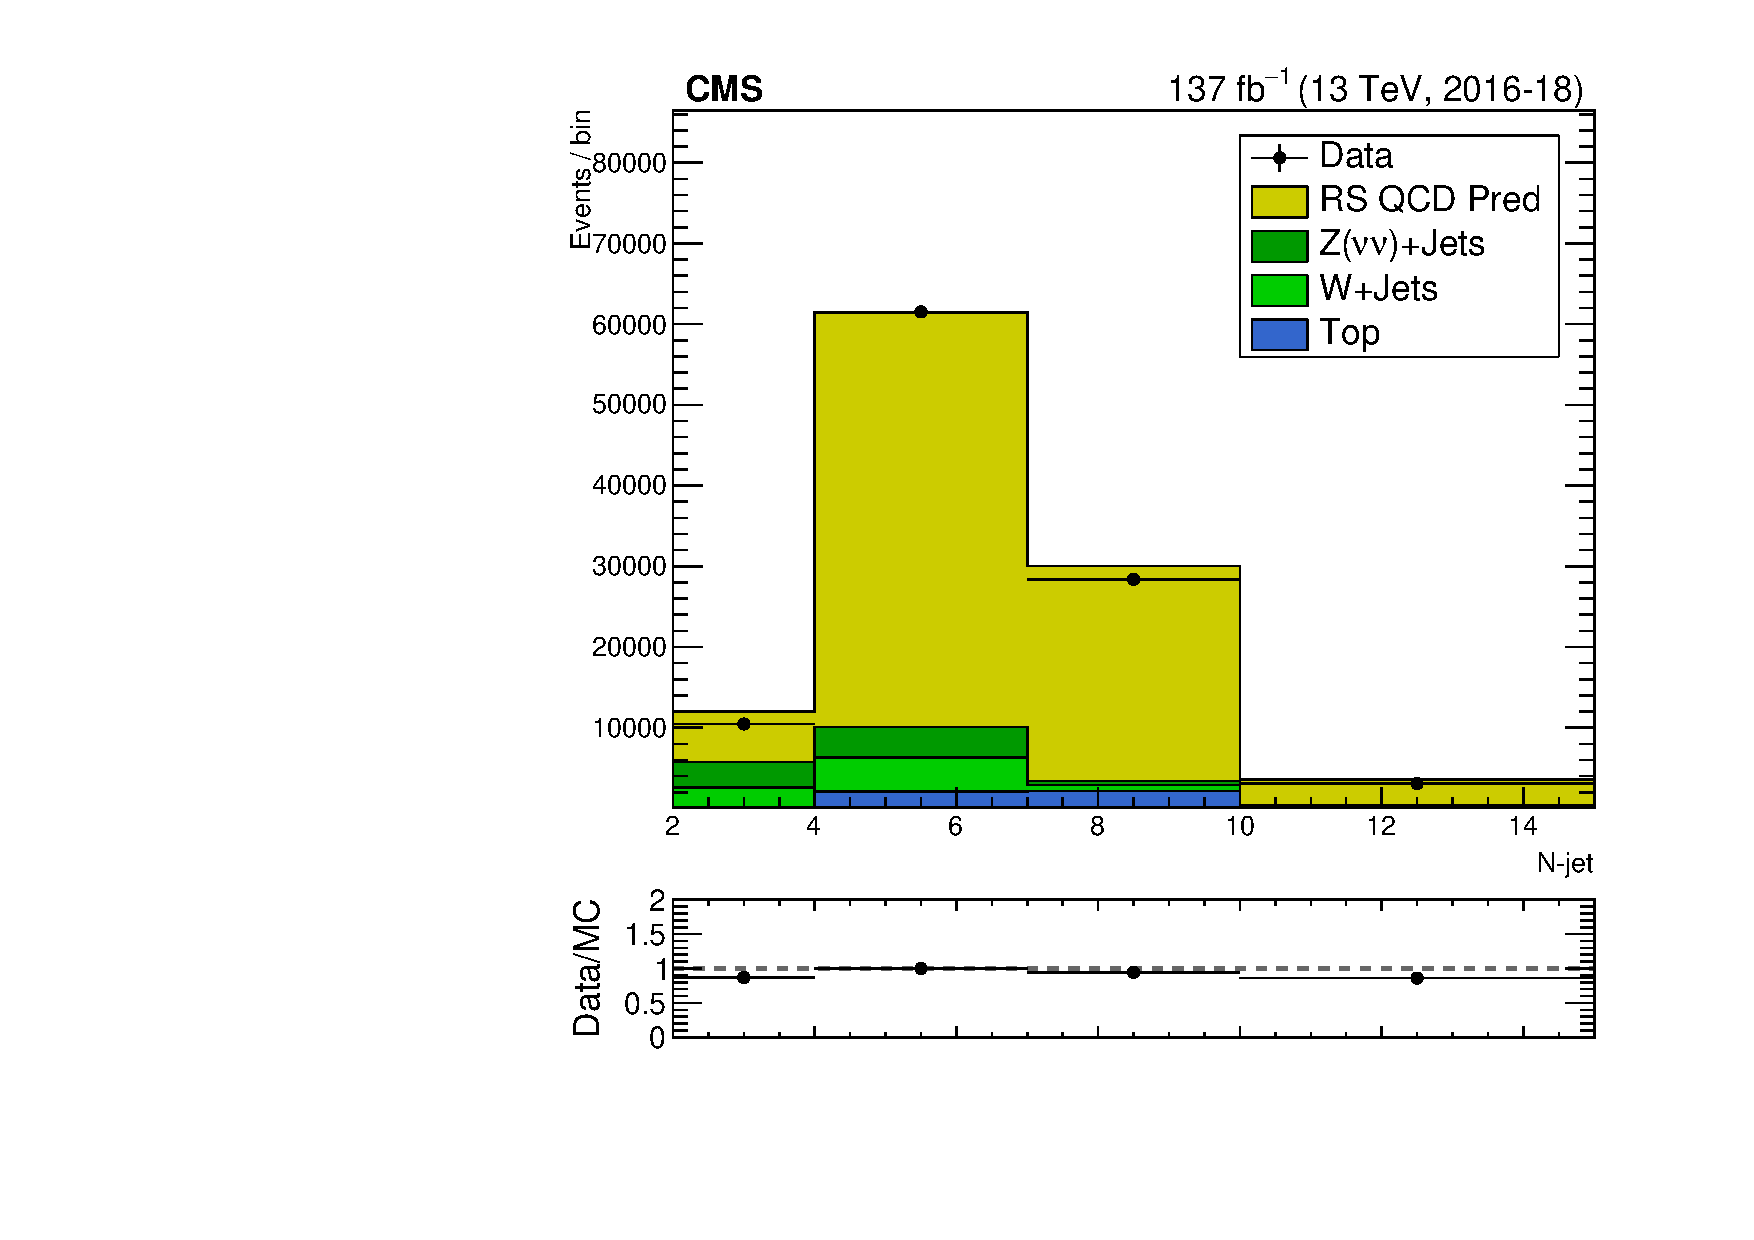
\includegraphics[width=0.46\textwidth]{figs/qcd/rs_data/c_crRSMT2SideBandInclusiveHT1200toInf_h_nJet30.pdf}
    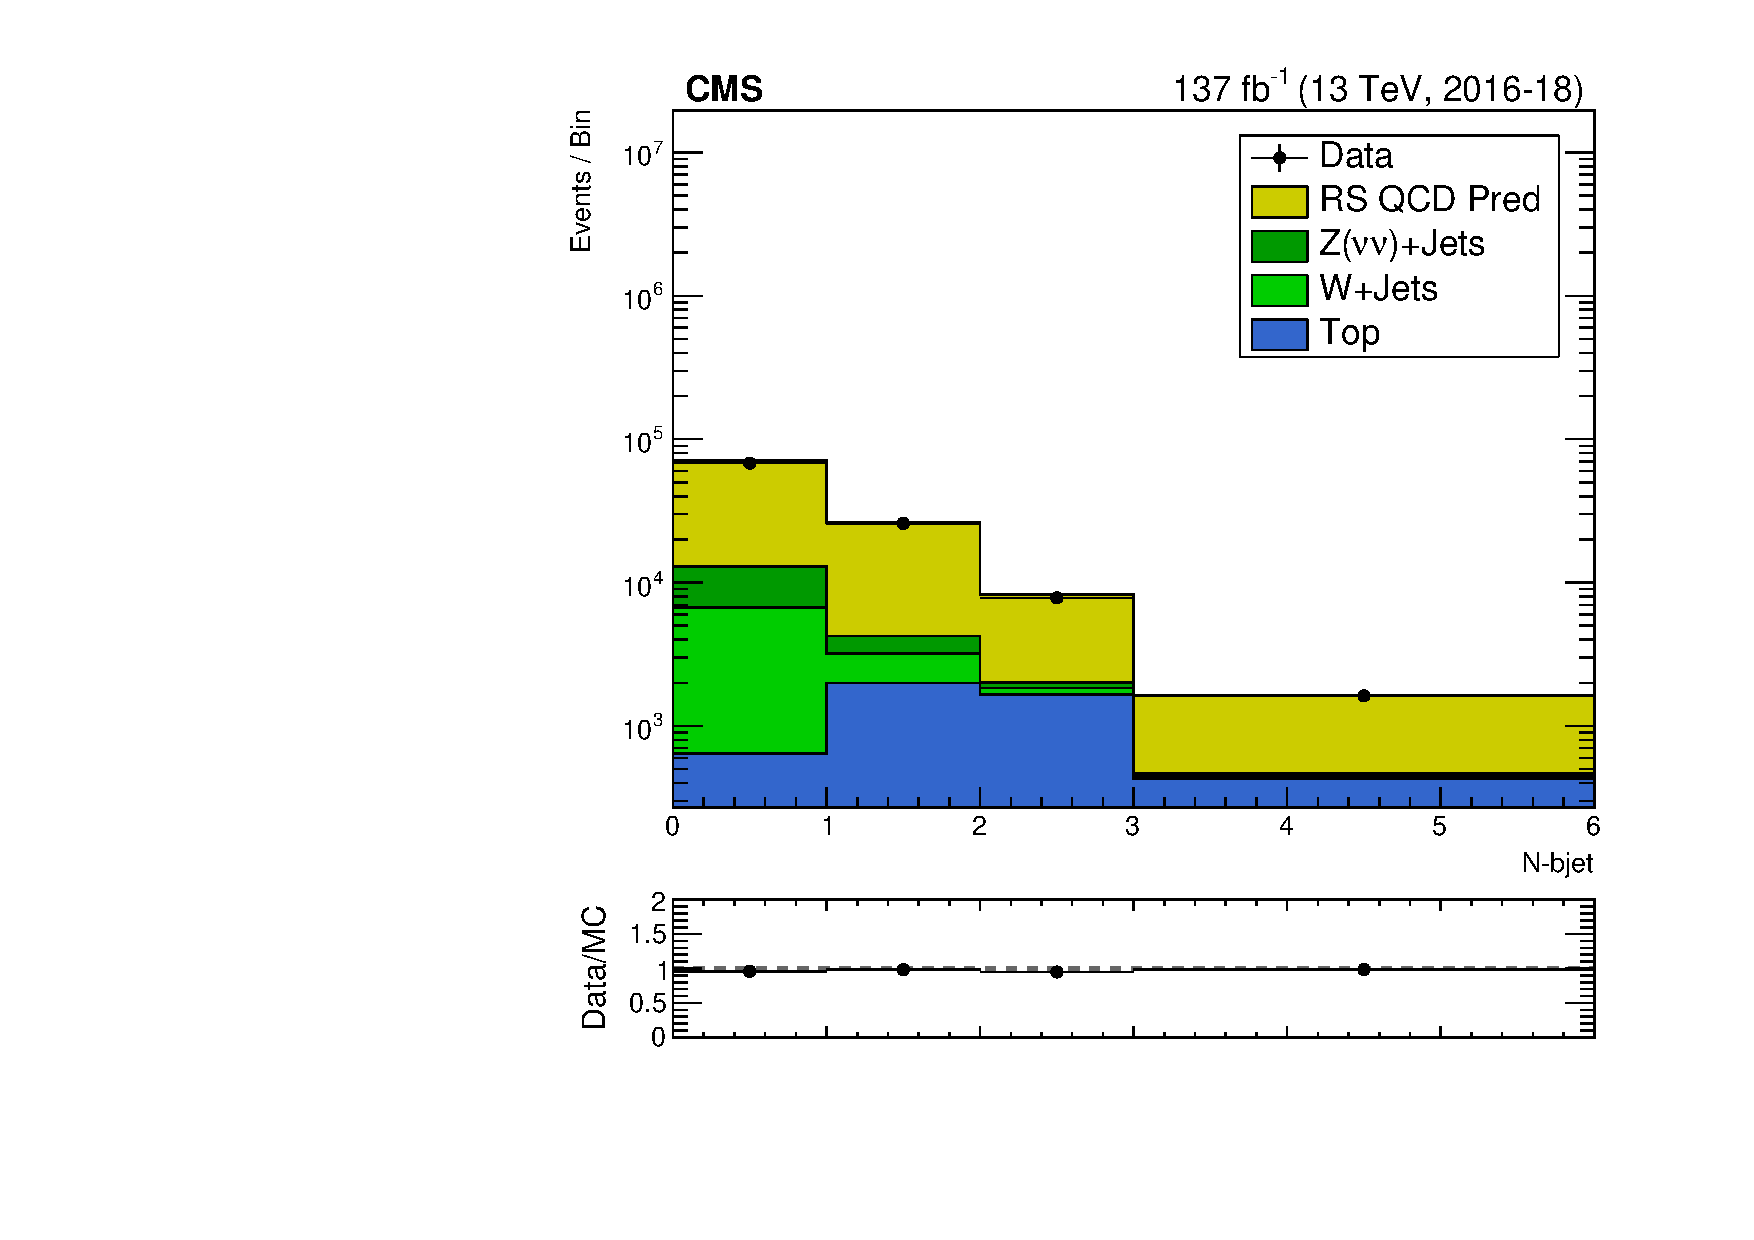
\includegraphics[width=0.46\textwidth]{figs/qcd/rs_data/c_crRSMT2SideBandInclusiveHT1200toInf_h_nBJet20.pdf}
    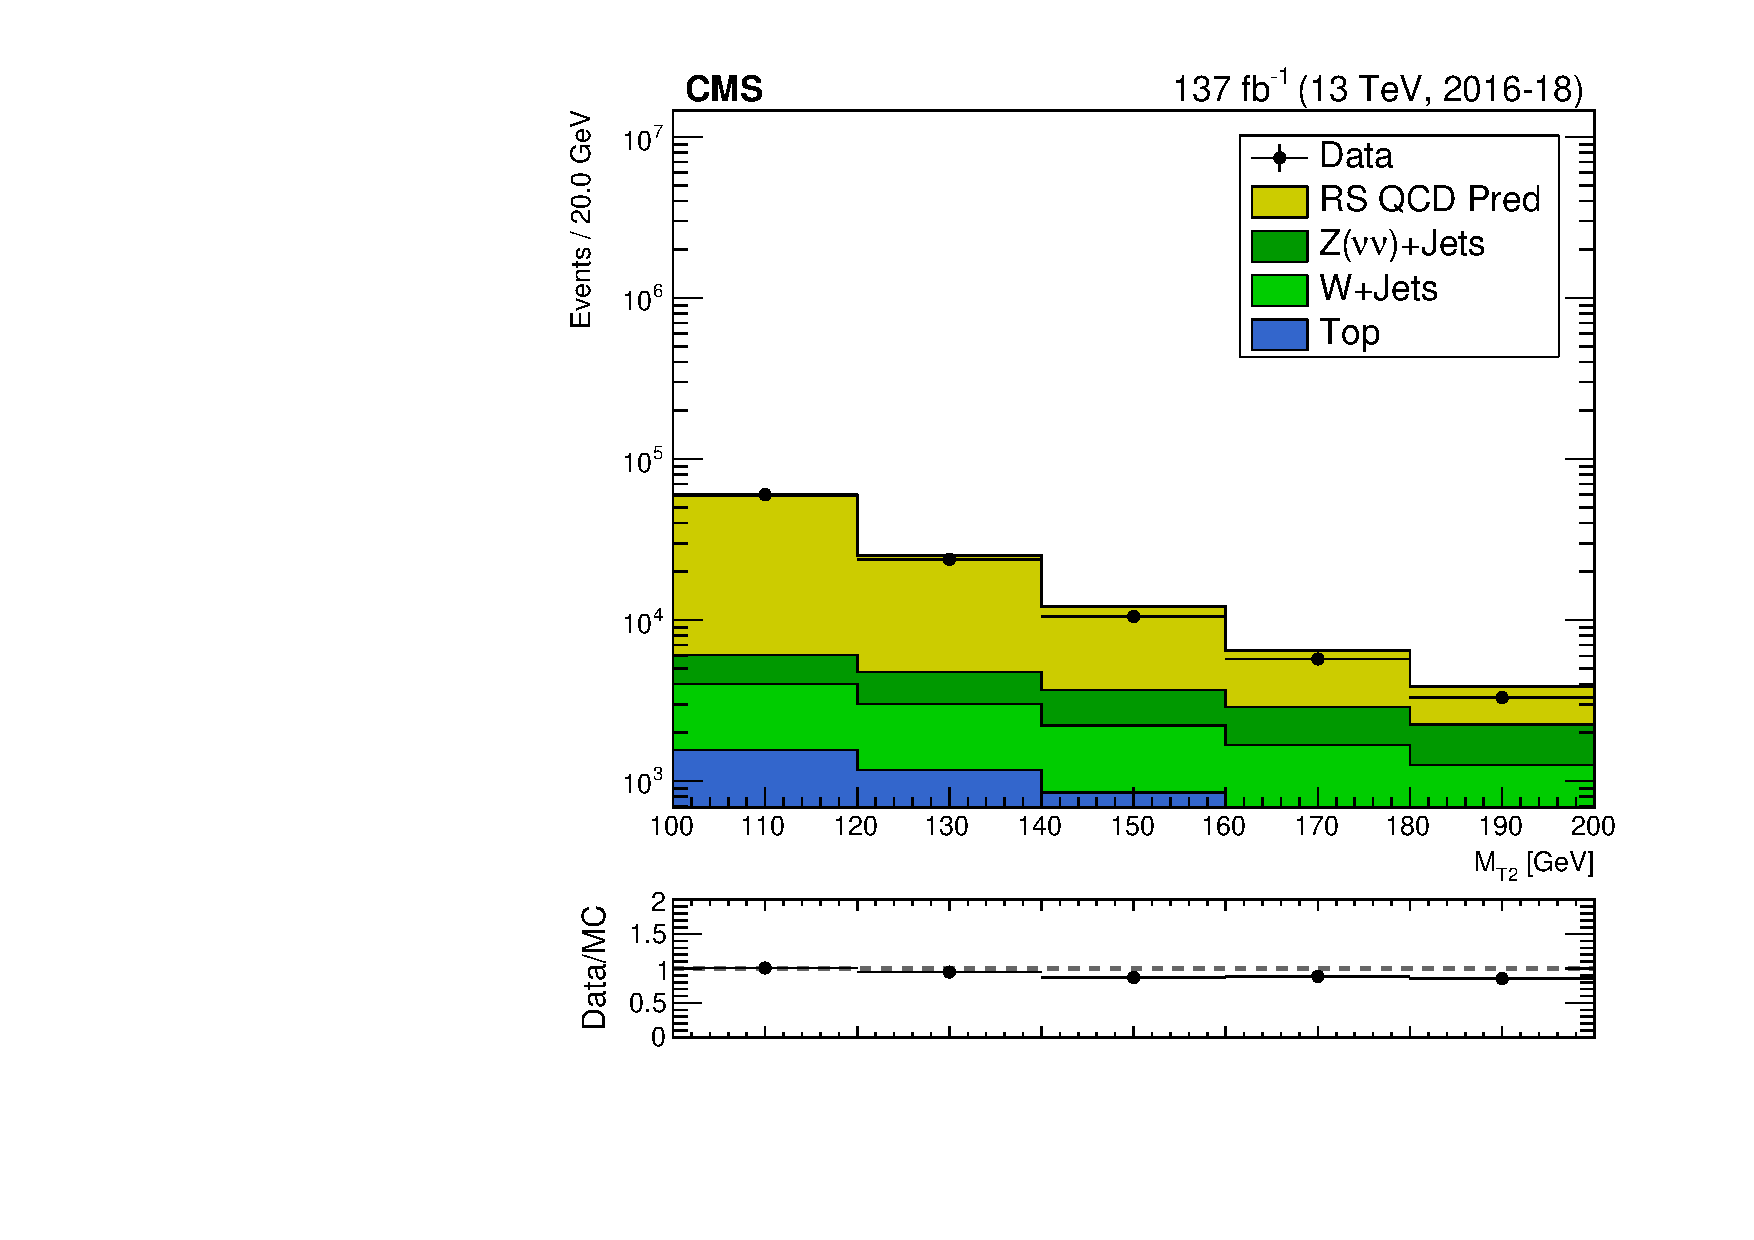
\includegraphics[width=0.46\textwidth]{figs/qcd/rs_data/c_crRSMT2SideBandInclusiveHT1200toInf_h_mt2.pdf}
    \caption{Comparison of kinematic distributions for data and background in the $\mttwo$ sideband control region ($100< \mttwo <$ 200\GeV) for $\Ht > 1200$\GeV. The QCD background is from the
             rebalance and smear data-driven prediction. Non-QCD backgrounds are taken from Monte Carlo.
            }
    \label{Fig:rs_crRSMT2SideBandInclusiveHT1200toInf}
  \end{center}
\end{figure}

\begin{figure}[!htbp]
  \begin{center}
    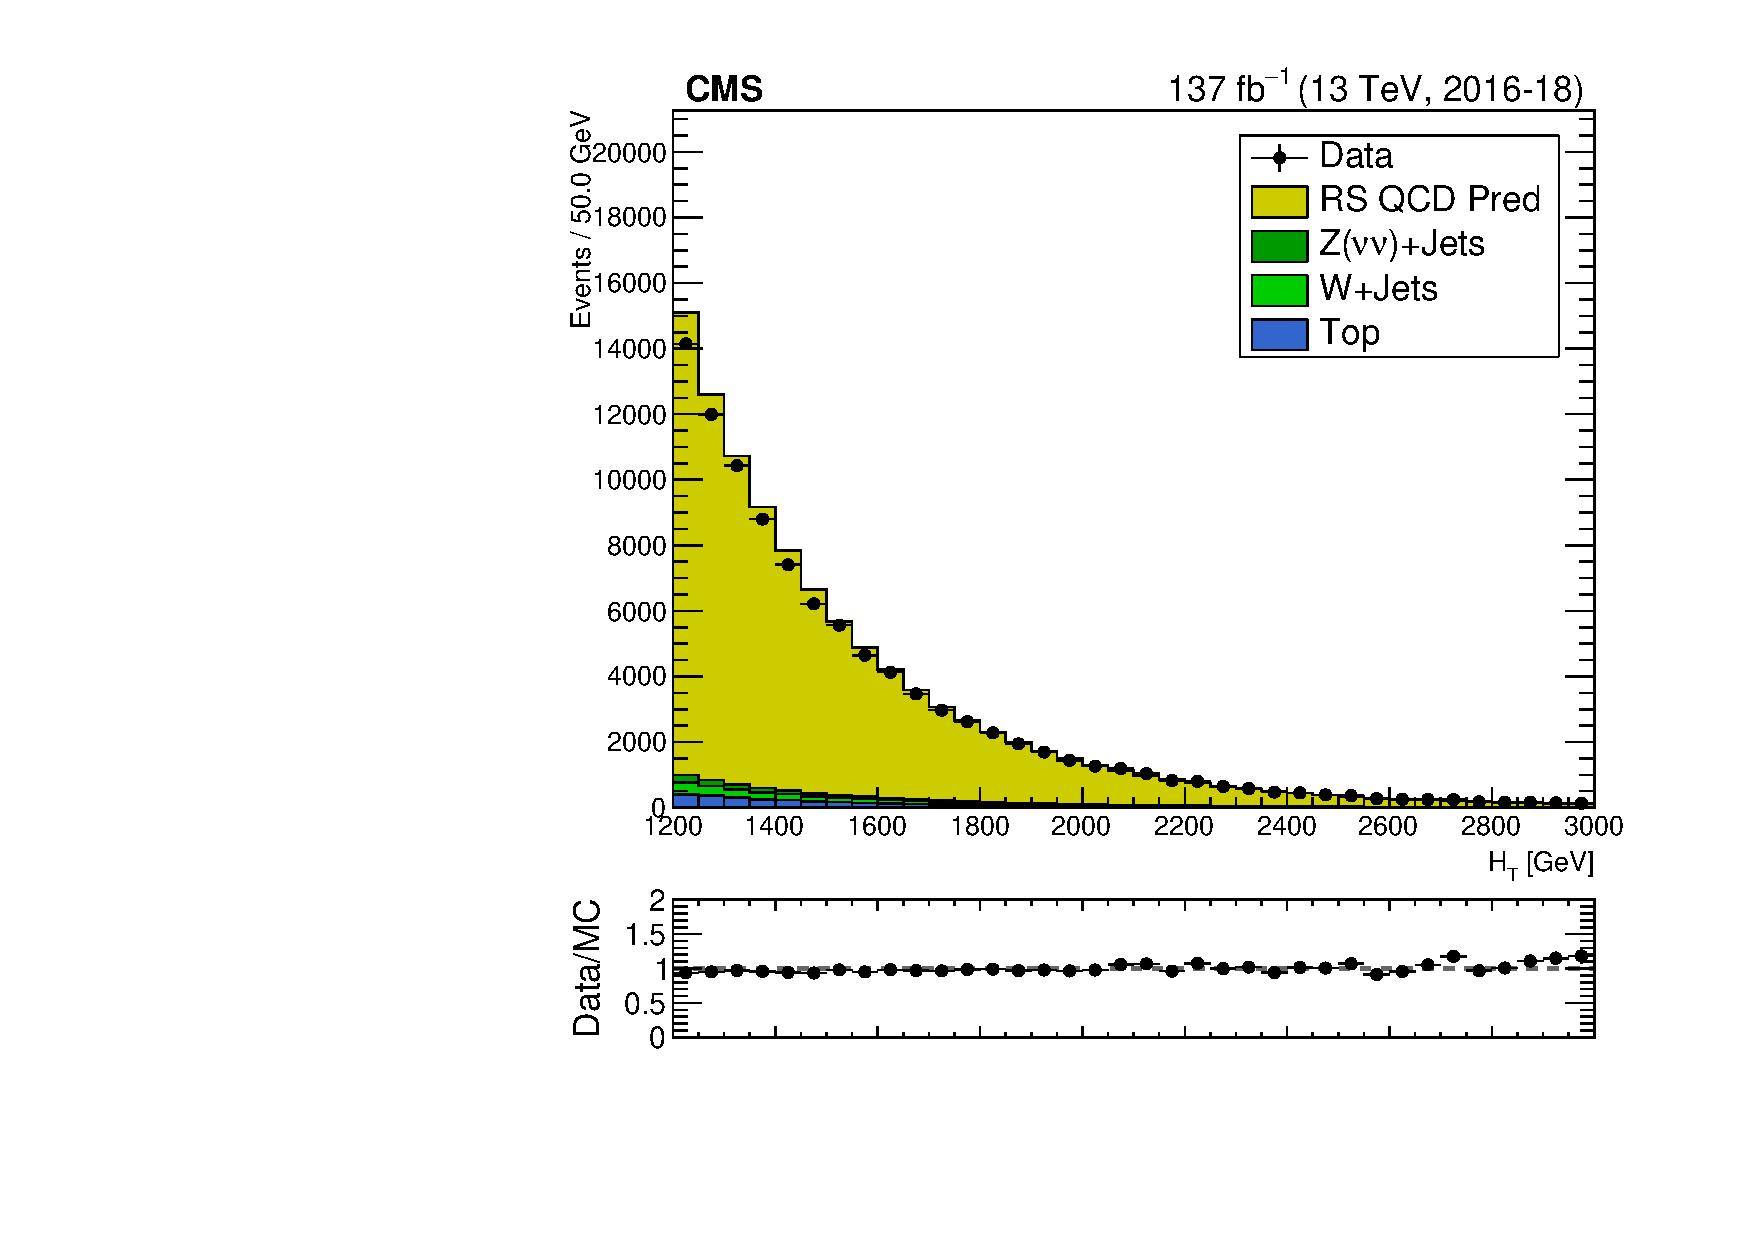
\includegraphics[width=0.46\textwidth]{figs/qcd/rs_data/c_crRSDPhiMT2InclusiveHT1200toInf_h_ht.pdf}
    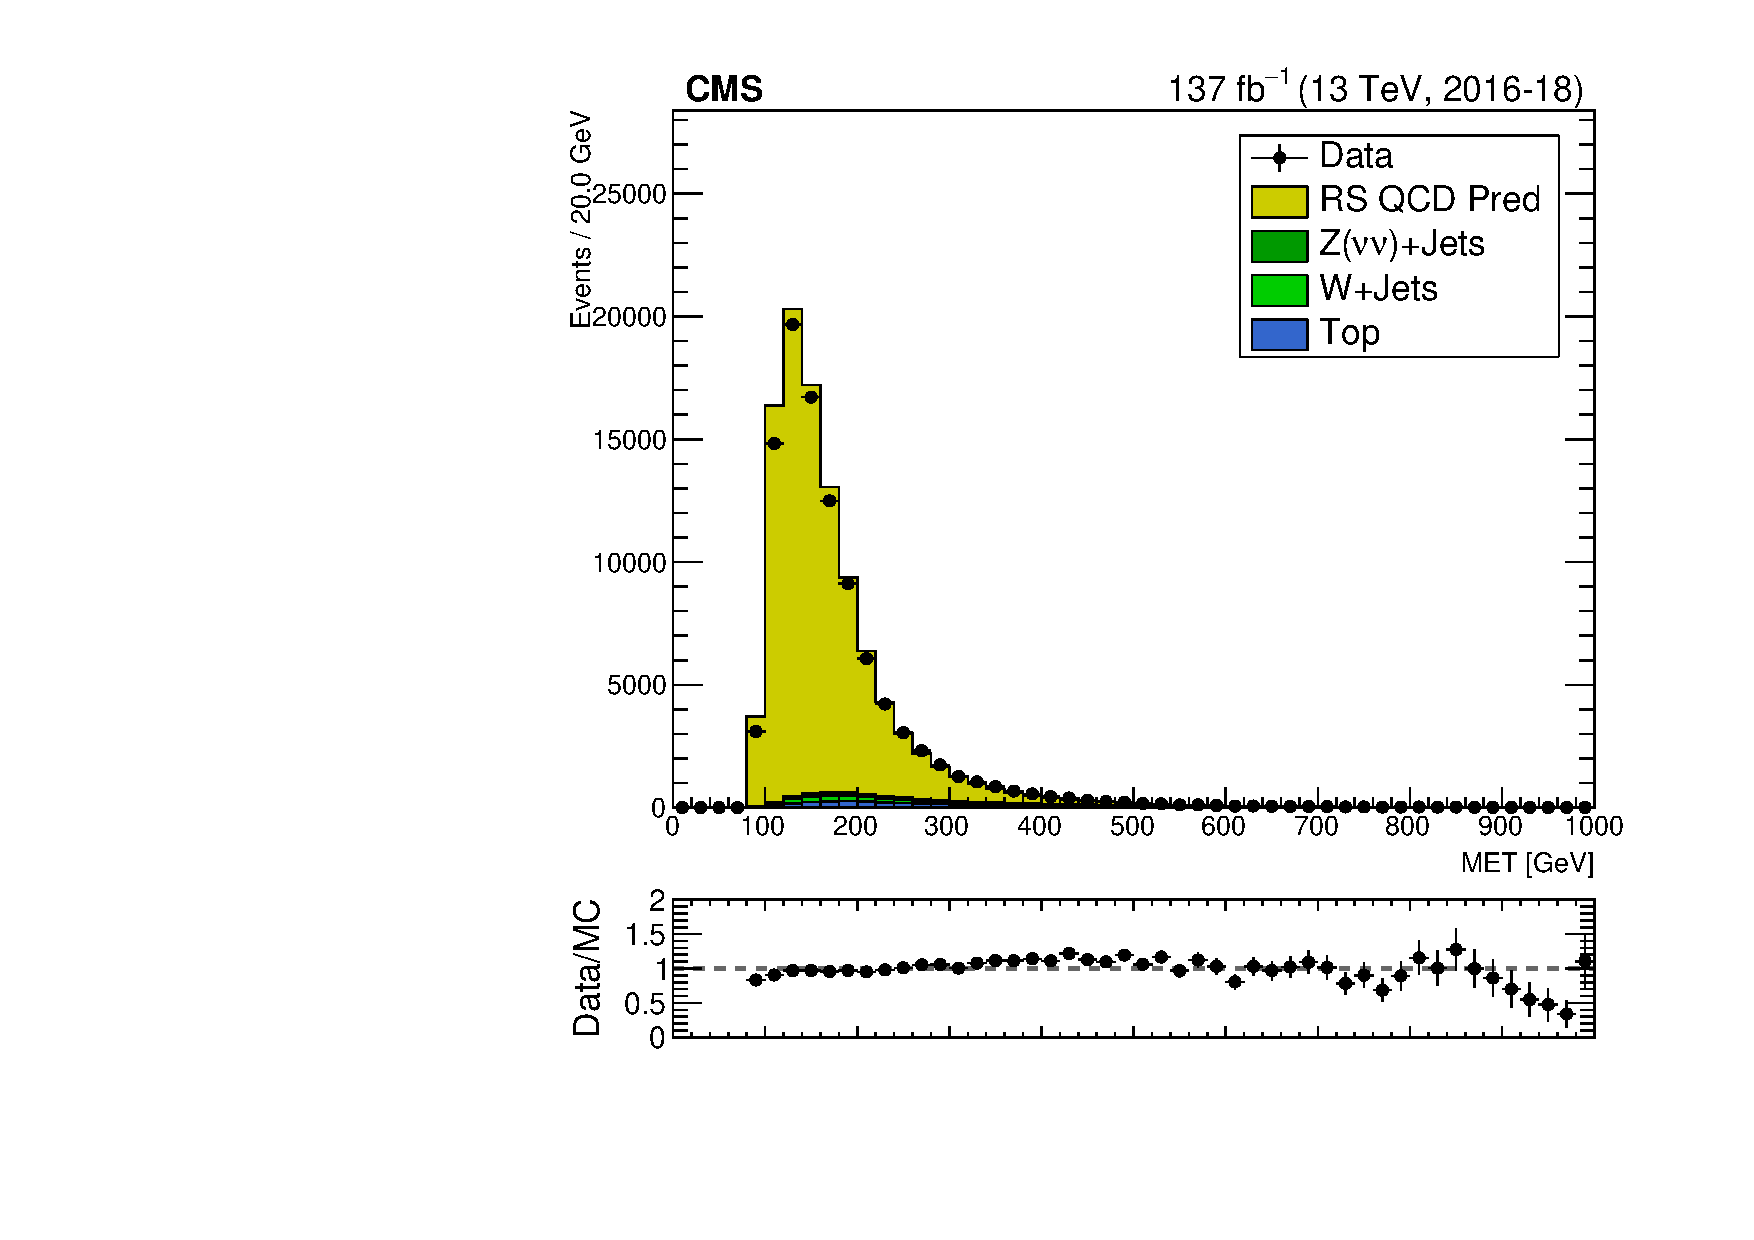
\includegraphics[width=0.46\textwidth]{figs/qcd/rs_data/c_crRSDPhiMT2InclusiveHT1200toInf_h_met.pdf}
    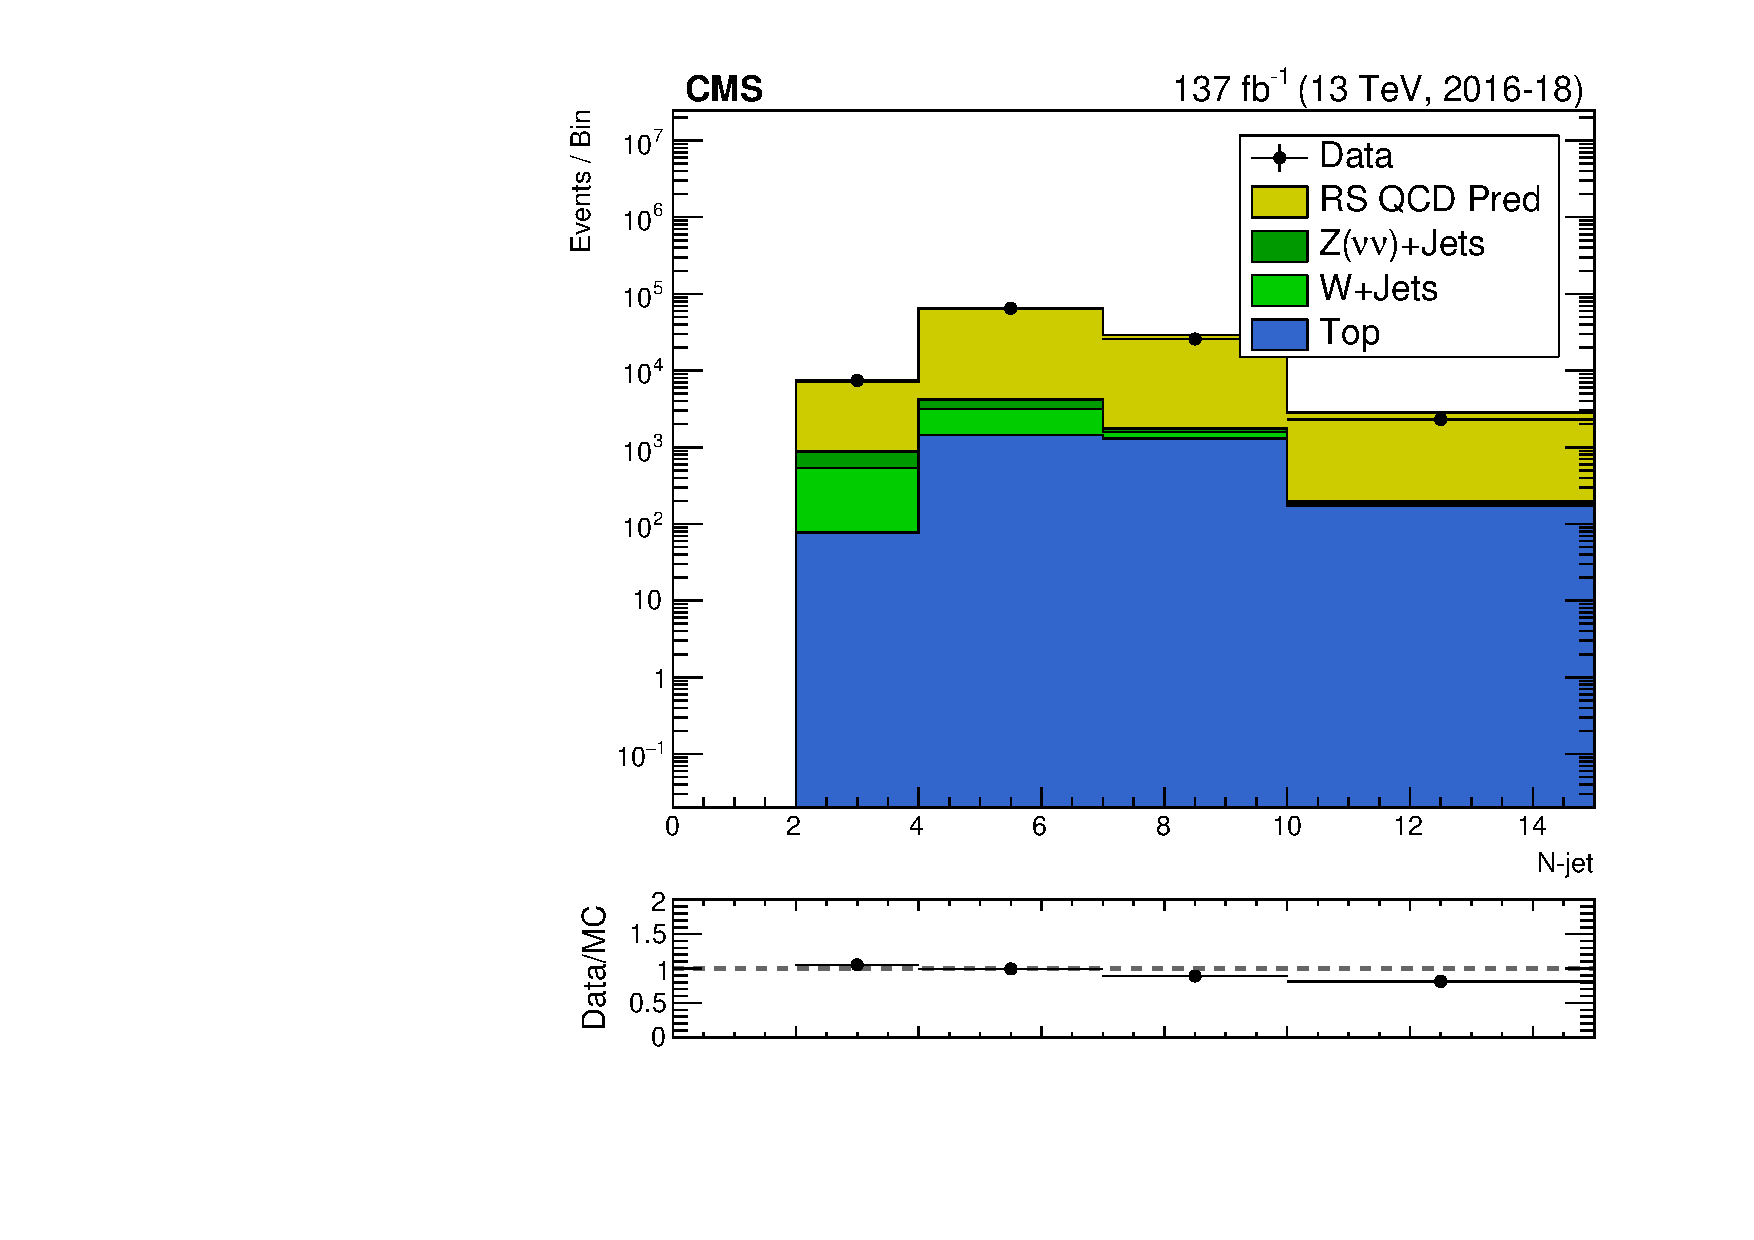
\includegraphics[width=0.46\textwidth]{figs/qcd/rs_data/c_crRSDPhiMT2InclusiveHT1200toInf_h_nJet30.pdf}
    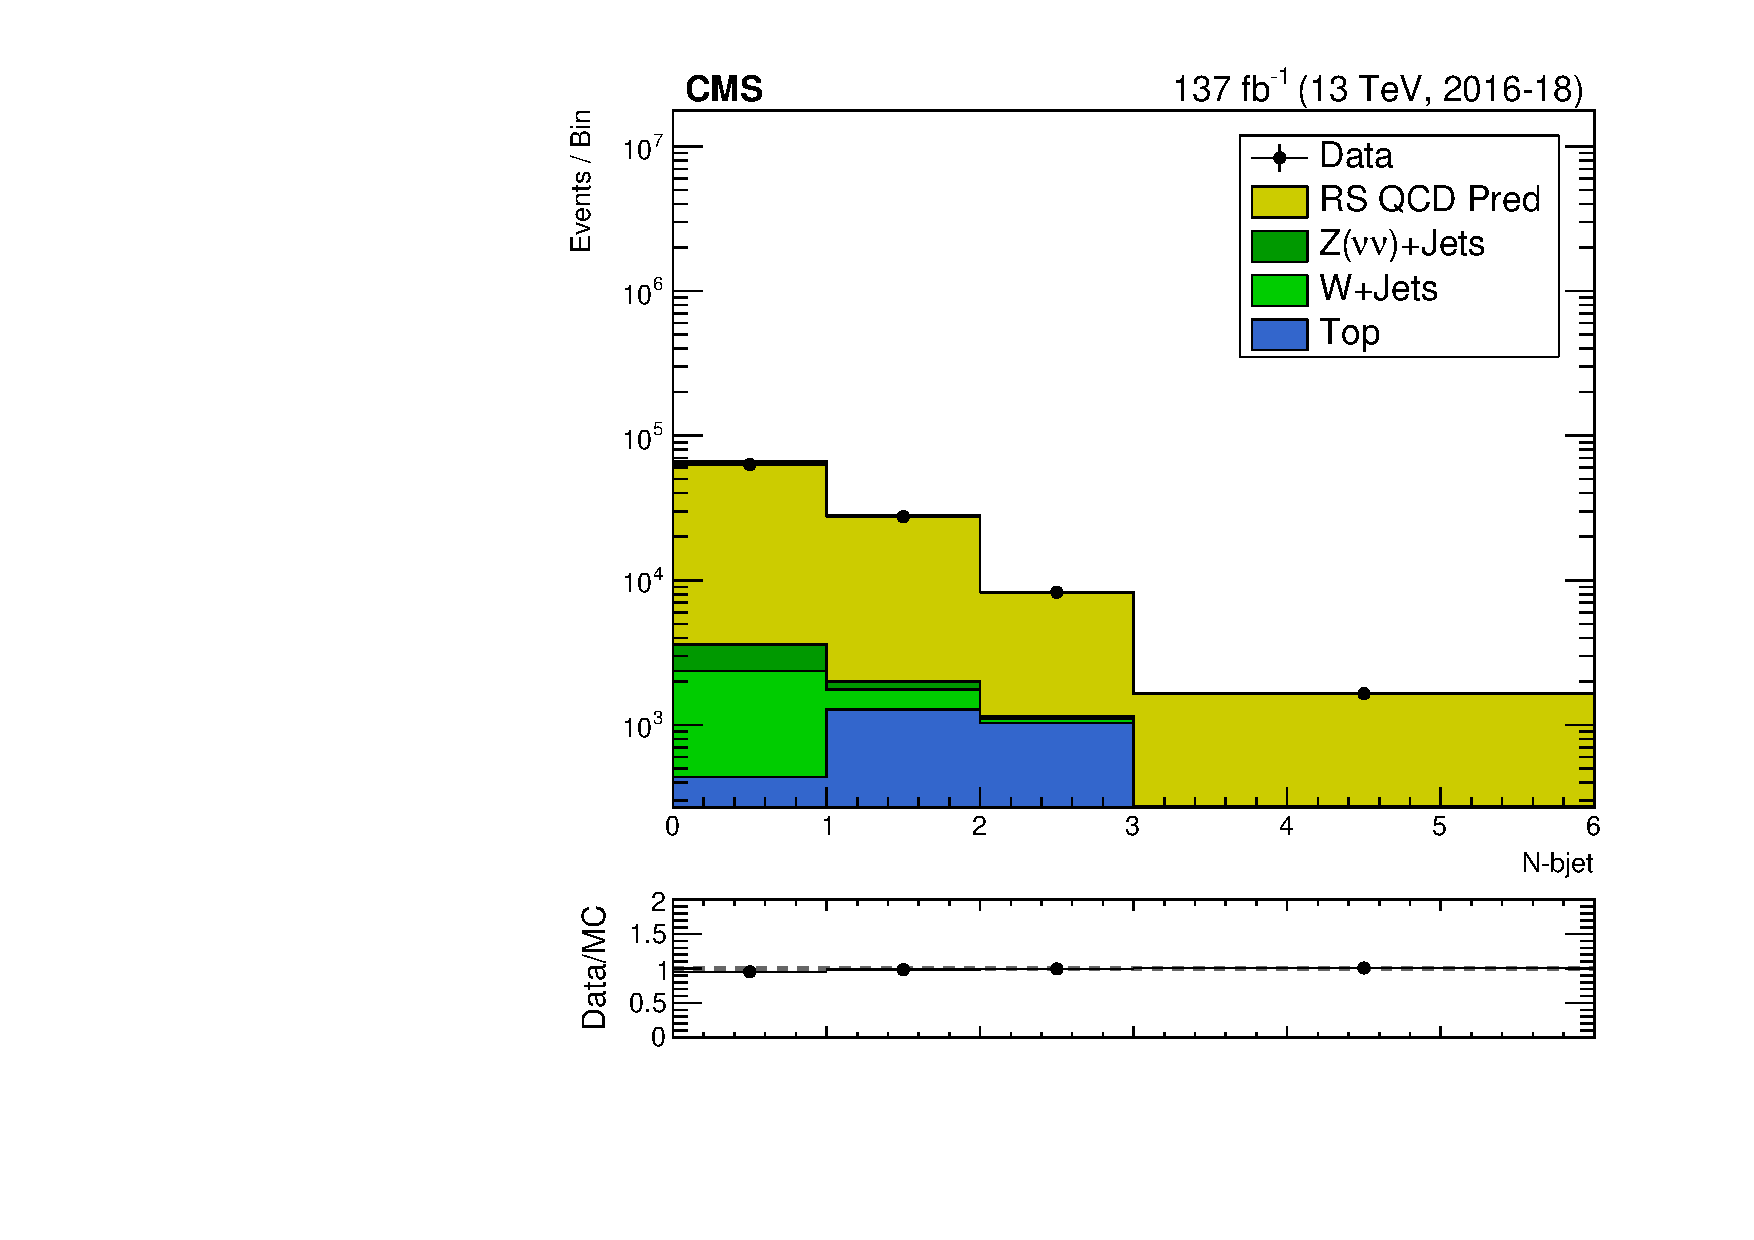
\includegraphics[width=0.46\textwidth]{figs/qcd/rs_data/c_crRSDPhiMT2InclusiveHT1200toInf_h_nBJet20.pdf}
    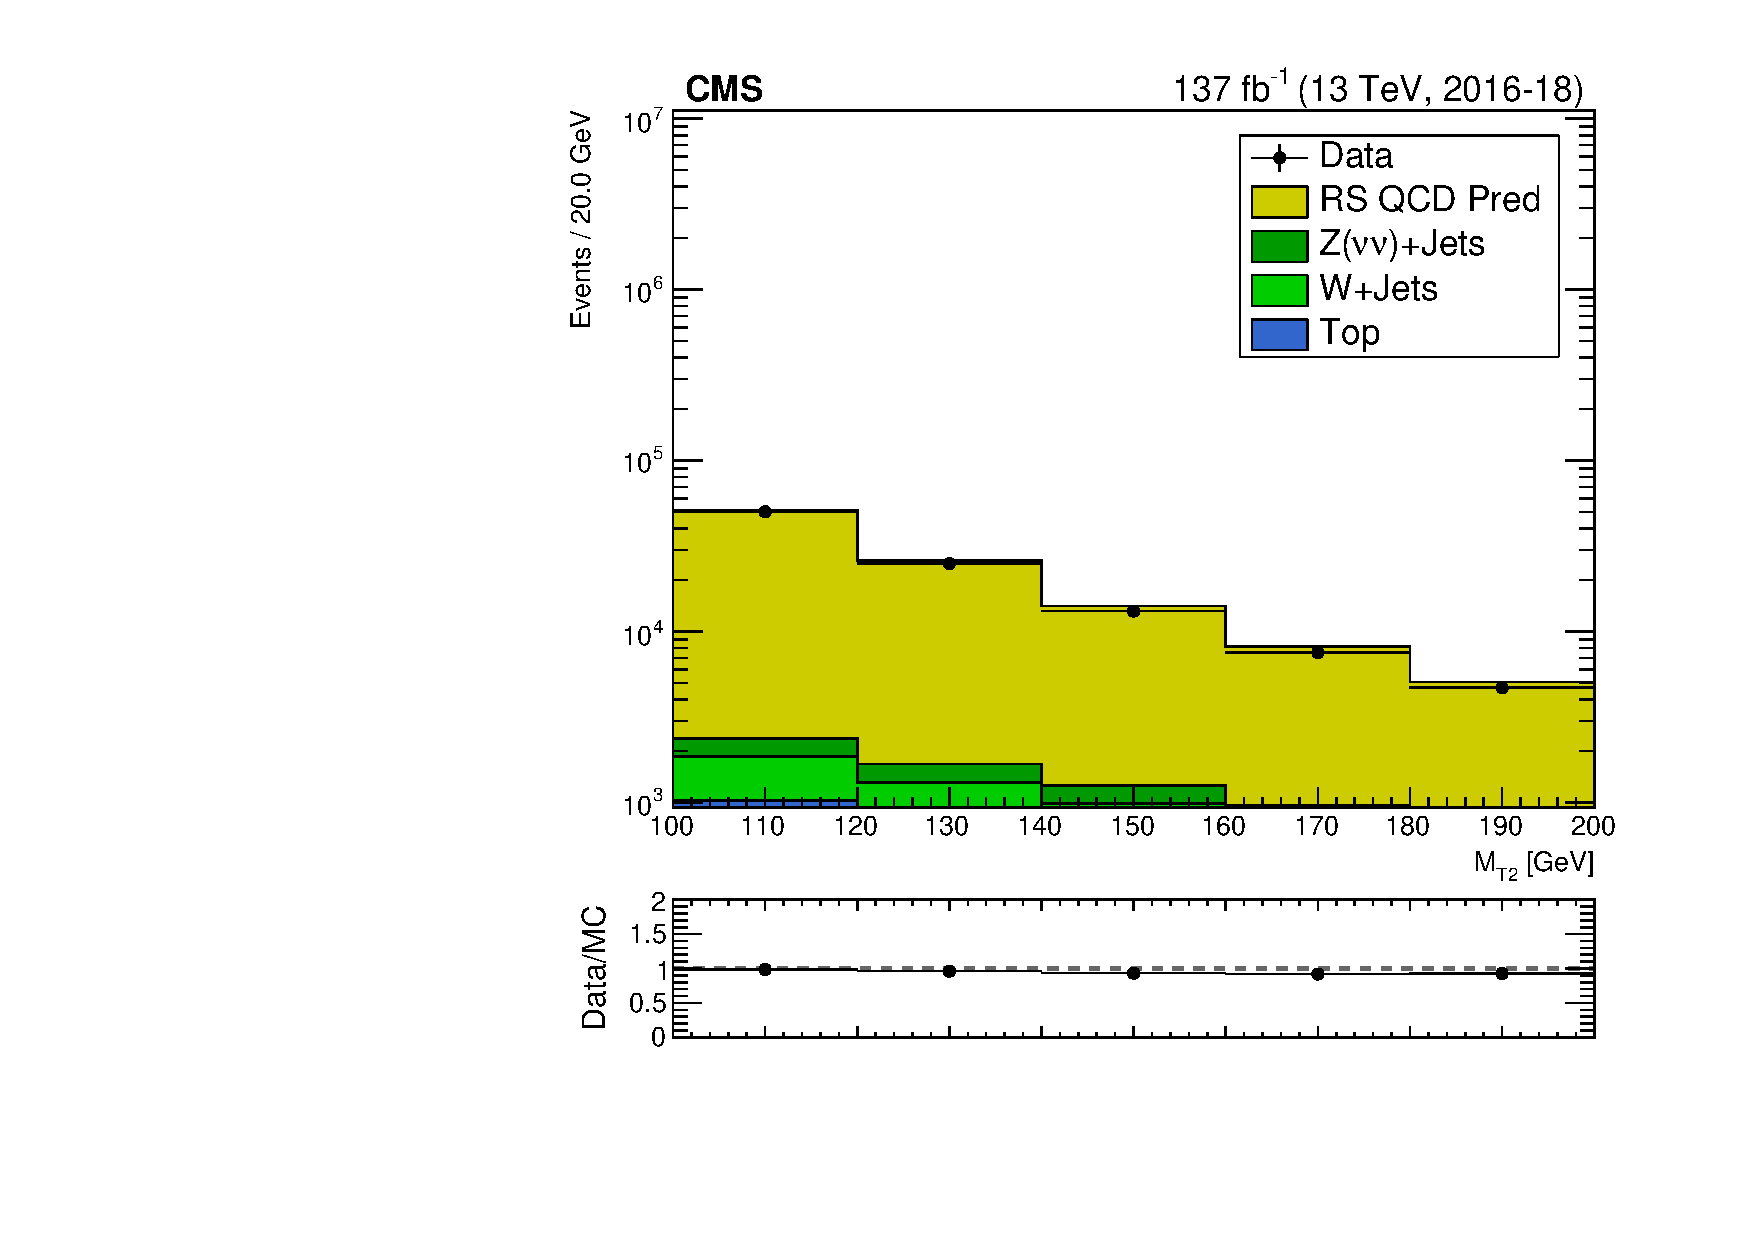
\includegraphics[width=0.46\textwidth]{figs/qcd/rs_data/c_crRSDPhiMT2InclusiveHT1200toInf_h_mt2.pdf}
    \caption{Comparison of kinematic distributions for data and background in the $\mttwo$ sideband + inverted $\dpmin$ control region for $\Ht > 1200$\GeV. The QCD background is from the
             rebalance and smear data-driven prediction. Non-QCD backgrounds are taken from Monte Carlo.
            }
    \label{Fig:rs_crRSDPhiMT2InclusiveHT1200toInf}
  \end{center}
\end{figure}

\begin{figure}[!htbp]
  \begin{center}
    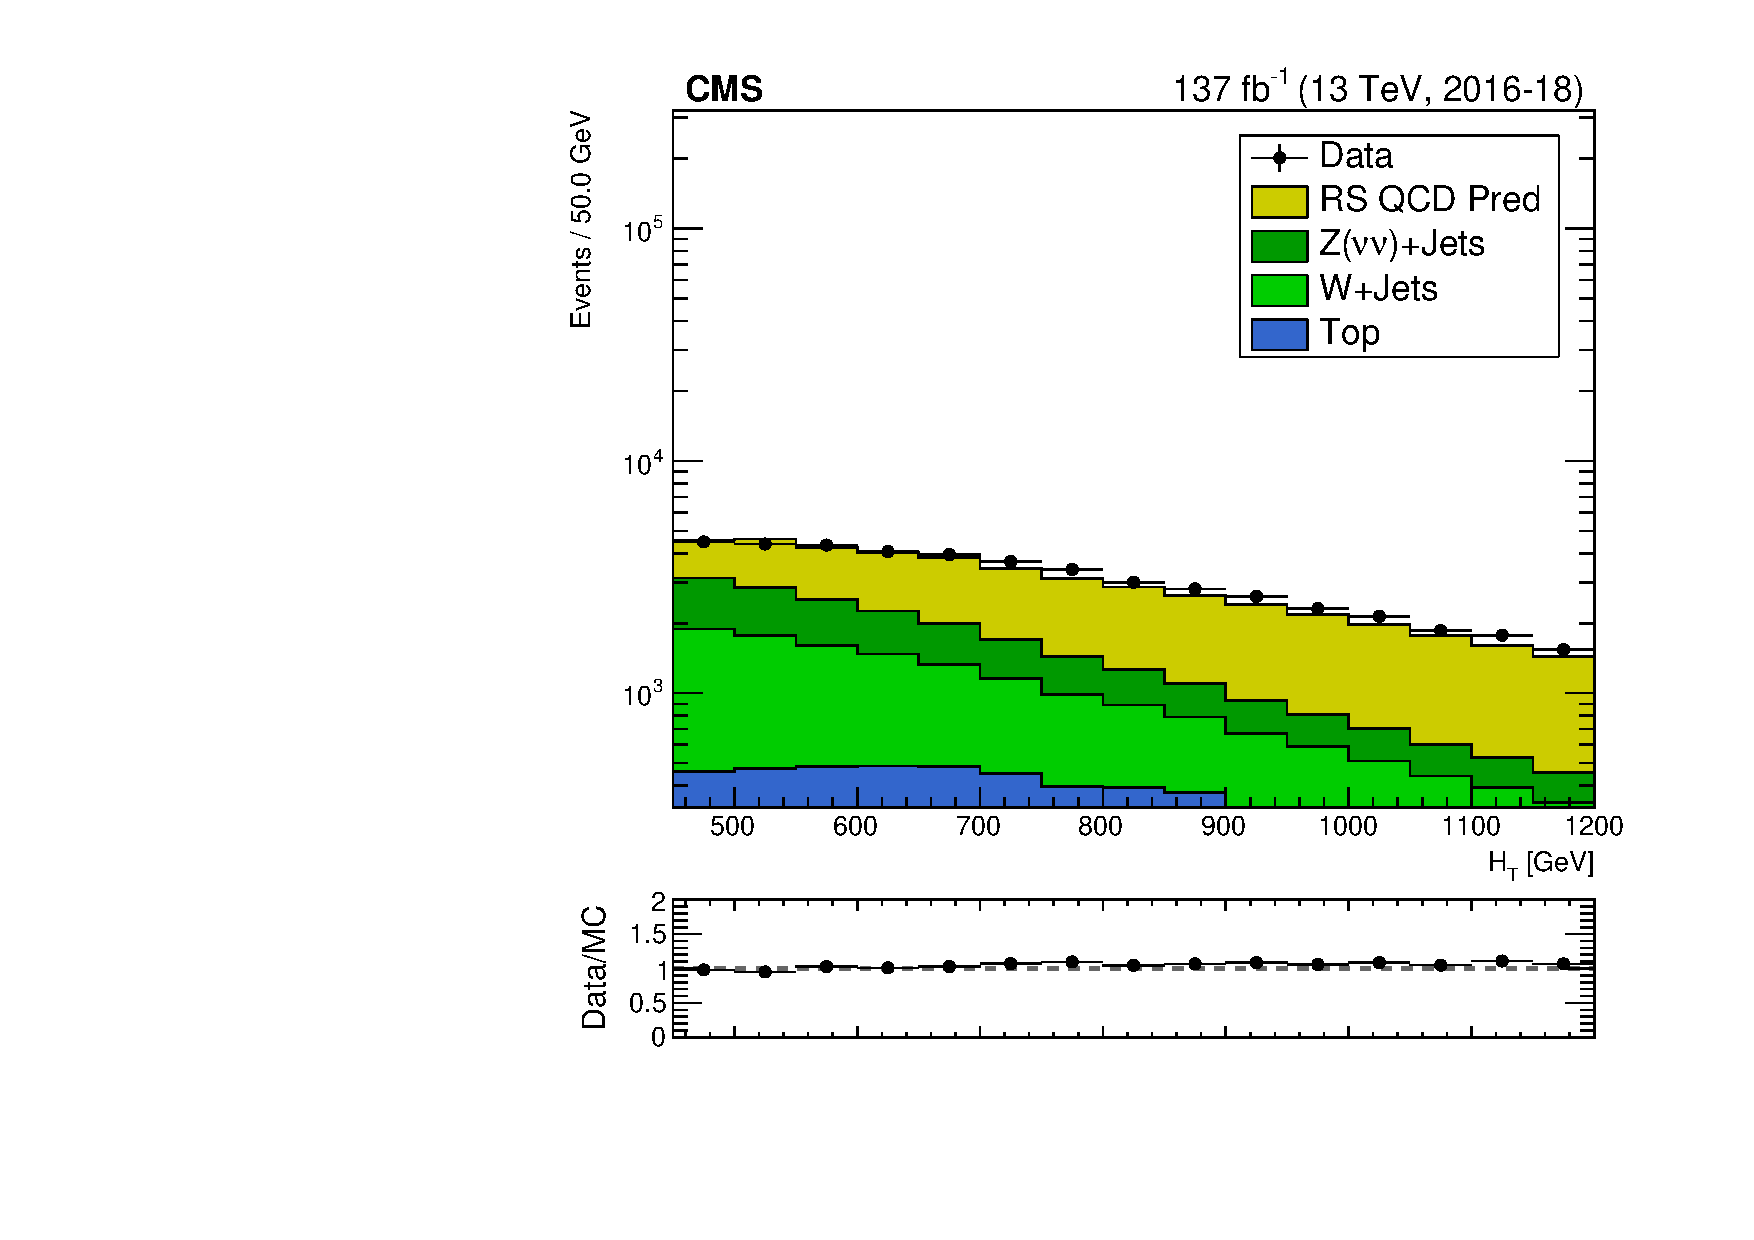
\includegraphics[width=0.46\textwidth]{figs/qcd/rs_data/c_crRSDPhiMT2InclusiveHT450to1200_h_ht.pdf}
    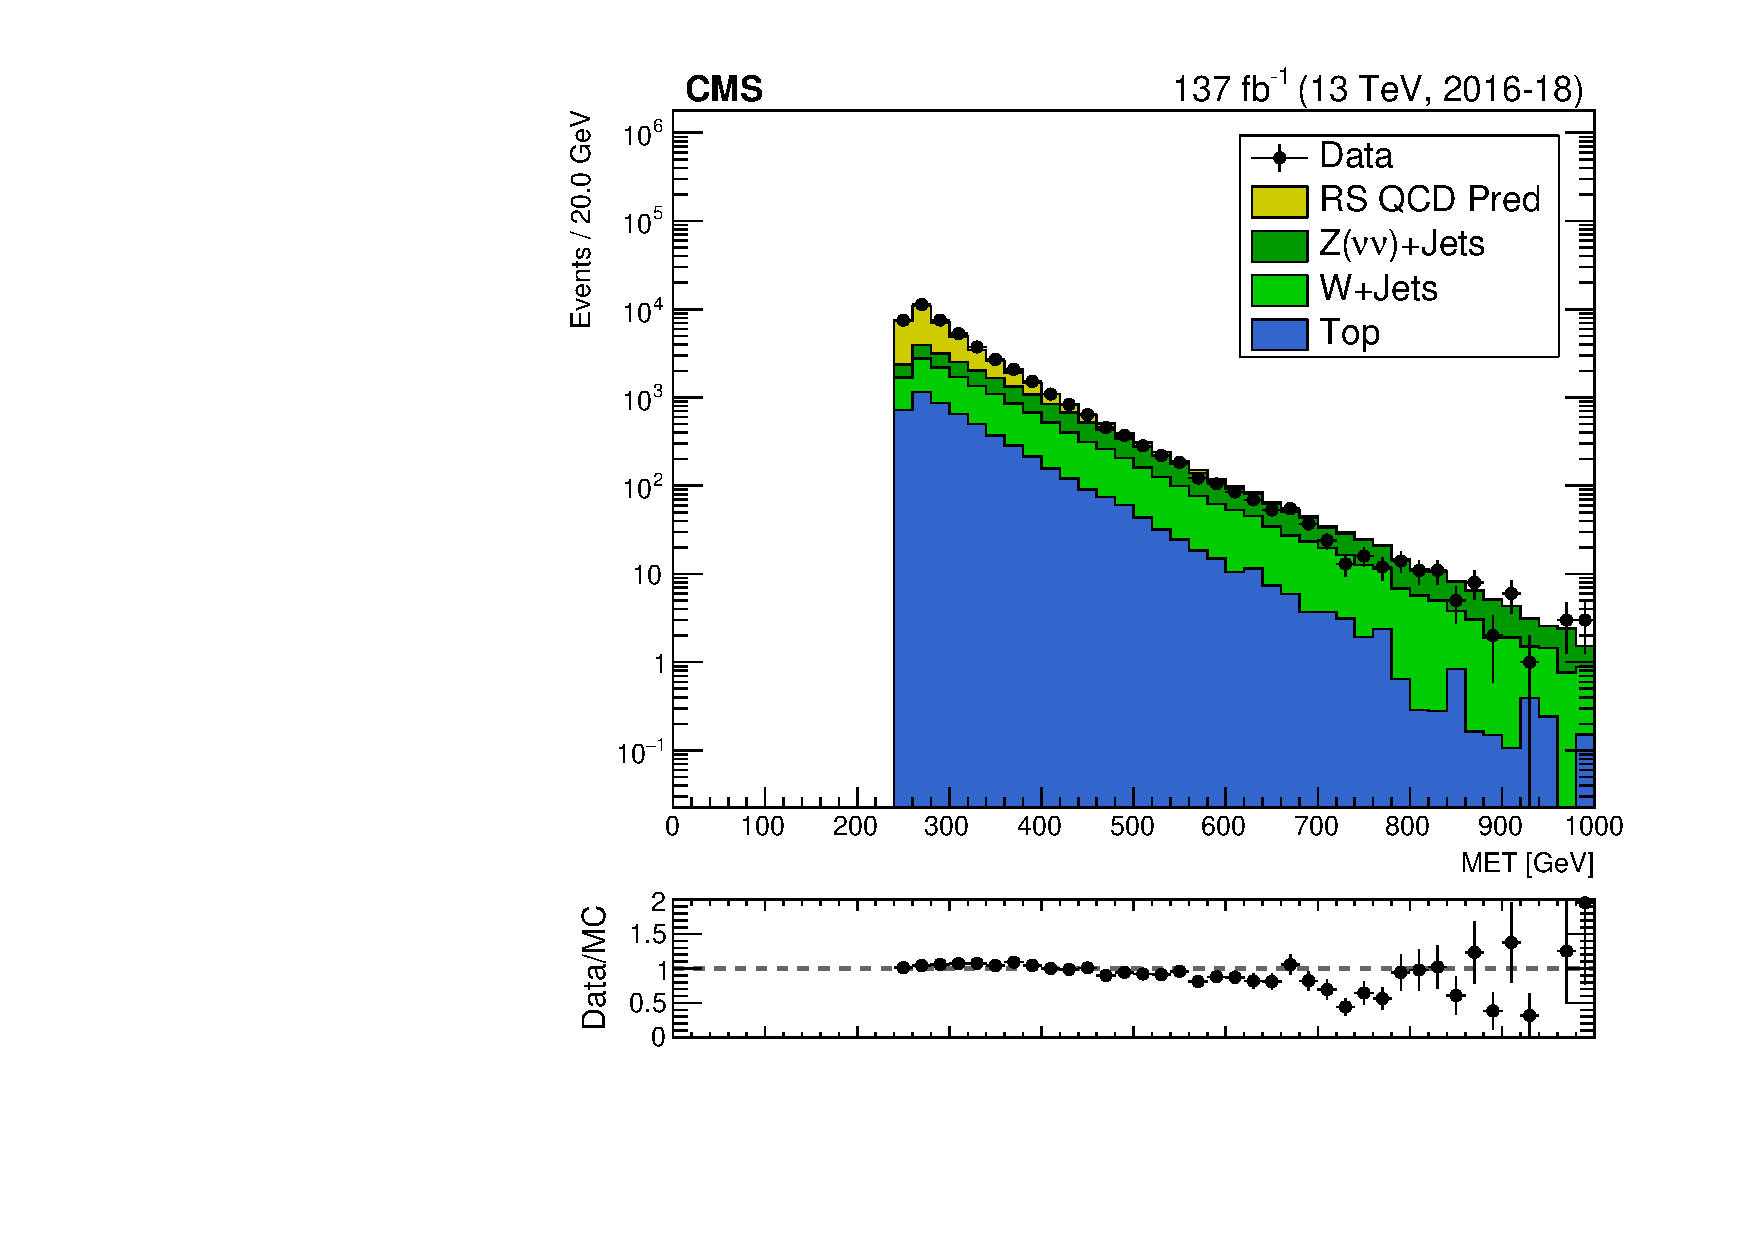
\includegraphics[width=0.46\textwidth]{figs/qcd/rs_data/c_crRSDPhiMT2InclusiveHT450to1200_h_met.pdf}
    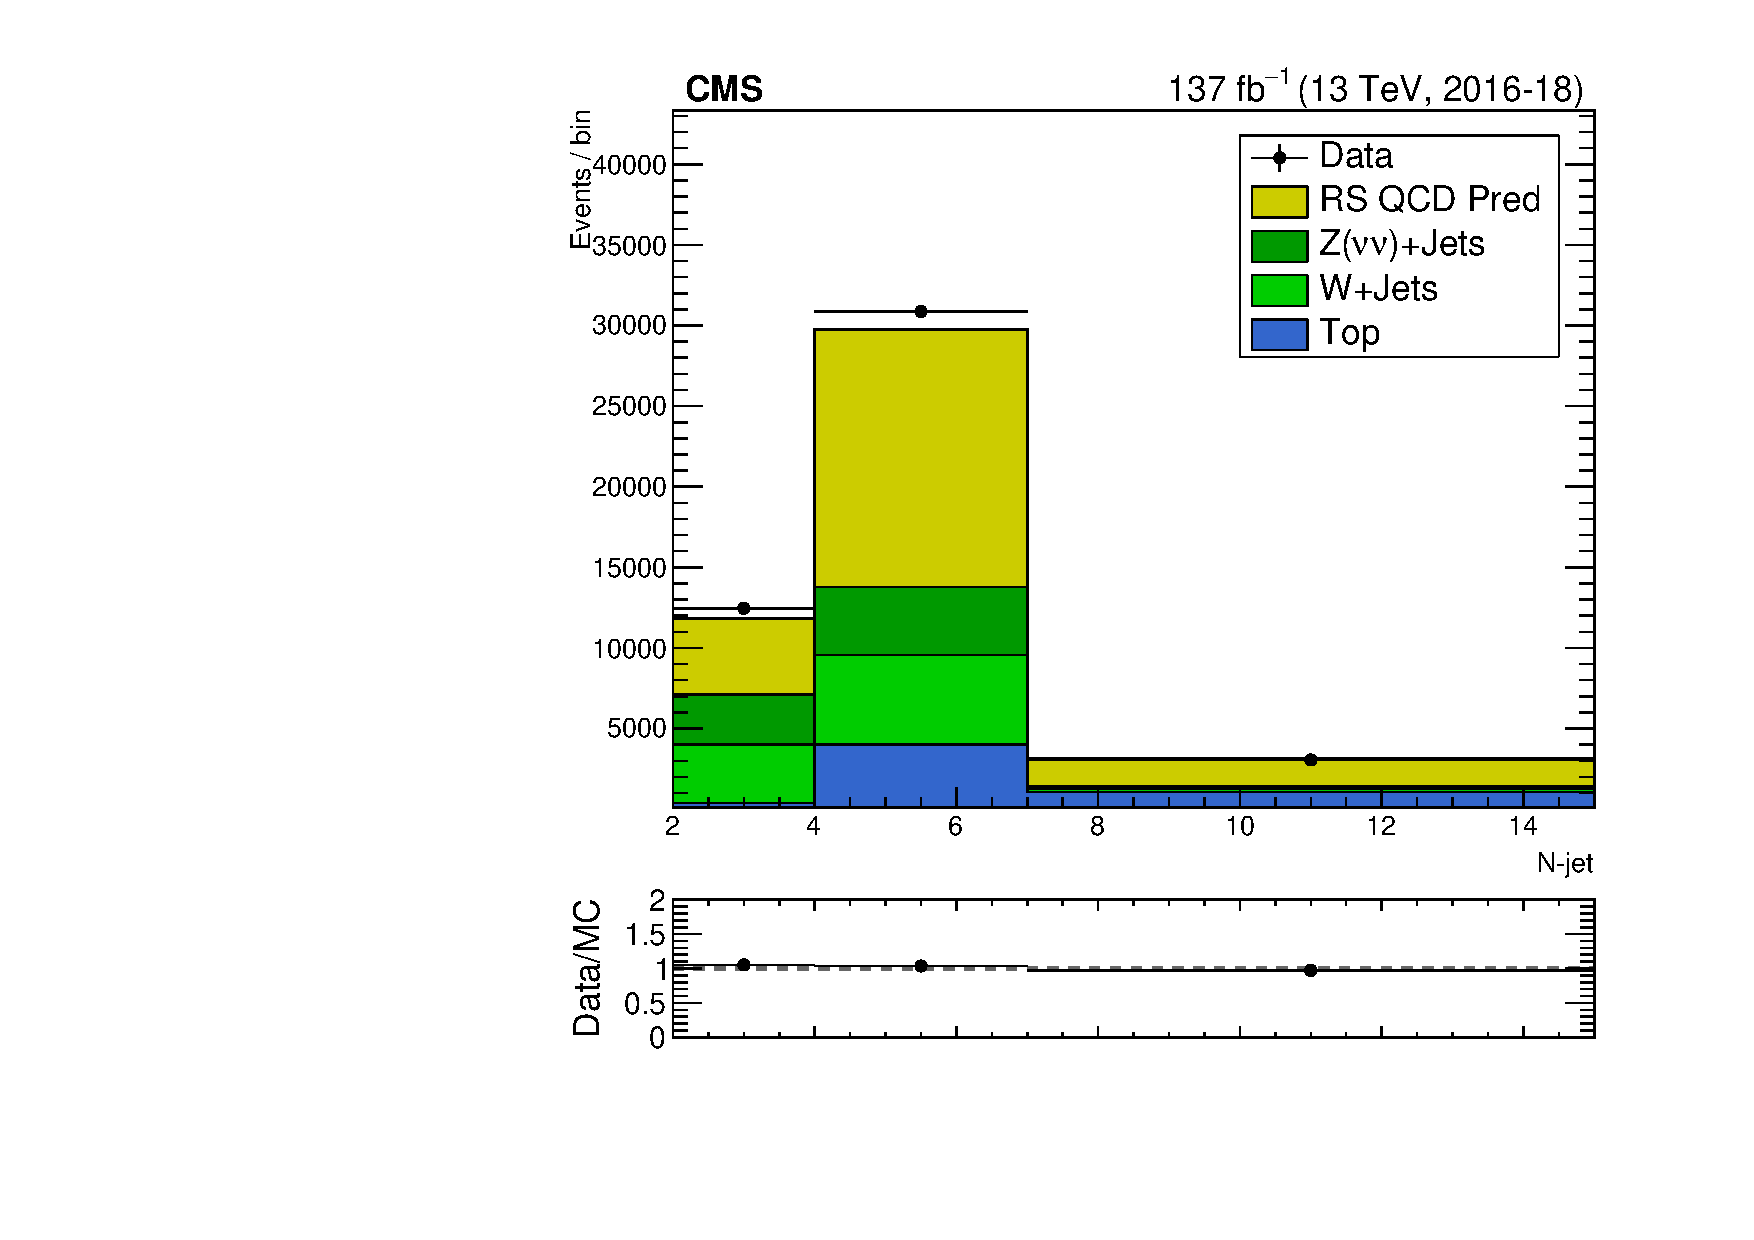
\includegraphics[width=0.46\textwidth]{figs/qcd/rs_data/c_crRSDPhiMT2InclusiveHT450to1200_h_nJet30.pdf}
    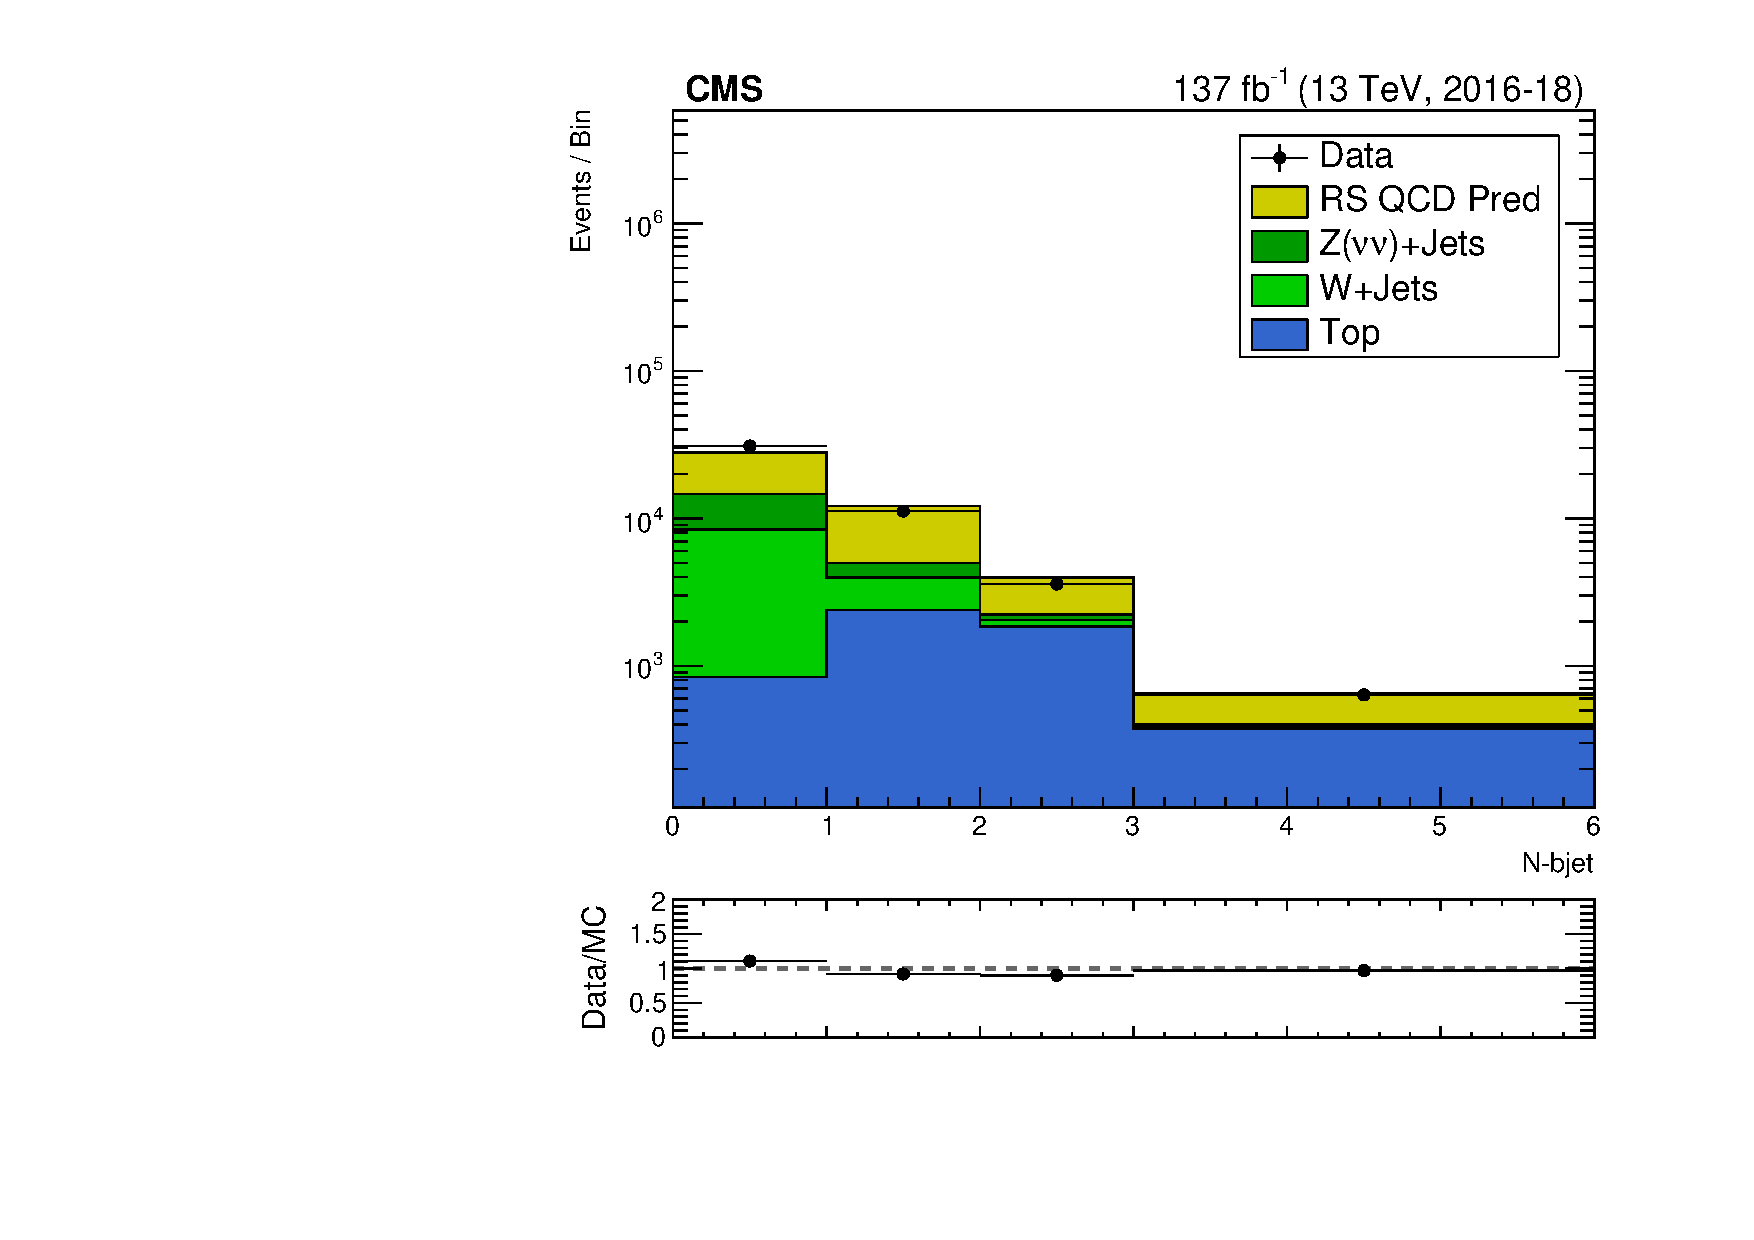
\includegraphics[width=0.46\textwidth]{figs/qcd/rs_data/c_crRSDPhiMT2InclusiveHT450to1200_h_nBJet20.pdf}
    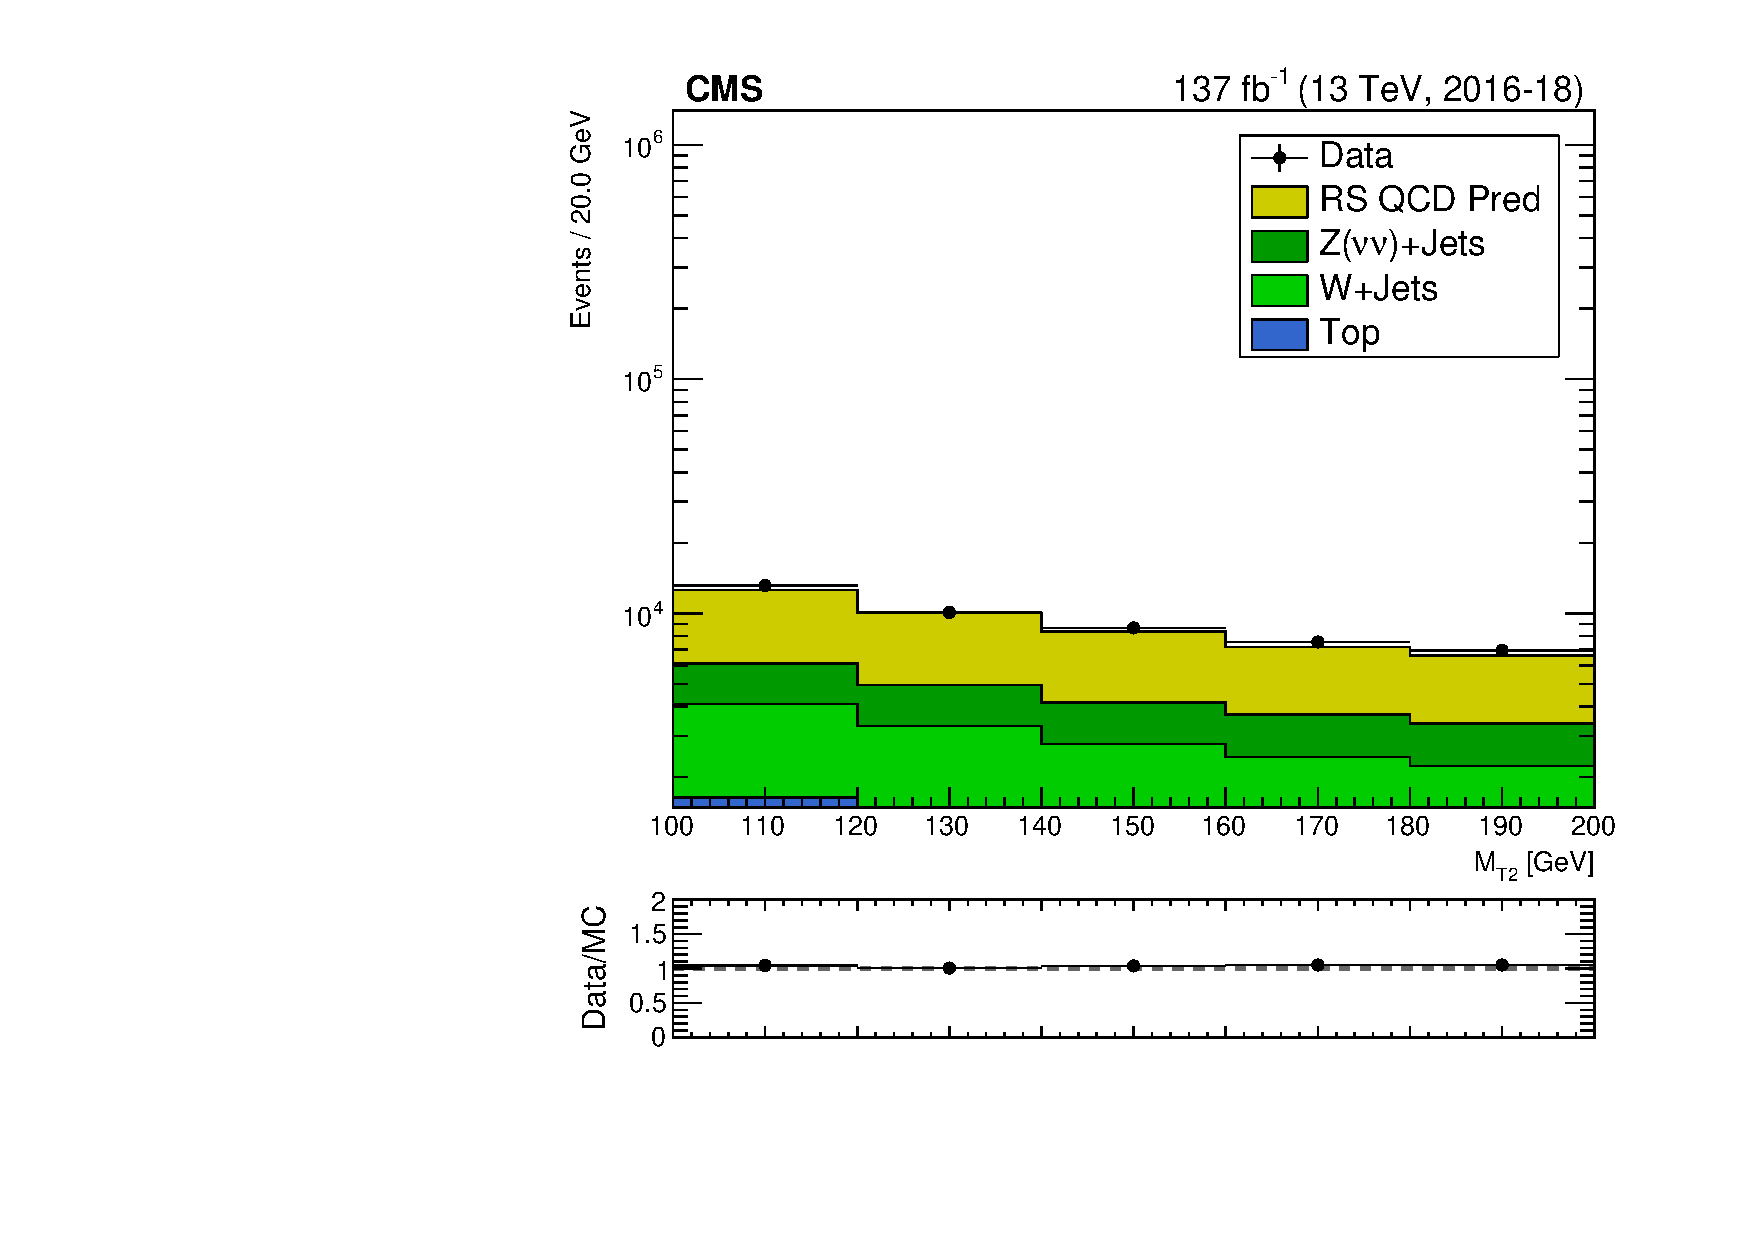
\includegraphics[width=0.46\textwidth]{figs/qcd/rs_data/c_crRSDPhiMT2InclusiveHT450to1200_h_mt2.pdf}
    \caption{Comparison of kinematic distributions for data and background in the $\mttwo$ sideband + inverted $\dpmin$ control region for $450<\Ht<$ 1200\GeV. The QCD background is from the
             rebalance and smear data-driven prediction. Non-QCD backgrounds are taken from Monte Carlo.
            }
    \label{Fig:rs_crRSDPhiMT2InclusiveHT450to1200}
  \end{center}
\end{figure}

\newpage
We can also look at total yields within each of the analysis topological regions in these 3 control regions. 
These are shown in Figures \ref{Fig:rs_dataCR_InvertDPhi}--\ref{Fig:rs_dataCR_DPhiMT2}.
In these plots, the electroweak background is data-driven using the same methods as in the main analysis.
Where the available statistics do not permit such a data-driven estimate, the electroweak contribution is taken directly from MC.
The gray bands represent the statistical error on the prediction combined with the systematics we assign, as discussed in Sec.~\ref{sec:rs_systematics}.
In all cases, data agrees with prediction within the assigned error.

\begin{figure}[htbp]
  \begin{center}
    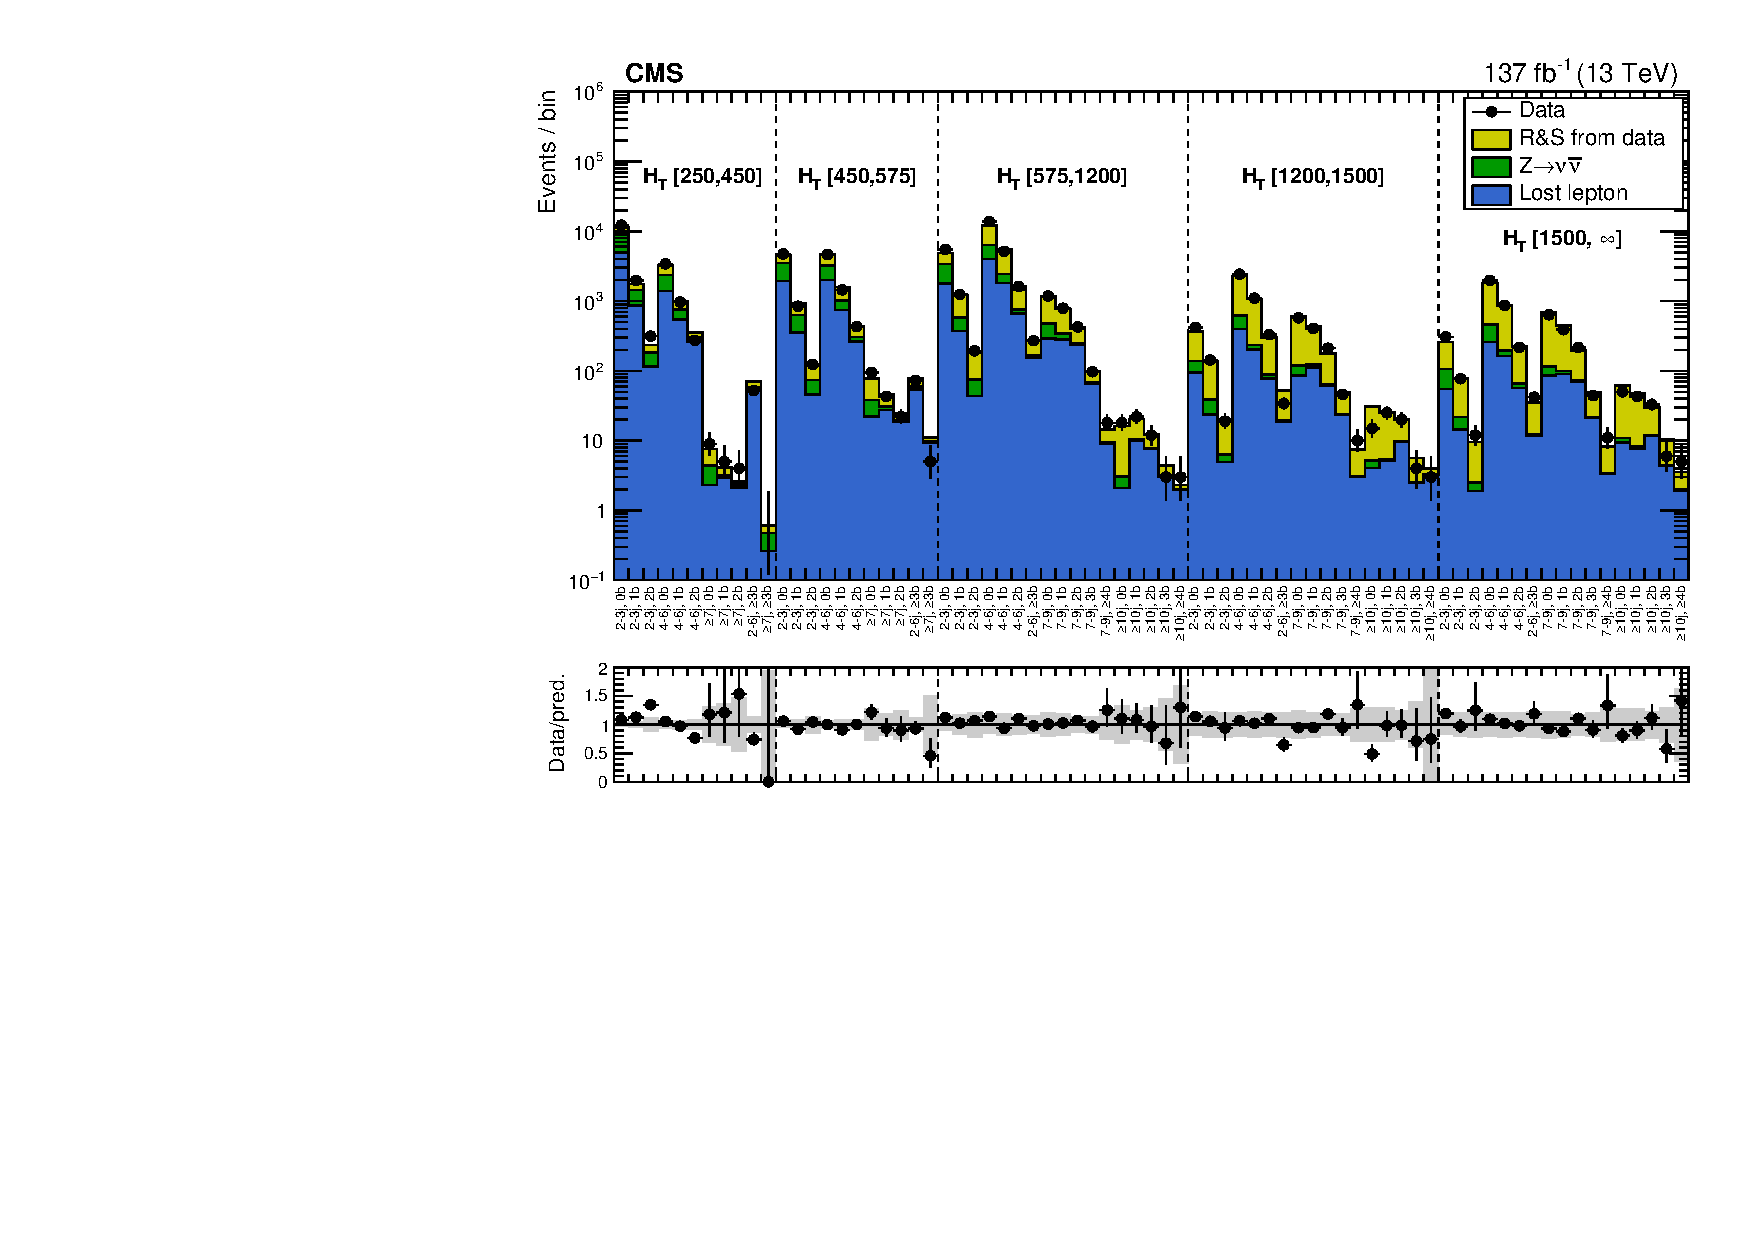
\includegraphics[width=0.99\textwidth]{figs/qcd/rs_data/comp_InvertDPhi.pdf}
    \caption{Data closure in the inverted-\dpmin control region. Electroweak backgrounds are data-driven, and the gray band in the ratio plot represents the statistical error on the prediction plus the systematic error we assign.}
    \label{Fig:rs_dataCR_InvertDPhi}
  \end{center}
\end{figure}

\begin{figure}[htbp]
  \begin{center}
    \includegraphics[width=0.99\textwidth]{figs/qcd/rs_data/comp_MT2SideBand.pdf}
    \caption{Data closure in the \mttwo Sideband control region. Electroweak backgrounds are data-driven, and the gray band in the ratio plot represents the statistical error on the prediction plus the systematic error we assign.}
    \label{Fig:rs_dataCR_MT2SideBand}
  \end{center}
\end{figure}

\begin{figure}[ht]
  \begin{center}
    \includegraphics[width=0.99\textwidth]{figs/qcd/rs_data/comp_DPhiMT2.pdf}
    \caption{Data closure in the inverted-\dpmin plus \mttwo Sideband control region. Electroweak backgrounds are data-driven, and the gray band in the ratio plot represents the statistical error on the prediction plus the systematic error we assign.}
    \label{Fig:rs_dataCR_DPhiMT2}
  \end{center}
\end{figure}

\section{Extension to monojet regions}

Rebalance and Smear is also used for estimating background from QCD events in the monojet signal regions.
The methodology is exactly the same as for the multijet case. The procedure is validated in an inverted-\dpmin dijet
control region, with exactly 2 jets, $\Ht>250$\GeV and $\ptmiss>250$\GeV. Fig.~\ref{Fig:rs_monojet_mc_validation} shows QCD MC
compared against the prediction from Rebalance and Smear applied to MC in this control region,
both inclusively and in the $30 < \pt(\mrm{jet 2}) < 60$\GeV
sideband nearest the monojet signal region. Good agreement is seen in both cases.

\begin{figure}[htp!]
  \begin{center}
    \includegraphics[width=0.49\textwidth]{figs/qcd/rs_data/monojet/mc_crRSInvertDPhibaseJ_htbins.pdf}
    \includegraphics[width=0.49\textwidth]{figs/qcd/rs_data/monojet/mc_crRSInvertDPhibaseJ_htbins_jet2pt_30_60.pdf}
    \caption{Closure between QCD MC and the prediction from Rebalance and Smear, in an inverted-\dpmin dijet
control region. The left plot is inclusive in jet \pt, while the right is in a $30 < \pt(\mrm{jet 2}) < 60$\GeV
sideband that is adjacent to the monojet signal region.
            }
    \label{Fig:rs_monojet_mc_validation}
  \end{center}
\end{figure}

\begin{figure}[htp!]
  \begin{center}
    \includegraphics[width=0.60\textwidth]{figs/qcd/rs_data/monojet/dataAll_crRSInvertDPhibaseJ_htbins.pdf}
    \caption{Closure between data and the prediction from Rebalance and Smear, in an inverted-\dpmin dijet
control region. Electroweak backgrounds are from MC.
            }
    \label{Fig:rs_monojet_data_validation}
  \end{center}
\end{figure}

Fig.~\ref{Fig:rs_monojet_data_validation} shows closure between data and the Rebalance and Smear method applied to data
in the same dijet control region. Electroweak backgrounds are from MC. Again, good agreement is seen.

%\newpage
\section{Systematic uncertainties}
\label{sec:rs_systematics}

Sections \ref{sec:rs_jrt_core} through \ref{sec:rs_sigmasoft} study the effects of varying
parameters in the jet response templates or the rebalancing procedure on the final estimate.
In Sec. \ref{sec:rs_finalsyst}, we use these to assess systematic uncertainties on the final estimate.

\subsection{Effect of modifying width of jet response core}
\label{sec:rs_jrt_core}

Here we study in both MC and data how the rebalance and smear prediction is affected by increasing the width of the Gaussian core component of the jet response templates. 
The core of the response is identified by fitting a Gaussian to a narrow window around the peak response, as described in Sec.~\ref{sec:jrt_fits}.

In MC, we test the effect by increasing the width of the Gaussian core by a uniform factor for all jet response templates. 
The procedure for performing this widening is again described in Sec.~\ref{sec:jrt_fits}. 
Figure~\ref{Fig:rs_modify_core} shows the effect of increasing the width of the Gaussian core by 10\% and 25\% on the rebalance and smear predictions from MC in the 
analysis topological regions.

\begin{figure}[ht]
  \begin{center}
    \includegraphics[width=1.0\textwidth]{figs/qcd/rs_mc/mc_coreWidth.pdf}
    \caption{Comparison of yields in topological regions for QCD from MC (yellow points), standard \rs prediction from MC (black points), \rs with response core width + 10\% (blue points), and
             \rs with response core width + 25\% (red points). The bottom histogram shows the ratios of yields in topological regions for response core width + 10\% and response core width + 25\%
             with respect to the standard \rs prediction.
            }
    \label{Fig:rs_modify_core}
  \end{center}
\end{figure}

We also study this in data by varying the width of the core by the jet energy resolution (JER) smear factor uncertainties derived by the JetMET group, listed in Table \ref{tab:jrt_jersfs}.
The result of varying the width up/down by this amount is shown in Figure~\ref{Fig:rs_data_JER_var}. Variations in each \Ht-region are shown in colored text near
the top of the plot. These are used to derive a systematic in Sec. \ref{sec:rs_finalsyst}.

\begin{figure}[ht]
  \begin{center}
    \includegraphics[width=1.0\textwidth]{figs/qcd/rs_data/data_JER_systVar.pdf}
    \caption{Comparison of yields in topological regions for \rs from data for nominal JER (black), JER varied UP (green), and JER varied DOWN (red). Variations with respect to the nominal yield
      in each \Ht-region are shown in colored text.
            }
    \label{Fig:rs_data_JER_var}
  \end{center}
\end{figure}


\subsection{Effect of modifying size of jet response tail}
\label{sec:rs_jrt_tail}

Next, we study in Monte Carlo how the \rs method is affected by increasing the size of the non-Gaussian tail component of the jet response templates.
As described in Sec.~\ref{sec:jrt_fits}, the tail is defined as simply the subtraction of the fitted Gaussian core from the raw template.
For this study, we increase the size of the tails by 25\% and 50\% for all templates, simply by scaling the tail components by a constant factor
(while also scaling down the core normalization by an appropriate amount to preserve normalization).
Figure~\ref{Fig:rs_modify_tail} shows the result of this scaling in each of the analysis topological regions, and Table~\ref{tab:rs_table_modify_tail}
summarizes the change in yields for each \Ht region.

\begin{figure}[h]
  \begin{center}
    \includegraphics[width=1.0\textwidth]{figs/qcd/rs_mc/mc_tailSize.pdf}
    \caption{Comparison of yields in topological regions for QCD from MC (yellow points), standard \rs prediction from MC (black points), \rs with response tail size + 25\% (red points), and
             \rs with response tail size + 50\% (blue points). The bottom histogram shows the ratios of yields in topological regions for response tail size + 25\% and response tail size + 50\%
             with respect to the standard \rs prediction.
            }
    \label{Fig:rs_modify_tail}
  \end{center}
\end{figure}

\begin{table}[h!]
\caption{Effect of increasing the size of the jet response tails in each $\Ht$ region.
\label{tab:rs_table_modify_tail}}
\centering
\begin{tabular}{l|cc}
\hline
 & tail+25\% / standard \rs & tail+50\% / standard \rs \\
\hline
very low $\Ht$ & 1.17 & 1.34 \\
low $\Ht$ & 1.18 & 1.33 \\
medium $\Ht$ & 1.24 & 1.47 \\
high $\Ht$ & 1.25 & 1.50 \\
extreme $\Ht$ & 1.25 & 1.49 \\
\hline
\end{tabular}
\end{table}


\subsection{Effect of shifting mean of jet response}
\label{sec:rs_jrt_mean}

Next, we study in Monte Carlo how the \rs method is affected by shifting the mean of each jet response template by a constant amount,
chose here to by +4\%. This simulates deriving the jet response templates on a sample that has a jet energy scale that is 4\% higher 
than the sample on which the templates are used for a prediction.
Figure~\ref{Fig:rs_modify_mean} shows the effect of shifting the jet response mean by +4\% on the \rs predictions from MC in the analysis topological regions.
Table~\ref{tab:rs_table_modify_mean} summarizes the change in yields for each $\Ht$ region.

\begin{figure}[ht]
  \begin{center}
    \includegraphics[width=1.0\textwidth]{figs/qcd/rs_mc/mc_meanShift.pdf}
    \caption{Comparison of yields in topological regions for QCD from MC (yellow points), standard \rs prediction from MC (black points), and \rs with response mean shifted higher by 4\% (blue points).
             The bottom histogram shows the ratio of yields in topological regions for response mean shifted higher by 4\% with respect to the standard \rs prediction.
            }
    \label{Fig:rs_modify_mean}
  \end{center}
\end{figure}

\begin{table}[h]
\caption{Effect of shifting the mean of the jet response in each $\Ht$ region.
\label{tab:rs_table_modify_mean}}
\centering
\begin{tabular}{l|c}
\hline
 & mean+4\% / standard \rs \\
\hline
very low $\Ht$ & 0.82 \\
low $\Ht$ & 0.69 \\
medium $\Ht$ & 0.75 \\
high $\Ht$ & 0.99 \\
extreme $\Ht$ & 1.11 \\
\hline
\end{tabular}
\end{table}


\subsection{Effect of modifying $\sigma_\mrm{T}^\mrm{soft}$}
\label{sec:rs_sigmasoft}

Finally, we check how the \rs prediction changes based on the value chosen for the $\sigma_\mrm{T}^\mrm{soft}$ parameter used in rebalancing.
The parameter controls how tightly the \vMet is constrained to be near 0 post-rebalancing.
It is nominally chosen to be 20\GeV based on the width of the \ptmiss distribution in minimum-bias data. 
Figure~\ref{Fig:rs_modify_sigmasoft} shows the effect of changing $\sigma_\mrm{T}^\mrm{soft}$ by $\pm20$\% (i.e. to 15 or 25\GeV)
on the \rs prediction from MC in the analysis topological regions.
Table~\ref{tab:rs_table_modify_sigmasoft} summarizes the change in yields for each $\Ht$ region.

\begin{figure}[ht]
  \begin{center}
    \includegraphics[width=1.0\textwidth]{figs/qcd/rs_mc/mc_sigmasoft.pdf}
    \caption{Comparison of yields in topological regions for QCD from MC (yellow points), standard \rs prediction from MC (black points), \rs with $\sigma_\mrm{T}^\mrm{soft}$ = 15\GeV (blue points), and
             \rs with $\sigma_\mrm{T}^\mrm{soft}$ = 25\GeV (red points). The bottom histogram shows the ratios of yields in topological regions for $\sigma_\mrm{T}^\mrm{soft}$ = 15\GeV and
             $\sigma_\mrm{T}^\mrm{soft}$ = 25\GeV with respect to the standard \rs prediction.
            }
    \label{Fig:rs_modify_sigmasoft}
  \end{center}
\end{figure}

\begin{table}[ht]
\caption{Effect of changing $\sigma_\mrm{T}^\mrm{soft}$ in each $\Ht$ region.
\label{tab:rs_table_modify_sigmasoft}}
\centering
\begin{tabular}{l|cc}
\hline
 & $\sigma_\mrm{T}^\mrm{soft}$ = 15\GeV / standard \rs & $\sigma_\mrm{T}^\mrm{soft}$ = 25\GeV / standard \rs \\
\hline
very low $\Ht$ & 0.99 & 1.00 \\
low $\Ht$ & 1.08 & 0.97 \\
medium $\Ht$ & 1.12 & 1.05 \\
high $\Ht$ & 1.07 &1.06 \\
extreme $\Ht$ & 1.05 & 1.04 \\
\hline
\end{tabular}
\end{table}


\subsection{Final systematic uncertainties assessed on estimate}
\label{sec:rs_finalsyst}
We assign systematic uncertainties from three main sources: jet energy resolution uncertainty, template tail size uncertainty, and $\sigma_{T}^{soft}$ uncertainty.
As seen from Figures~\ref{Fig:rs_data_JER_var}, \ref{Fig:rs_modify_tail}, \ref{Fig:rs_modify_sigmasoft}, the effect of varying these features has no strong
\Nj/\Nb dependence and varies mainly by \Ht region. Therefore, we assign these systematics by \Ht region and take them as correlated across all bins. Due to low statistics,
we combine the Very Low and Low \Ht regions when deriving systematics.
For JER uncertainty, we take the maximum yield variation after varying JER up/down in data. For tail size uncertainty, we take the MC yield variation resulting from a 25\% increase
in tail size. And for $\sigma_\mrm{T}^\mrm{soft}$ variation, we take the maximum yield variation after varying $\sigma_\mrm{T}^\mrm{soft}$ by $\pm5$\GeV (20\%). The results are given in
Table~\ref{tab:rs_table_systematics}.

\begin{table}[h]
\caption{Systematics assigned to each \Ht-region based on uncertainties in JER, tail size modeling, and $\sigma_\mrm{T}^\mrm{soft}$.
The ``Total'' column is the 3 systematics added in quadrature.
\label{tab:rs_table_systematics}}
\centering
\begin{tabular}{r|ccc|c}
\hline
 & JER & Tail size & $\sigma_{T}^{soft}$ & Total \\
\hline
Very Low \Ht & 5\% & 17\% & 1\% & 18\% \\
Low \Ht & 14\% & 17\% & 1\% & 22\% \\
Medium \Ht & 18\% & 24\% & 12\% & 32\% \\
High \Ht & 13\% & 25\% & 7\% & 29\% \\
Extreme \Ht & 10\% & 25\% & 5\% & 27\% \\
Monojet, 0b & 10\% & 21\% & 17\% & 29\% \\
Monojet, $\geq1$b & 5\% & 8\% & 25\% & 27\% \\
\hline
\end{tabular}
\end{table}

As the above systematics are integrated across all variables except \Ht, we assign final systematics on the modeling of \Nj and \Nb shapes,
derived from the \Nj and \Nb plots in the inverted-\dpmin control region (Figure \ref{Fig:rs_crRSInvertDPhiInclusiveHT1200toInf}). These systematics
grow with \Nj and \Nb and are correlated within each \Ht region. Table~\ref{tab:rs_njnb_systematics} lists the assigned systematics.

\begin{table}[h]
\caption{Assigned systematics to each \Nj/\Nb bin, based on observed discrepancies in \Nj/\Nb shapes in the inverted-\dpmin control regions.
The uncertainties are taken as completely correlated within each \Ht region, and uncorrelated between \Ht regions.
The signs indicate the direction of correlation.
\label{tab:rs_njnb_systematics}}
\centering
\begin{tabular}{c|cc}
\hline
 & $\Ht<1200$ & $\Ht\geq1200$ \\
\hline
2-3 jets      & $0$\%   & $2$\% \\
4-6 jets      & $1$\%  & $3$\% \\
2-6 jets      & $1$\%   & $3$\% \\
7-9 jets      & $-8$\%  & $-7$\% \\
$\geq7$ jets  & $-8$\%  & $-7$\% \\
$\geq10$ jets & $-20$\% & $-19$\% \\
\hline
0 b-jets       & $5$\%     & $4$\% \\
1 b-jets       & $-9$\%    & $-5$\% \\
2 b-jets       & $-9$\%   & $-5$\% \\
3 b-jets       & $-14$\%   & $-16$\% \\
$\geq3$ b-jets & $-14$\%   & $-16$\% \\
$\geq4$ b-jets & $-14$\%   & $-16$\% \\
\end{tabular}
\end{table}
